% main.tex
% Memoria P.D.S. (Release Notes) - ISO/IEC/IEEE 26515:2024 e ISO 15289
% Producto documentado: EthosHub (ethoshubB / ethoshubF)
% Estructura alineada al índice indice_documentacion_iso26515.md (Sprints 0 a 5)

\documentclass[10pt, a4paper, twoside]{report} % Base a 10pt para notas de versión

% 01_packages.tex
% Paquetes esenciales para la Memoria P.D.S. (ISO 26515 Ágil)

\usepackage[utf8]{inputenc}
\usepackage[T1]{fontenc}
\usepackage[spanish,es-tabla]{babel}

% Familias Tipográficas
\usepackage{mathptmx}  % Cuerpo: Serif (Times New Roman) - Compacto
\usepackage{helvet}    % Títulos: Sans-serif (Helvetica)
\usepackage{courier}   % User Stories / Tags: Monospace (Courier New)

% Geometría y Layout Minimalista
\usepackage{geometry}  
\usepackage{setspace}  
\usepackage{fancyhdr}  
\usepackage{lastpage}  
\usepackage{titlesec}  

% Gráficos, Colores y Tablas
\usepackage{graphicx}      
\usepackage[table]{xcolor} 
\usepackage{fontawesome5}  
\usepackage{amssymb}       
\usepackage{tabularx}      
\usepackage{booktabs}      

% Cajas de Diseño y Listas
\usepackage[most]{tcolorbox}
\usepackage{enumitem}

% Bloques de código fuente (Documentation as Code)
\usepackage{listings}

% Diagramas vectoriales (C4, ER, secuencia)
\usepackage{tikz}
\usetikzlibrary{shapes.geometric, arrows.meta, positioning, fit, backgrounds, calc}

% Navegación PDF
\usepackage{hyperref}
% 03_fonts_colors.tex
% Configuración de Tipografía y Paleta de Colores de Pruebas

\renewcommand{\rmdefault}{ptm} 
\renewcommand{\sfdefault}{phv} 
\renewcommand{\ttdefault}{pcr} 

% Paleta Corporativa
\definecolor{colorPrimario}{HTML}{1A75FB}   % Azul Corporativo
\definecolor{colorSecundario}{HTML}{4CAF50} % Verde
\definecolor{colorAcento}{HTML}{FFC107}     % Amarillo

% Colores de Estado de Pruebas (Pass/Fail)
\definecolor{bgPass}{HTML}{4CAF50}          % Verde Éxito
\definecolor{bgFail}{HTML}{F44336}          % Rojo Fallo
\definecolor{bgBlocked}{HTML}{9E9E9E}       % Gris Bloqueado

% Colores para Tablas de Datos
\definecolor{headerTabla}{HTML}{BBDDFC}     % Fondo cabeceras
\definecolor{grisTecnico}{HTML}{F5F5F5}     % Celdas alternadas y fondos
\definecolor{grisISO}{HTML}{5D6363}

\definecolor{bgNota}{HTML}{BBDDFC}          % Fondo Notas
\definecolor{bordeNotaTecnica}{HTML}{2196F3}% Borde azul para Notas Técnicas
\definecolor{textVerde}{HTML}{2E7D32}       % Texto Verde para User Stories
\definecolor{bgAdvertencia}{HTML}{FFF3E0}   % Fondo advertencia
% 02_layout.tex
% Geometría, Encabezados y Trazabilidad (IEEE 1012-2024)

% 1. Configuración de Márgenes Exactos
\geometry{
    a4paper,
    inner=2.5cm,       
    outer=2.5cm,       
    top=2.5cm,       
    bottom=2.5cm,    
    includehead,     
    includefoot,     
    headheight=28pt, 
    headsep=0.4cm,   
    footskip=1.0cm   
}
\singlespacing

% Microtipografía: permite a TeX encontrar mejores cortes de línea (reduce
% los avisos Overfull/Underfull en texto justificado sin alterar el contenido).
\emergencystretch=3em

% Portada de capítulo estilo "libro" (alineada al Manual Técnico): el título del
% capítulo ocupa su propia plana con un rótulo "CAPÍTULO N" en gran tamaño y un
% breve resumen declarado con \resumenCapitulo{...}. El contenido inicia en la
% página siguiente.
\titleformat{\chapter}[display]
  {\sffamily\bfseries\color{colorPrimario}}
  {\filright\fontsize{13}{15}\selectfont\color{grisISO}\MakeUppercase{Capítulo \thechapter}}
  {0.35cm}
  {\fontsize{25}{29}\selectfont\filright}
  []
\titlespacing*{\chapter}{0pt}{55pt}{24pt}

% \resumenCapitulo{texto}: sinopsis breve bajo el título del capítulo, en la misma
% plana. Cierra con \clearpage para que el contenido empiece en la página siguiente.
\newcommand{\resumenCapitulo}[1]{%
  \vspace{0.5cm}%
  {\color{colorAcento}\rule{2.5cm}{2pt}}\par
  \vspace{0.45cm}%
  {\normalfont\sffamily\fontsize{11}{15}\selectfont\color{grisISO!95!black}%
   \itshape #1\par}%
  \clearpage}

\titleformat{\section}[hang]
  {\sffamily\bfseries\fontsize{14}{16.8}\selectfont\color{colorPrimario}}
  {\thesection.}
  {1em}{}

% ==========================================
% VARIABLES DINÁMICAS DE SPRINT
% ==========================================
\newcommand{\currentSprint}{Sprint \# - Estado}
\newcommand{\currentTag}{release/v0.0.0}
\newcommand{\currentTaskID}{Gestor Tareas: ID}
\newcommand{\docOwner}{Propietario: Nombre}

\newcommand{\setSprint}[1]{\renewcommand{\currentSprint}{#1}}
\newcommand{\setTag}[1]{\renewcommand{\currentTag}{#1}}
\newcommand{\setTaskID}[1]{\renewcommand{\currentTaskID}{#1}}
\newcommand{\setDocOwner}[1]{\renewcommand{\docOwner}{#1}}

% ==========================================
% ENCABEZADOS Y PIES (Documentation as Code)
% ==========================================
\pagestyle{fancy}
\fancyhf{} 

% Encabezado: Logo (Izq) | Estado Sprint (Centro) | Branch/Tag (Der)
\fancyhead[L]{
\includegraphics[height=0.5cm, keepaspectratio]{assets/img/bytebusters/logo_horizontal.png}}
\fancyhead[C]{\sffamily\footnotesize\textcolor{colorPrimario}{\currentSprint}}
\fancyhead[R]{\fontfamily{pcr}\footnotesize\textcolor{grisISO}{\currentTag}}

% Pie de Página: Trazabilidad (Izq) | Owner y Paginación (Der)
\fancyfoot[L]{\sffamily\footnotesize\textcolor{grisISO}{\currentTaskID}}
\fancyfoot[R]{\sffamily\footnotesize\textcolor{grisISO}{Byte Busters S.R.L.\ | Pág. \thepage\ de \pageref{LastPage}}}

\renewcommand{\headrulewidth}{0.4pt}
\renewcommand{\footrulewidth}{0.4pt}
\renewcommand{\headrule}{\hbox to\headwidth{\color{grisISO}\leaders\hrule height \headrulewidth\hfill}}
\renewcommand{\footrule}{\hbox to\headwidth{\color{grisISO}\leaders\hrule height \footrulewidth\hfill}}

\hypersetup{colorlinks=true, linkcolor=colorPrimario, urlcolor=colorPrimario}

\hypersetup{
    colorlinks=true, 
    linkcolor=colorPrimario, 
    urlcolor=colorPrimario, 
    pdftitle={Documentación por Sprint ISO/IEC/IEEE 26515:2024},
    pdfauthor={Byte Busters S.R.L.}
    }
% 04_macros.tex
% Componentes de Control de Calidad (Bug Reports y Test Cases)

% 1. Macros de Estado (Celdas condicionales)
\newcommand{\estadoPass}{\cellcolor{bgPass}\textcolor{white}{\sffamily\bfseries PASS}}
\newcommand{\estadoFail}{\cellcolor{bgFail}\textcolor{white}{\sffamily\bfseries FAIL}}
\newcommand{\estadoBlocked}{\cellcolor{bgBlocked}\textcolor{white}{\sffamily\bfseries BLOCKED}}
\newcommand{\comando}[1]{{\fontfamily{pcr}\fontsize{9}{10.8}\selectfont\colorbox{grisTecnico}{\texttt{#1}}}}

% 2. Entorno: Especificación de Casos de Prueba (Ejecución)
% Usa tipografía sans-serif a 9pt para alta densidad de datos
\newenvironment{TablaCasoPrueba}{
    \renewcommand{\arraystretch}{1.5}
    \vspace{0.3cm}
    \noindent
    \fontsize{9}{10.8}\selectfont\sffamily
    \tabularx{\textwidth}{|c|X|X|c|}
    \hline
    \rowcolor{headerTabla}
    \textbf{Paso \#} & \textbf{Acción (Instrucción)} & \textbf{Resultado Esperado (Criterio)} & \textbf{Estado} \\
    \hline
}{
    \endtabularx
    \vspace{0.3cm}
}

% 3. Entorno: Reporte de Defectos (Bug Report)
\newenvironment{BugReport}{
    \renewcommand{\arraystretch}{1.5}
    \vspace{0.3cm}
    \noindent
    \fontsize{9}{10.8}\selectfont\sffamily
    \tabularx{\textwidth}{|>{\bfseries\color{colorPrimario}}l|X|}
    \hline
    \rowcolor{headerTabla}
    Campo & Contenido \\
    \hline
}{
    \endtabularx
    \vspace{0.3cm}
}

% Nota Técnica general preservada
\newtcolorbox{NotaTecnica}{
    colback=white,
    colframe=bordeNotaTecnica,
    boxrule=1.2pt,
    arc=2pt,
    title={\faInfoCircle\ \textbf{Nota de Configuración}},
    coltitle=bordeNotaTecnica,
    fonttitle=\sffamily,
    attach title to upper=\par\vspace{0.2em}
}

% 2. Aviso de Cambio Crítico (Breaking Changes)
\newtcolorbox{BreakingChange}{
    colback=bgAdvertencia,
    colframe=colorAcento,
    boxrule=1.5pt,
    leftrule=6pt,
    arc=2pt,
    title={\faExclamationTriangle\ \textbf{Cambio Crítico (Breaking Change)}},
    coltitle=black,
    fonttitle=\sffamily,
    attach title to upper=\par\vspace{0.2em}
}

% 3. Checklist de Definition of Done (DoD)
\newlist{ChecklistDoD}{itemize}{1}
\setlist[ChecklistDoD]{label=$\square$, leftmargin=*}

% 4. Tabla de Historias vs. Documentación
\newenvironment{TablaHSDoc}{
    \renewcommand{\arraystretch}{1.5}
    \vspace{0.3cm}
    \noindent
    \fontsize{10}{12}\selectfont\sffamily
    \tabularx{\textwidth}{|l|X|X|X|}
    \hline
    \rowcolor{headerTabla}
    \textbf{ID Historia} & \textbf{Funcionalidad} & \textbf{Manual Usuario Act.?} & \textbf{Manual Técnico Act.?} \\
    \hline
}{
    \endtabularx
    \vspace{0.3cm}
}

% Cajas originales de advertencia preservadas
\newtcolorbox{AlertaDefecto}{colback=white, colframe=bgFail, boxrule=1.2pt, arc=2pt, title={\faBug\ \textbf{Defecto Crítico Detectado}}, coltitle=bgFail, fonttitle=\sffamily, attach title to upper=\par\vspace{0.2em}}

\begin{document}

% ============================= FRONT MATTER =============================
\begin{titlepage}
    \thispagestyle{empty}
    \sffamily

    % =====================================================================
    % SECCIÓN SUPERIOR — IDENTIFICACIÓN INSTITUCIONAL
    % =====================================================================
    \vspace*{-3.0cm}
    \begin{center}
        
\includegraphics[width=0.36\textwidth]{assets/img/umss/logoUMSS.png}\par
        \vspace{0.3cm}
        {\large\textbf{Universidad Mayor de San Simón}\par}
        {\normalsize\textbf{Facultad de Ciencias y Tecnología}\par}
        {\normalsize Licenciatura en Ingeniería de Sistemas\par}
    \end{center}

    % Barra de clasificación documental (banda superior)
    \vspace{0.5cm}
    \begin{center}
        \colorbox{colorPrimario}{%
            \parbox{0.96\textwidth}{\centering
                \color{white}\footnotesize\bfseries
                DOCUMENTO CONTROLADO \quad$\bullet$\quad
                CLASIFICACIÓN: CONFIDENCIAL \quad$\bullet$\quad
                CONVOCATORIA CPTIS-2302-2026%
            }%
        }
    \end{center}

    % =====================================================================
    % SECCIÓN CENTRAL — TÍTULO DEL ARTEFACTO
    % =====================================================================
    \vspace{0.8cm}
    \begin{center}
        \rule{\textwidth}{1.2pt}\par
        \vspace{0.35cm}
        {\Huge\bfseries\color{colorPrimario} Memoria de Producto\par}
        \vspace{0.15cm}
        {\LARGE\bfseries de Software\par}
        \vspace{0.35cm}
        {\large Plataforma \textbf{EthosHub}\par}
        {\normalsize\itshape Release Notes por Sprint --- Sistema Generador de Portafolios Digitales\par}
        \vspace{0.3cm}
        \rule{\textwidth}{1.2pt}\par
    \end{center}

    % =====================================================================
    % BLOQUE DE IDENTIFICACIÓN DOCUMENTAL (ISO/IEC/IEEE 26515:2024)
    % =====================================================================
    \vspace{0.7cm}
    \begin{center}
        \renewcommand{\arraystretch}{1.2}
        \fontsize{9}{10.8}\selectfont
        \begin{tabularx}{0.92\textwidth}{|>{\bfseries\color{colorPrimario}}l|X|}
            \hline
            \rowcolor{headerTabla}
            \multicolumn{2}{|l|}{\sffamily\textbf{Identificación del documento (ISO/IEC/IEEE 15289:2024)}} \\
            \hline
            Identificador (Doc ID) & \texttt{MEM-PDS-ETHOSHUB-2.0.0} \\
            \hline
            \rowcolor{grisTecnico}
            Versión & 2.0.0 \\
            \hline
            Estado & Aprobado \\
            \hline
            \rowcolor{grisTecnico}
            Fecha de emisión & 15 de junio de 2026 \\
            \hline
            Norma de referencia & ISO/IEC/IEEE 26515:2024 \,$\cdot$\, ISO/IEC/IEEE 15289:2024 \\
            \hline
            \rowcolor{grisTecnico}
            Tipo de artefacto & Memoria de Producto de Software (Release Notes) \\
            \hline
            \rowcolor{headerTabla}
            \multicolumn{2}{|l|}{\sffamily\textbf{Proponente y supervisión}} \\
            \hline
            Razón social del proponente & Byte Busters S.R.L. \\
            \hline
            \rowcolor{grisTecnico}
            Representante legal & Juan Diego Pardo Pozo \\
            \hline
            Correo de contacto & contacto.bytebusters@gmail.com \\
            \hline
            \rowcolor{grisTecnico}
            Teléfono & +591 60349460 \\
            \hline
            Consultor TIS supervisor & Corina Justina Flores Villarroel \\
            \hline
        \end{tabularx}
    \end{center}

    \vfill
    \begin{center}
        {\normalsize Cochabamba, Bolivia \,$\cdot$\, Junio de 2026\par}
    \end{center}
\end{titlepage}


\begingroup
  \makeatletter \let\ps@plain\ps@empty \makeatother
  \pagestyle{empty}
  % =============================================================================
% HISTORIAL DE REVISIONES Y TRAZABILIDAD (ISO/IEC/IEEE 15289:2024)
% =============================================================================
\chapter*{Historial de Revisiones y Trazabilidad}
\addcontentsline{toc}{chapter}{Historial de Revisiones y Trazabilidad}
\markboth{Historial de Revisiones y Trazabilidad}{}

La presente \textbf{Memoria de Producto de Software (P.D.S.)} consolida las
\textit{Release Notes} incrementales de la plataforma \textbf{EthosHub}, documentadas
Sprint a Sprint conforme al estándar \textbf{ISO/IEC/IEEE 26515:2024} (desarrollo de
información para usuarios en entornos ágiles) y a \textbf{ISO/IEC/IEEE 15289:2024}
(productos de información del ciclo de vida del software). Cada versión emitida queda
trazada en los registros siguientes, garantizando la responsabilidad
(\textit{accountability}) sobre el incremento de software descrito.\par

\section*{Control de Versiones del Documento}
\noindent
\renewcommand{\arraystretch}{1.4}
\fontsize{9}{10.8}\selectfont\sffamily
\begin{tabularx}{\dimexpr\textwidth-2pt\relax}{|c|c|X|c|}
\hline
\rowcolor{headerTabla}
\textbf{Versión} & \textbf{Fecha} & \textbf{Incremento documentado} & \textbf{Estado} \\
\hline
0.1.0 & 2026-03-28 & Sprint 0: incepción, arquitectura C4, ER preliminar y boilerplate FE/BE. & Aprobado \\
\hline
\rowcolor{grisTecnico}
1.0.0 & 2026-04-11 & Sprint 1: seguridad, autenticación, JWT y layouts base del frontend. & Aprobado \\
\hline
1.1.0 & 2026-04-25 & Sprint 2: habilidades/skills, dominio transaccional, CRUD y pruebas unitarias. & Aprobado \\
\hline
\rowcolor{grisTecnico}
1.2.0 & 2026-05-09 & Sprint 3: vitrina de proyectos, conexiones externas, tiempo real, CV Studio y Talent Discovery. & Aprobado \\
\hline
1.3.0 & 2026-05-23 & Sprint 4: visibilidad/privacidad, QA, refuerzo OWASP, pruebas E2E y accesibilidad. & Aprobado \\
\hline
\rowcolor{grisTecnico}
2.0.0 & 2026-06-06 & Sprint 5: estadísticas, despliegue monolítico, backups, Release Notes y cierre de versión. & Aprobado \\
\hline
\end{tabularx}\normalfont\normalsize
\par\vspace{0.5cm}

\section*{Roles del Equipo de Producto}
La elaboración y validación de esta memoria fue responsabilidad del equipo de
\textbf{Byte Busters S.R.L.}, con la asignación de roles que se detalla a continuación.\par
\noindent
\renewcommand{\arraystretch}{1.4}
\fontsize{9}{10.8}\selectfont\sffamily
\begin{tabularx}{\dimexpr\textwidth-2pt\relax}{|>{\bfseries\color{colorPrimario}}l|X|c|}
\hline
\rowcolor{headerTabla}
\textbf{Rol} & \textbf{Responsabilidad sobre la memoria} & \textbf{Validación} \\
\hline
Scrum Master & Facilitación de ceremonias y trazabilidad de los incrementos por Sprint. & Proceso \\
\hline
\rowcolor{grisTecnico}
Product Owner & Definición del Backlog, criterios de aceptación y aprobación de incrementos. & Producto \\
\hline
Líder de Backend & Documentación de la API, seguridad y persistencia (\texttt{ethoshubB}). & Backend \\
\hline
\rowcolor{grisTecnico}
Líder de Frontend & Documentación de la SPA, componentes y estados (\texttt{ethoshubF}). & Frontend \\
\hline
DBA & Modelo de datos, migraciones \texttt{V*.sql} y políticas RLS sobre Supabase. & Base de Datos \\
\hline
\rowcolor{grisTecnico}
QA Lead & Casos de prueba, revisión técnica y usabilidad de la información. & V\&V \\
\hline
\end{tabularx}\normalfont\normalsize
\par\vspace{0.4cm}

\begin{NotaTecnica}
Este documento es de carácter \textbf{confidencial} y está dirigido al equipo de
producto de Byte Busters S.R.L.\ y a los evaluadores autorizados de la convocatoria
CPTIS-2302-2026. Su identificador de trazabilidad es \comando{PDS-ETHOSHUB-2.0.0} y se
versiona junto al código fuente en los repositorios \comando{ethoshubB} y \comando{ethoshubF}.
\end{NotaTecnica}

\clearpage

  \tableofcontents
  \clearpage
\endgroup

\pagestyle{fancy}
\setcounter{page}{1}

% ============================= CAPÍTULO 1 — SPRINT 0 =============================
\setSprint{Sprint 0 - Closed}
\setTag{release/v0.1.0}
\setTaskID{Jira: SPRINT-00}
% =============================================================================
% CAPÍTULO 1 — SPRINT 0: Incepción, Arquitectura Base y Planificación
% =============================================================================
\chapter{Sprint 0 — Incepción, Arquitectura Base y Planificación}
\label{cap:sprint0}
\resumenCapitulo{Fase de incepción del producto: establece la línea base tecnológica, la
arquitectura monolítica de despliegue, el \textit{Product Backlog} priorizado y la estrategia
de documentación continua que rigen los cinco incrementos posteriores de EthosHub.}

El Sprint 0, denominado estructuralmente como la fase de \textit{Inception}, constituye el
periodo de cimentación técnica y conceptual de la plataforma \textbf{EthosHub}. Durante este
ciclo, el equipo de \textbf{Byte Busters S.R.L.}\ ejecutó la transición de la visión de
negocio hacia una arquitectura de software desplegable y escalable, estableciendo la línea
base de configuración que regirá los cinco incrementos posteriores documentados en los
capítulos~\ref{cap:sprint1} a~\ref{cap:sprint5}.\par

\section{Objetivos del Sprint y Criterios de Aceptación Iniciales}
\label{sec:s0_objetivos}

El propósito primordial de este ciclo inicial es transformar la visión conceptual de
\textbf{EthosHub} en una arquitectura tangible y en un \textit{Product Backlog} priorizado.
Bajo el marco normativo de \textbf{ISO/IEC/IEEE 26515:2024}, el sprint no produce
funcionalidad de cara al usuario, sino los \textit{artefactos habilitadores} (arquitectura,
esquema de datos fundacional, andamiaje de repositorios y estrategia de documentación) que
permiten que el desarrollo sea escalable desde el primer \textit{commit}.\par

\textbf{Etimología y concepto:} el nombre combina el \textit{Ethos} —carácter e integridad
del profesional— con el \textit{Hub} —eje central de actividad—. Esta dualidad dicta que la
plataforma debe ser tan robusta en su \textit{backend} como cuidada en su \textit{frontend}.

\subsection{Meta de Negocio y Perfiles Objetivo}
\label{ssec:s0_meta}
La meta de negocio es posicionar a \textbf{EthosHub} como una plataforma \textit{SaaS} para
el sector tecnológico: no un generador de sitios estáticos, sino una herramienta de gestión
de marca personal y de descubrimiento de talento. El producto se diseña para tres perfiles
críticos:

\begin{itemize}[noitemsep]
    \item \textbf{Profesionales de TI:} construyen un portafolio público enriquecido
    (proyectos, experiencia, formación, \textit{skills} y CV en PDF) con una jerarquía visual
    clara.
    \item \textbf{Reclutadores:} descubren, filtran y conectan con talento mediante un
    \textit{pipeline} tipo Kanban, métricas e \textit{insights} asistidos por IA.
    \item \textbf{Evaluadores académicos:} validan la rigurosidad técnica y funcional del
    producto real en el marco del Taller de Ingeniería de Software (TIS).
\end{itemize}

\subsection{Objetivos Estratégicos del Sprint 0}
\label{ssec:s0_objetivos_estrategicos}
\begin{enumerate}[noitemsep]
    \item \textbf{Línea base tecnológica:} garantizar la paridad de entornos entre todos los
    desarrolladores, eliminando conflictos de versiones de JDK, Node y base de datos.
    \item \textbf{Arquitectura de identidad:} definir el núcleo del sistema en torno a la
    gestión de la cuenta y el perfil como primer punto de contacto del usuario.
    \item \textbf{Definición de alcance (\textit{grooming}):} transformar la visión de
    negocio en un \textit{Backlog} técnico priorizado de Épicas e Historias de Usuario.
    \item \textbf{Decisión arquitectónica de despliegue:} adoptar el modelo \textbf{monolítico},
    en el que la SPA de React se empaqueta dentro del JAR de Spring Boot (un único artefacto
    sirve la API y la interfaz).
    \item \textbf{Estrategia de documentación continua:} instaurar el paradigma
    \textit{Documentation as Code} exigido por ISO 26515.
\end{enumerate}

\subsection{Ficha Técnica del Sprint}
\label{ssec:s0_ficha}
La tabla~\ref{tab:s0_ficha} consolida los parámetros operativos del incremento. El criterio
de éxito transversal es la \textbf{validación de paridad de entornos al 100\,\%} en el equipo.

\begin{table}[!ht]
    \centering
    \renewcommand{\arraystretch}{1.4}
    \begin{tabularx}{\textwidth}{|l|X|}
        \hline
        \rowcolor{colorPrimario} \textcolor{white}{\textbf{Atributo}} & \textcolor{white}{\textbf{Detalle técnico}} \\ \hline
        \textbf{Periodo} & 16 al 28 de marzo de 2026 (12 días naturales). \\ \hline
        \textbf{Tag de cierre} & \comando{release/v0.1.0}. \\ \hline
        \textbf{Stack Frontend} & React 18.3 + TypeScript 5.3 / Vite 5.1 / Node.js 18+. \\ \hline
        \textbf{Stack Backend} & Java 17 / Spring Boot 4.0.6 / Maven 3.9+. \\ \hline
        \textbf{Base de datos} & PostgreSQL 15.10 autoalojada en el servidor TIS (schema \comando{core}, administrada vía phpPgAdmin). \\ \hline
        \textbf{Acceso a datos} & jOOQ (\comando{DSLContext}) + Spring JDBC. \\ \hline
        \textbf{Criterio de éxito} & Paridad de entornos validada al 100\,\% en el equipo. \\ \hline
    \end{tabularx}
    \caption{Ficha técnica resumida del Sprint 0 — EthosHub.}
    \label{tab:s0_ficha}
\end{table}

\begin{BreakingChange}
Cualquier desviación en la versión del JDK (\comando{Java 17}) o del entorno de ejecución de
Node.js (\comando{18+}) será tratada como un bloqueo crítico para la compilación del proyecto,
dado el empaquetado monolítico FE+BE descrito en la Sección~\ref{sec:s0_backend}.
\end{BreakingChange}

\subsection{Criterios de Aceptación Iniciales}
\label{ssec:s0_dod}
Para mantener el estándar corporativo se definieron criterios transversales obligatorios,
aplicables como \textit{Definition of Done} (DoD) a todas las Historias de los sprints
posteriores:

\begin{ChecklistDoD}
    \item \textbf{Validación en backend:} todo dato de entrada se valida con Jakarta Bean
    Validation, previniendo inyecciones de código.
    \item \textbf{Fidelidad de UI:} cumplimiento estricto de los \textit{mockups}, respetando
    la tipografía y la paleta corporativa.
    \item \textbf{Autenticación segura:} todo \textit{endpoint} privado se protege mediante
    filtros de seguridad y validación de tokens JWT.
    \item \textbf{Trazabilidad documental:} cada Historia cerrada actualiza la documentación
    técnica asociada en el mismo \textit{pull request}.
\end{ChecklistDoD}

\subsection{Hoja de Ruta de los Incrementos}
\label{ssec:s0_roadmap}
La planificación general (Plan General) distribuye el alcance en cinco incrementos de dos
semanas, según la tabla~\ref{tab:s0_roadmap}, tras la incepción del Sprint 0.

\begin{table}[!ht]
    \centering
    \renewcommand{\arraystretch}{1.3}
    \fontsize{9}{10.8}\selectfont\sffamily
    \begin{tabularx}{\textwidth}{|c|l|X|}
        \hline
        \rowcolor{colorPrimario}
        \textcolor{white}{\textbf{Sprint}} & \textcolor{white}{\textbf{Periodo}} & \textcolor{white}{\textbf{Módulo entregado}} \\ \hline
        1 & 30 mar -- 11 abr & Cuentas de Usuario y Perfil Personal. \\ \hline
        \rowcolor{grisTecnico}
        2 & 13 -- 25 abr & Habilidades y Validaciones de la Comunidad. \\ \hline
        3 & 27 abr -- 9 may & Vitrina de Proyectos y Conexión Externa. \\ \hline
        \rowcolor{grisTecnico}
        4 & 11 -- 23 may & Visibilidad, Marca Personal y Privacidad. \\ \hline
        5 & 25 may -- 6 jun & Estadísticas, Adaptabilidad y Lanzamiento. \\ \hline
    \end{tabularx}
    \caption{Hoja de ruta de los incrementos (Plan General).}
    \label{tab:s0_roadmap}
\end{table}

\clearpage

\section{Arquitectura del Sistema}
\label{sec:s0_arquitectura}

La arquitectura de \textbf{EthosHub} se documenta mediante el \textbf{modelo C4} (Context,
Containers, Components, Code), del que en el Sprint 0 se formalizan los dos primeros niveles:
el \textit{Diagrama de Contexto} (Sección~\ref{ssec:s0_c4_contexto}) y el \textit{Diagrama de
Contenedores} (Sección~\ref{ssec:s0_c4_contenedores}). Esta elección satisface el requisito de
ISO/IEC/IEEE 26515 de describir el sistema en niveles progresivos de detalle, aptos tanto para
\textit{stakeholders} de negocio como para el equipo técnico.\par

\subsection{Diagrama de Contexto (Modelo C4) y Alcance General}
\label{ssec:s0_c4_contexto}

El nivel de contexto sitúa a EthosHub como un sistema central que interactúa con dos actores
humanos (Profesional y Reclutador, además del Administrador) y con un conjunto de sistemas
externos de los que depende: \textbf{Supabase} (autenticación y \textit{Realtime}), una
\textbf{base de datos PostgreSQL 15.10} autoalojada en el servidor TIS de la UMSS
(administrada vía phpPgAdmin), \textbf{Google Gemini} (servicios de IA), \textbf{Google Drive}
(importación de evidencias) y un \textbf{servidor SMTP} (correo transaccional). La
Figura~\ref{fig:s0_c4_contexto} resume estas relaciones.

\begin{figure}[!ht]
    \centering
    \begin{tikzpicture}[
        node distance=1.1cm and 1.4cm,
        actor/.style={draw=colorPrimario, fill=headerTabla, thick, rounded corners=2pt,
            text width=2.3cm, align=center, minimum height=1.0cm, font=\sffamily\footnotesize},
        system/.style={draw=colorPrimario, fill=colorPrimario, text=white, thick,
            rounded corners=3pt, text width=3.2cm, align=center, minimum height=1.4cm,
            font=\sffamily\bfseries\small},
        ext/.style={draw=grisISO, fill=grisTecnico, thick, rounded corners=2pt,
            text width=2.4cm, align=center, minimum height=1.0cm, font=\sffamily\scriptsize},
        rel/.style={-{Latex[length=2mm]}, grisISO, font=\sffamily\tiny}
    ]
        \node[system] (sys) {EthosHub\\\scriptsize Portafolios \& Talento};
        \node[actor, left=of sys] (prof) {Profesional};
        \node[actor, above=of sys] (recr) {Reclutador};
        \node[ext, right=of sys] (supa) {Supabase\\(Auth/DB/Realtime)};
        \node[ext, below left=of sys] (gem) {Google Gemini (IA)};
        \node[ext, below=of sys] (drive) {Google Drive};
        \node[ext, below right=of sys] (smtp) {SMTP (correo)};

        \draw[rel] (prof) -- node[above]{publica portafolio} (sys);
        \draw[rel] (recr) -- node[right]{descubre talento} (sys);
        \draw[rel] (sys) -- node[above]{JWT/SQL/RPC} (supa);
        \draw[rel] (sys) -- node[left]{\textit{insights}} (gem);
        \draw[rel] (sys) -- node[left]{evidencias} (drive);
        \draw[rel] (sys) -- node[right]{OTP/avisos} (smtp);
    \end{tikzpicture}
    \caption{Diagrama de Contexto C4 (Nivel 1) de EthosHub y sus sistemas externos.}
    \label{fig:s0_c4_contexto}
\end{figure}

El \textbf{alcance general} acordado para el producto se segmentó en ocho macro-funcionalidades
(Épicas), que se detallan en la Sección~\ref{ssec:s0_backlog}. La autenticación se
\textbf{delega en Supabase Auth}; el backend actúa como \textit{Resource Server} y únicamente
valida los JWT emitidos, operando sobre el schema \comando{core} con jOOQ.

\subsection{Diagrama de Contenedores y Tecnologías Seleccionadas}
\label{ssec:s0_c4_contenedores}

En el nivel de contenedores se materializa la decisión arquitectónica clave del Sprint 0: el
\textbf{despliegue monolítico}. El \textit{build} de producción del frontend (\comando{dist/})
se copia a \comando{src/main/resources/static/} del backend y se empaqueta dentro de un único
JAR ejecutable de Spring Boot. Un filtro \comando{SpaFallbackFilter} sirve \comando{index.html}
para las rutas de la SPA, mientras que los controladores REST atienden \comando{/api},
\comando{/auth} y \comando{/v1}. La Figura~\ref{fig:s0_c4_contenedores} ilustra el patrón
\textit{Controllers $\to$ Services $\to$ Repositories} (jOOQ).

\begin{figure}[!ht]
    \centering
    \begin{tikzpicture}[
        layer/.style={draw=colorPrimario, fill=headerTabla, thick, rounded corners=2pt,
            text width=3.0cm, align=center, minimum height=0.9cm, font=\sffamily\scriptsize},
        store/.style={draw=grisISO, fill=grisTecnico, thick, rounded corners=2pt,
            text width=3.0cm, align=center, minimum height=0.9cm, font=\sffamily\scriptsize},
        jar/.style={draw=colorPrimario, thick, dashed, rounded corners=4pt, inner sep=10pt},
        rel/.style={-{Latex[length=2mm]}, grisISO, font=\sffamily\tiny}
    ]
        \node[layer] (spa) {SPA React (static/)};
        \node[layer, below=0.7cm of spa] (ctrl) {Controllers (REST)};
        \node[layer, below=0.7cm of ctrl] (svc) {Services (dominio)};
        \node[layer, below=0.7cm of svc] (repo) {Repositories (jOOQ)};
        \node[store, right=2.2cm of repo] (db) {PostgreSQL 15.10\\(servidor TIS)};
        \node[store, right=2.2cm of svc] (apis) {Gemini / SMTP / Drive};

        \draw[rel] (spa) -- node[right]{fetch \comando{/api}} (ctrl);
        \draw[rel] (ctrl) -- (svc);
        \draw[rel] (svc) -- (repo);
        \draw[rel] (repo) -- node[above]{SQL / RPC} (db);
        \draw[rel] (svc) -- node[above]{REST} (apis);

        \begin{scope}[on background layer]
            \node[jar, fit=(spa)(ctrl)(svc)(repo)] (box) {};
        \end{scope}
        \node[font=\sffamily\bfseries\tiny\color{colorPrimario}, above=1pt of box.north]
            {JAR monolítico EthosHub};
    \end{tikzpicture}
    \caption{Diagrama de Contenedores C4 (Nivel 2): empaquetado monolítico FE+BE.}
    \label{fig:s0_c4_contenedores}
\end{figure}

La tabla~\ref{tab:s0_stack} justifica cada tecnología seleccionada. La elección prioriza la
\textbf{seguridad delegada} (Supabase Auth + RLS), el \textbf{SQL tipado} (jOOQ frente a un ORM
de propósito general) y la \textbf{cohesión de despliegue} (un solo artefacto).

\begin{table}[!ht]
    \centering
    \renewcommand{\arraystretch}{1.35}
    \fontsize{9}{10.8}\selectfont\sffamily
    \begin{tabularx}{\textwidth}{|l|l|X|}
        \hline
        \rowcolor{colorPrimario}
        \textcolor{white}{\textbf{Capa}} & \textcolor{white}{\textbf{Tecnología}} & \textcolor{white}{\textbf{Justificación}} \\ \hline
        Lenguaje (BE) & Java 17 & LTS, \textit{records}, \textit{pattern matching} y rendimiento estable. \\ \hline
        \rowcolor{grisTecnico}
        Framework (BE) & Spring Boot 4.0.6 & Web MVC, Security, Validation y Actuator integrados. \\ \hline
        Acceso a datos & jOOQ + Spring JDBC & SQL tipado contra el schema \comando{core}; control total de consultas. \\ \hline
        \rowcolor{grisTecnico}
        Base de datos & PostgreSQL 15.10 (servidor TIS) & RLS, RPCs \comando{SECURITY DEFINER}; autoalojada y administrada vía phpPgAdmin. \\ \hline
        Seguridad & Spring Security (OAuth2 RS) & Validación de JWT de Supabase vía JWKS. \\ \hline
        \rowcolor{grisTecnico}
        Framework (FE) & React 18.3 + TS 5.3 & Componentes, \textit{strict mode} y tipado estático. \\ \hline
        \textit{Bundler} (FE) & Vite 5.1 & HMR veloz y \textit{build} optimizado con \textit{code splitting}. \\ \hline
        \rowcolor{grisTecnico}
        Estado (FE) & Zustand 4.5 & \textit{Stores} por dominio, sin \textit{boilerplate}. \\ \hline
        Documentación API & springdoc-openapi 2.7 & Swagger UI en \comando{/swagger-ui.html}. \\ \hline
    \end{tabularx}
    \caption{Stack tecnológico seleccionado y su justificación.}
    \label{tab:s0_stack}
\end{table}

\begin{NotaTecnica}
La organización del backend sigue un patrón de \textbf{\textit{vertical slice}}: cada dominio
funcional (\comando{auth}, \comando{project}, \comando{recruiter}, etc.) es un paquete que
contiene su \comando{Controller}, \comando{Service}, \comando{Repository} y sus \comando{dto/}.
Este principio, fijado en el Sprint 0, se mantiene invariante a lo largo de todos los sprints.
\end{NotaTecnica}

\subsection{Vista de Componentes (Modelo C4 — Nivel 3)}
\label{ssec:s0_c4_componentes}
Descendiendo al tercer nivel C4, la Figura~\ref{fig:s0_c4_componentes} desglosa los componentes
internos de un \textit{vertical slice} típico y su relación con la seguridad transversal.

\begin{figure}[!ht]
    \centering
    \begin{tikzpicture}[font=\sffamily\scriptsize, >=Latex, node distance=0.7cm and 1.0cm,
        comp/.style={draw=colorPrimario, fill=headerTabla, rounded corners=2pt,
            text width=2.5cm, align=center, minimum height=0.9cm},
        sec/.style={draw=grisISO, fill=grisTecnico, rounded corners=2pt,
            text width=2.5cm, align=center, minimum height=0.9cm},
        rel/.style={-{Latex[length=1.8mm]}, colorPrimario, font=\tiny}]
        \node[comp] (ct) {Controller};
        \node[comp, right=of ct] (sv) {Service};
        \node[comp, right=of sv] (rp) {Repository (jOOQ)};
        \node[sec, below=of sv] (fil) {Filtros de seguridad};
        \node[sec, below=of rp] (db) {core (RLS) / RPC};
        \draw[rel] (ct) -- node[above]{DTO} (sv);
        \draw[rel] (sv) -- node[above]{entidad} (rp);
        \draw[rel] (fil) -- node[left]{JWT} (ct);
        \draw[rel] (rp) -- node[right]{SQL} (db);
    \end{tikzpicture}
    \caption{Vista de componentes C4 (Nivel 3) de un \textit{vertical slice} con seguridad transversal.}
    \label{fig:s0_c4_componentes}
\end{figure}

\clearpage

\section{Base de Datos: Diseño Conceptual y Estructura Base}
\label{sec:s0_database}

El diseño de la persistencia parte de una premisa heredada del nivel de contexto
(Sección~\ref{ssec:s0_c4_contexto}): la \textbf{autenticación es responsabilidad de Supabase
Auth}, que mantiene su propio schema \comando{auth} con la tabla de usuarios y sus credenciales
cifradas. El dominio de negocio de EthosHub vive en el schema \comando{core}. A diferencia de un
modelo de tabla única, el perfil se \textbf{especializa por rol en dos tablas}:
\comando{core.profiles\_basic} (profesional) y \comando{core.profiles\_company} (reclutador),
ambas vinculadas uno-a-uno con el usuario de Supabase mediante la clave \comando{id\_auth}
(UUID = \comando{auth.users.id}).\par

\subsection{Modelado Entidad-Relación Preliminar}
\label{ssec:s0_er_preliminar}

El modelo conceptual del Sprint 0 fija las entidades fundacionales y deja preparadas las
relaciones que los sprints posteriores poblarán (proyectos, experiencia, formación,
\textit{skills}, conexiones, chat, pipeline de reclutamiento). La Figura~\ref{fig:s0_er} muestra
el núcleo cuenta--perfil y sus extensiones previstas.

\begin{figure}[!ht]
    \centering
    \begin{tikzpicture}[
        ent/.style={draw=colorPrimario, fill=headerTabla, thick, rounded corners=2pt,
            text width=2.7cm, align=center, minimum height=0.9cm, font=\sffamily\scriptsize},
        entx/.style={draw=grisISO, fill=grisTecnico, thick, rounded corners=2pt,
            text width=2.4cm, align=center, minimum height=0.8cm, font=\sffamily\scriptsize},
        rel/.style={-{Latex[length=2mm]}, grisISO, font=\sffamily\tiny}
    ]
        \node[ent] (auth) {auth.users\\\tiny(Supabase)};
        \node[ent, above right=0.4cm and 2.0cm of auth] (basic) {core.profiles\_basic\\\tiny(profesional)};
        \node[ent, below right=0.4cm and 2.0cm of auth] (comp) {core.profiles\_company\\\tiny(reclutador)};
        \node[entx, above right=0.2cm and 1.6cm of basic] (exp) {work\_experiences};
        \node[entx, right=1.6cm of basic] (sk) {hard/soft\_skills};
        \node[entx, below right=0.2cm and 1.6cm of basic] (set) {portfolio\_settings};

        \draw[rel] (auth) -- node[above]{1:1} (basic);
        \draw[rel] (auth) -- node[below]{1:1} (comp);
        \draw[rel] (basic) -- node[above]{1:N} (exp);
        \draw[rel] (basic) -- node[above]{1:N} (sk);
        \draw[rel] (basic) -- node[below]{1:1} (set);
    \end{tikzpicture}
    \caption{Modelo Entidad-Relación preliminar: núcleo cuenta--perfil (dos roles) y extensiones.}
    \label{fig:s0_er}
\end{figure}

\begin{NotaTecnica}
Las entidades en color tenue (\comando{work\_experiences}, \comando{hard\_skills}/\comando{soft\_skills},
\comando{portfolio\_settings}, además de \comando{projects}, \comando{profile\_connections},
\comando{chat\_messages} y \comando{profile\_likes}) se diseñan conceptualmente en el Sprint 0
pero se \textbf{implementan} en los Sprints 1--4 mediante las migraciones \comando{V1}--\comando{V15},
documentadas en el Anexo~\ref{cap:anexo_migraciones}.
\end{NotaTecnica}

\subsection{Entidades Centrales y Esquema Fundacional de la Cuenta del Perfil}
\label{ssec:s0_entidades_centrales}

La tabla \comando{core.profiles\_basic} es el esquema fundacional sobre el que se apoya la
gestión de la cuenta del profesional. Sus atributos base se acordaron en el Sprint 0 y se resumen
en la tabla~\ref{tab:s0_profiles}; el detalle completo (y la tabla análoga
\comando{profiles\_company}) figura en el Anexo~\ref{cap:anexo_datos}.

\begin{table}[!ht]
    \centering
    \renewcommand{\arraystretch}{1.3}
    \fontsize{9}{10.8}\selectfont\sffamily
    \begin{tabularx}{\textwidth}{|l|l|X|}
        \hline
        \rowcolor{colorPrimario}
        \textcolor{white}{\textbf{Campo}} & \textcolor{white}{\textbf{Tipo}} & \textcolor{white}{\textbf{Descripción}} \\ \hline
        \comando{id\_auth} & \comando{uuid} (PK) & Identidad; referencia 1:1 a \comando{auth.users.id}. \\ \hline
        \rowcolor{grisTecnico}
        \comando{first\_name} / \comando{last\_name} & \comando{text} & Nombre y apellidos del profesional. \\ \hline
        \comando{email} & \comando{text} & Correo, sincronizado desde \comando{auth} vía \textit{trigger}. \\ \hline
        \rowcolor{grisTecnico}
        \comando{bio} & \comando{text} & Biografía profesional. \\ \hline
        \comando{avatar\_url} & \comando{text} & URL de la imagen de perfil. \\ \hline
        \rowcolor{grisTecnico}
        \comando{is\_active} & \comando{boolean} & Estado de la cuenta. \\ \hline
        \comando{deleted\_at} & \comando{timestamptz} & Baja lógica (soft-delete). \\ \hline
        \rowcolor{grisTecnico}
        \comando{created\_at} / \comando{updated\_at} & \comando{timestamptz} & Marcas temporales (UTC). \\ \hline
    \end{tabularx}
    \caption{Esquema fundacional de \comando{core.profiles\_basic} (Sprint 0).}
    \label{tab:s0_profiles}
\end{table}

El \textbf{rol} del usuario no es una columna: se deriva de la tabla en la que existe el perfil
(\comando{profiles\_basic} = profesional, \comando{profiles\_company} = reclutador); las cuentas
administrativas se identifican por dominio de correo. Sobre este esquema se fijaron tres
principios de diseño que rigen el resto de la base de datos:

\begin{enumerate}[noitemsep]
    \item \textbf{Aislamiento por RLS:} cada fila de \comando{core} se protege con
    \textit{Row Level Security} de PostgreSQL, de modo que un usuario solo accede a sus
    propios datos.
    \item \textbf{Operaciones sensibles vía RPC:} las escrituras que cruzan la frontera de RLS
    se ejecutan mediante funciones \comando{SECURITY DEFINER} con \comando{search\_path} fijado,
    nunca demoviendo el rol dentro de la función.
    \item \textbf{Marcas temporales en UTC:} todos los \comando{timestamptz} se almacenan en
    UTC para garantizar consistencia entre zonas horarias.
\end{enumerate}

Las convenciones de migración se establecen también aquí: los \textit{scripts} versionados
residen en \comando{src/main/resources/db/migration/} con el formato estilo Flyway
\comando{V<n>__descripcion.sql}. El Sprint 0 entrega el \textit{baseline} del schema
\comando{core}; las migraciones \comando{V1} en adelante se documentan en los capítulos
correspondientes y en el Anexo~\ref{cap:anexo_migraciones}.

\clearpage

\section{Backend: Configuración Inicial y Boilerplate}
\label{sec:s0_backend}

El andamiaje del backend (\comando{ethoshubB}) se construyó sobre Spring Boot 4.0.6 con Maven,
priorizando la reproducibilidad del entorno y la integración temprana del flujo de
empaquetado monolítico. Esta sección documenta la inicialización del repositorio
(Sección~\ref{ssec:s0_be_init}) y la estructura de directorios junto con el flujo de CI/CD
(Sección~\ref{ssec:s0_be_estructura}).\par

\subsection{Inicialización del Entorno y Gestión de Repositorios}
\label{ssec:s0_be_init}

Se adoptó una estrategia de ramas \textbf{GitFlow} (\comando{main}, \comando{develop},
\comando{feature/*}, \comando{release/*}), con \textit{tags} semánticos por sprint
(\comando{release/v0.1.0} en adelante). El proyecto se generó con la estructura estándar de
Spring Boot y el \textit{wrapper} de Maven (\comando{mvnw}) para garantizar la paridad de la
versión de Maven entre desarrolladores. El \comando{pom.xml} declara las dependencias núcleo
fijadas en este sprint:

\begin{itemize}[noitemsep]
    \item \comando{spring-boot-starter-web} --- API REST con Spring Web MVC.
    \item \comando{spring-boot-starter-security} + \comando{oauth2-resource-server} --- validación de JWT.
    \item \comando{spring-boot-starter-validation} --- Jakarta Bean Validation en los DTO.
    \item \comando{spring-boot-starter-jooq} / jOOQ --- acceso a datos tipado contra \comando{core}.
    \item \comando{spring-boot-starter-actuator} --- \textit{health checks} y métricas.
    \item \comando{springdoc-openapi} --- generación de Swagger UI.
\end{itemize}

El archivo \comando{application.yml} se parametriza con \textit{placeholders}
\comando{\$\{VAR:default\}} para externalizar la configuración (URL de Supabase, claves, SMTP),
sentando la base de la gestión de secretos que se formaliza en el Sprint 5
(Sección~\ref{sec:s5_backend}).

\begin{lstlisting}[language=Java, caption={Punto de entrada del backend (Sprint 0).}, label={lst:s0_main}]
@SpringBootApplication
public class EthosHubApplication {
    public static void main(String[] args) {
        SpringApplication.run(EthosHubApplication.class, args);
    }
}
\end{lstlisting}

\subsection{Estructura de Directorios, Enrutamiento Base y CI/CD}
\label{ssec:s0_be_estructura}

La estructura del proyecto refleja el patrón \textit{vertical slice} (un paquete por dominio)
fijado en la Sección~\ref{sec:s0_arquitectura}. El árbol base entregado en el Sprint 0 es el
siguiente:

\begin{lstlisting}[caption={Estructura de directorios del backend.}, label={lst:s0_tree}]
ethoshubB/
|-- build.sh                  # Empaquetado monolitico (FE + BE -> JAR)
|-- pom.xml                   # Dependencias y plugins Maven
|-- Dockerfile                # Imagen de despliegue
`-- src/
    |-- main/
    |   |-- java/com/ethoshub/
    |   |   |-- EthosHubApplication.java
    |   |   |-- auth/ security/ profile/ project/ ...
    |   |   |-- config/        # Seguridad, CORS, filtros
    |   |   `-- shared/        # ApiResponse, excepciones, util
    |   `-- resources/
    |       |-- application.yml
    |       |-- db/migration/V*.sql
    |       `-- static/        # dist del frontend (generado)
    `-- test/java/             # JUnit 5 + Testcontainers
\end{lstlisting}

El \textbf{enrutamiento base} se organiza por prefijos versionados (\comando{/api/v1/...}),
con un \comando{HealthController} y la respuesta envuelta de forma homogénea por
\comando{shared/ApiResponse}. La configuración de seguridad inicial (\comando{config/}) deja
preparados los filtros que el Sprint 1 implementa por completo
(Sección~\ref{sec:s1_backend}).

Respecto al \textbf{flujo de CI/CD}, el directorio \comando{.github/} aloja los \textit{workflows}
de integración continua, y el \textit{script} \comando{build.sh} encapsula el empaquetado
monolítico. La tabla~\ref{tab:s0_buildsh} documenta sus modos de operación.

\begin{table}[!ht]
    \centering
    \renewcommand{\arraystretch}{1.35}
    \fontsize{9}{10.8}\selectfont\sffamily
    \begin{tabularx}{\textwidth}{|l|X|}
        \hline
        \rowcolor{colorPrimario}
        \textcolor{white}{\textbf{Comando}} & \textcolor{white}{\textbf{Acción}} \\ \hline
        \comando{./build.sh} & \textit{Build} completo: compila el FE (\comando{npm ci \&\& build}) y genera el JAR. \\ \hline
        \rowcolor{grisTecnico}
        \comando{./build.sh --skip-fe} & JAR solo backend, reutilizando el \comando{dist/} existente. \\ \hline
        \comando{./build.sh --prod} & Activa el perfil Spring \comando{prod} (\comando{application-prod.yml}). \\ \hline
    \end{tabularx}
    \caption{Modos de operación del \textit{script} \comando{build.sh}.}
    \label{tab:s0_buildsh}
\end{table}

\begin{NotaTecnica}
El flujo de \comando{build.sh} compila \comando{../ethoshubF} con Node, copia \comando{dist/} a
\comando{src/main/resources/static/} mediante el \comando{maven-resources-plugin} (fase
\comando{process-resources}) y empaqueta el JAR con el \comando{spring-boot-maven-plugin}. Este
mecanismo es la columna vertebral del despliegue monolítico documentado en el Sprint 5.
\end{NotaTecnica}

\subsubsection{Etapas del Flujo de Integración Continua}
La tabla~\ref{tab:s0_cicd} resume las etapas del \textit{pipeline} de CI definido en
\comando{.github/}, ejecutadas en cada \textit{push} a las ramas de integración.

\begin{table}[!ht]
    \centering
    \renewcommand{\arraystretch}{1.3}
    \fontsize{9}{10.8}\selectfont\sffamily
    \begin{tabularx}{\textwidth}{|l|X|}
        \hline
        \rowcolor{colorPrimario}
        \textcolor{white}{\textbf{Etapa}} & \textcolor{white}{\textbf{Acción}} \\ \hline
        Checkout & Clona el repositorio y configura JDK 17. \\ \hline
        \rowcolor{grisTecnico}
        Build & \comando{mvn clean package} (compila y empaqueta). \\ \hline
        Test & JUnit 5 + Testcontainers (PostgreSQL). \\ \hline
        \rowcolor{grisTecnico}
        Package FE & \comando{npm ci \&\& build} y copia a \comando{static/}. \\ \hline
        Artefacto & Publica el JAR monolítico versionado. \\ \hline
    \end{tabularx}
    \caption{Etapas del flujo de integración continua (Sprint 0).}
    \label{tab:s0_cicd}
\end{table}

\subsection{Diagrama de Secuencia: Empaquetado Monolítico (\texttt{build.sh})}
\label{ssec:s0_seq_build}
La Figura~\ref{fig:s0_seq} muestra la secuencia del empaquetado FE+BE en un único JAR.

\begin{figure}[!ht]
    \centering
    \begin{tikzpicture}[font=\sffamily\scriptsize, >=Latex,
        part/.style={draw=colorPrimario, fill=headerTabla, rounded corners=2pt,
            minimum height=0.6cm, text width=2.1cm, align=center},
        msg/.style={-{Latex[length=1.6mm]}, colorPrimario},
        ret/.style={-{Latex[length=1.6mm]}, dashed, grisISO}]
        \node[part] (d)  at (0,0)    {Desarrollador};
        \node[part] (b)  at (3.6,0)  {build.sh};
        \node[part] (n)  at (7.4,0)  {Node / Vite};
        \node[part] (m)  at (11.2,0) {Maven};
        \foreach \n in {d,b,n,m} \draw[grisISO, dashed] (\n.south) -- ++(0,-4.6);
        \draw[msg] (0,-0.9)    -- node[above]{1. ./build.sh --prod} (3.6,-0.9);
        \draw[msg] (3.6,-1.7)  -- node[above]{2. npm ci \&\& build} (7.4,-1.7);
        \draw[ret] (7.4,-2.5)  -- node[above]{3. dist/} (3.6,-2.5);
        \draw[msg] (3.6,-3.3)  -- node[above]{4. package (dist$\to$static)} (11.2,-3.3);
        \draw[ret] (11.2,-4.1) -- node[above]{5. JAR monolítico} (3.6,-4.1);
    \end{tikzpicture}
    \caption{Diagrama de secuencia del empaquetado monolítico con \comando{build.sh}.}
    \label{fig:s0_seq}
\end{figure}

\clearpage

\section{Frontend: Prototipado y Arquitectura de la Interfaz}
\label{sec:s0_frontend}

El frontend (\comando{ethoshubF}) se inicializó como una \textbf{Single Page Application} en
React 18.3 + TypeScript 5.3 sobre Vite 5.1, con una arquitectura \textit{feature-first} y
capas compartidas. Esta sección cubre la configuración de dependencias y manejo de estado
(Sección~\ref{ssec:s0_fe_deps}) y la arquitectura de componentes y lineamientos estéticos
(Sección~\ref{ssec:s0_fe_componentes}).\par

\subsection{Dependencias Base, Entorno de Desarrollo y Manejo de Estado}
\label{ssec:s0_fe_deps}

El entorno de desarrollo se configuró con \textbf{Vite} (servidor en el puerto 3000, HMR) y un
\textit{proxy} que reenvía \comando{/api}, \comando{/auth} y \comando{/v1} hacia el backend en
el puerto 8080, evitando problemas de CORS en desarrollo. El \comando{tsconfig.json} activa el
modo \comando{strict} y el alias \comando{@/*} $\to$ \comando{src/*}. La tabla~\ref{tab:s0_fe_deps}
resume las dependencias base seleccionadas en el Sprint 0.

\begin{table}[!ht]
    \centering
    \renewcommand{\arraystretch}{1.3}
    \fontsize{9}{10.8}\selectfont\sffamily
    \begin{tabularx}{\textwidth}{|l|X|}
        \hline
        \rowcolor{colorPrimario}
        \textcolor{white}{\textbf{Categoría}} & \textcolor{white}{\textbf{Tecnología y propósito}} \\ \hline
        Estado global & Zustand 4.5 --- \textit{stores} por dominio, sin \textit{boilerplate}. \\ \hline
        \rowcolor{grisTecnico}
        \textit{Routing} & React Router DOM 6.22 --- rutas con \textit{guards}. \\ \hline
        HTTP & Axios 1.15 --- cliente con interceptores (\comando{apiClient}). \\ \hline
        \rowcolor{grisTecnico}
        Estilos & Tailwind CSS 3.4 + \comando{cva} + \comando{tailwind-merge} + \comando{clsx}. \\ \hline
        Tiempo real & \comando{@supabase/supabase-js} 2.x --- Realtime, RPCs y auth. \\ \hline
        \rowcolor{grisTecnico}
        i18n & i18next + react-i18next (es / en / pt). \\ \hline
        Calidad & ESLint 10 (\textit{flat config}) + Vitest 4 + Testing Library. \\ \hline
    \end{tabularx}
    \caption{Dependencias base del frontend definidas en el Sprint 0.}
    \label{tab:s0_fe_deps}
\end{table}

El \textbf{manejo de estado} se basa en \textit{stores} de Zustand segmentados por dominio
(\comando{authStore}, \comando{projectsStore}, \comando{cvStudioStore}, etc.), que se irán
incorporando a medida que avancen los sprints. La sesión vive en \comando{sessionStorage}, lo
que habilita \textbf{sesiones múltiples aisladas por pestaña}, con cierre de sesión global
propagado vía \comando{BroadcastChannel} (detallado en la Sección~\ref{sec:s1_frontend}).

\subsection{Arquitectura de Componentes y Lineamientos Estéticos}
\label{ssec:s0_fe_componentes}

La organización de \comando{src/} separa responsabilidades en capas, según se muestra en el
listado~\ref{lst:s0_fe_tree}.

\begin{lstlisting}[caption={Arquitectura de carpetas del frontend.}, label={lst:s0_fe_tree}]
src/
|-- app/        # Composicion: providers, layouts, router
|-- pages/      # Paginas por rol (auth, dashboard, recruiter, admin, public)
|-- features/   # Logica de dominio (portfolio, projects, recruiter)
|-- components/ # Reutilizables (ui, auth, brand, preferences)
|-- shared/     # Servicios API, tipos, util, motion, landing, ui
|-- store/      # Stores Zustand por dominio
|-- hooks/      # Custom hooks
|-- i18n/       # Configuracion y traducciones (es/en/pt)
`-- lib/        # Utilidades de bajo nivel
\end{lstlisting}

El \textbf{flujo de datos} es unidireccional: los componentes consumen \textit{stores} de
Zustand y servicios (\comando{shared/services/*}) que invocan la API REST (vía Axios) o
directamente a Supabase (Realtime/RPC). El \textbf{enrutamiento protegido} se define en
\comando{app/router/} con \comando{ProtectedRoute} (autenticación), \comando{RoleScopeGuard}
(autorización por rol) y \comando{RouteErrorBoundary}.

Los \textbf{lineamientos estéticos} establecidos como línea base son:

\begin{itemize}[noitemsep]
    \item \textbf{Estética \textit{clean-tech}:} jerarquía visual clara, espaciado generoso y
    contraste alto, orientada a transmitir profesionalismo.
    \item \textbf{Sistema de componentes:} primitivas en \comando{components/ui} con variantes
    tipadas mediante \comando{class-variance-authority}.
    \item \textbf{Animaciones:} Framer Motion para transiciones y microinteracciones, con la
    consigna de no introducir latencia perceptible.
    \item \textbf{Responsividad:} diseño \textit{mobile-first} con Tailwind; el \comando{Sidebar}
    se reserva para vistas móviles y permanece oculto en escritorio
    (detallado en la Sección~\ref{sec:s1_frontend}).
\end{itemize}

\begin{NotaTecnica}
La internacionalización se fija desde el Sprint 0 con \textbf{español como fuente de verdad y
\textit{fallback}}; el idioma se hidrata desde el perfil del usuario (\comando{store} $\to$
i18n vía \comando{setLanguage()}). Las traducciones residen en \comando{src/i18n/locales/\{es,en,pt\}/}.
\end{NotaTecnica}

\subsection{Capas de la SPA y Convenciones de Código}
\label{ssec:s0_fe_capas}
La organización \textit{feature-first} separa responsabilidades en capas con dependencias
unidireccionales (de \comando{pages} hacia \comando{shared}), según la tabla~\ref{tab:s0_fe_capas}.

\begin{table}[!ht]
    \centering
    \renewcommand{\arraystretch}{1.3}
    \fontsize{9}{10.8}\selectfont\sffamily
    \begin{tabularx}{\textwidth}{|l|X|}
        \hline
        \rowcolor{colorPrimario}
        \textcolor{white}{\textbf{Capa}} & \textcolor{white}{\textbf{Responsabilidad}} \\ \hline
        \comando{app/} & Providers, layouts y router (composición de la aplicación). \\ \hline
        \rowcolor{grisTecnico}
        \comando{pages/} & Páginas por rol (auth, dashboard, recruiter, admin, public). \\ \hline
        \comando{features/} & Lógica de dominio (portfolio, projects, recruiter). \\ \hline
        \rowcolor{grisTecnico}
        \comando{components/} & Primitivas reutilizables (ui, auth, brand, preferences). \\ \hline
        \comando{shared/} & Servicios API, tipos, utilidades, \textit{motion}, landing. \\ \hline
        \rowcolor{grisTecnico}
        \comando{store/} & \textit{Stores} Zustand por dominio. \\ \hline
        \comando{hooks/} \,/\, \comando{lib/} & \textit{Custom hooks} y utilidades de bajo nivel. \\ \hline
    \end{tabularx}
    \caption{Capas de la SPA y su responsabilidad (línea base del Sprint 0).}
    \label{tab:s0_fe_capas}
\end{table}

Las convenciones de calidad fijadas son: TypeScript en modo \comando{strict}, alias \comando{@/*}
$\to$ \comando{src/*}, ESLint 10 (\textit{flat config}) y pruebas con Vitest + Testing Library
en entorno \comando{jsdom}. El \textit{store} \comando{resetAllStores} centraliza la limpieza de
estado, garantizando que el cierre de sesión no deje datos residuales entre cuentas.

\clearpage

\section{Gestión de la Información (Cumplimiento ISO 26515)}
\label{sec:s0_gestion_info}

El cumplimiento de ISO/IEC/IEEE 26515:2024 exige que la información para el usuario se planifique
y desarrolle \textbf{en paralelo} al software, no como una fase posterior. El Sprint 0 define la
estrategia de documentación continua (Sección~\ref{ssec:s0_estrategia_doc}) e integra las
Historias de Usuario que orientarán esa información (Sección~\ref{ssec:s0_backlog}).\par

\subsection{Estrategia de Documentación Continua y Repositorios de Información}
\label{ssec:s0_estrategia_doc}

Se adoptó el paradigma \textbf{\textit{Documentation as Code}}: la documentación técnica vive
\textbf{junto al código}, versionada en los mismos repositorios y sujeta al mismo flujo de
\textit{pull request} y revisión. Los pilares de la estrategia son:

\begin{itemize}[noitemsep]
    \item \textbf{Fuentes vivas:} cada repositorio mantiene un \comando{README.md} exhaustivo y
    un grafo de conocimiento (\comando{graphify-out/}) consultable.
    \item \textbf{API autodocumentada:} \comando{springdoc-openapi} publica la especificación en
    \comando{/swagger-ui.html}, sincronizada con el código en cada \textit{build}.
    \item \textbf{Memorias por Sprint:} este documento (Memoria P.D.S.) se compila en LaTeX y se
    versiona junto al producto, incrementándose en cada cierre de Sprint.
    \item \textbf{Trazabilidad:} cada Historia de Usuario cerrada actualiza la documentación
    asociada, registrándolo en la tabla Historias~vs.~Documentación.
\end{itemize}

\subsection{Historias de Usuario Orientadas a la Información Técnica}
\label{ssec:s0_backlog}

Tras las sesiones de \textit{grooming}, la visión se consolidó en un \textit{Product Backlog}
estructurado en \textbf{ocho Épicas}. Cada Historia indica su prioridad (PRI), esfuerzo estimado
en puntos (EST.ESF.), Sprint tentativo y criterio de prueba.

\begin{itemize}[noitemsep]
    \item \textbf{EPIC-01: Identidad, Acceso y Seguridad.} Núcleo de autenticación y gestión de cuentas.
    \item \textbf{EPIC-02: Perfil Profesional y Trayectoria.} Narrativa del usuario y línea de tiempo.
    \item \textbf{EPIC-03: Matriz de Habilidades.} Catálogo de competencias \textit{hard} y \textit{soft}.
    \item \textbf{EPIC-04: Gestión de Proyectos y Evidencias.} Vitrina de logros y contenido multimedia.
    \item \textbf{EPIC-05: Interconexión y Sincronización Externa.} Conexiones a apps externas.
    \item \textbf{EPIC-06: Visibilidad, Marca Personal y SEO.} Portafolio público y privacidad.
    \item \textbf{EPIC-07: Inteligencia de Datos y Analíticas.} Dashboards e \textit{insights} de IA.
    \item \textbf{EPIC-08: UX y Diseño Adaptable.} Responsividad e internacionalización.
\end{itemize}

\begingroup
\footnotesize
\renewcommand{\arraystretch}{1.35}

\subsubsection{EPIC-01: Identidad, Acceso y Seguridad}
\begin{TablaBacklog}
    LOG-001 & Registro de usuario profesional & Alt & 5 & 1 & Creación exitosa tras validación. \\ \hline
    LOG-002 & Registro de usuario reclutador & Alt & 5 & 1 & Registro con rol asignado. \\ \hline
    LOG-003 & Inicio de sesión & Alt & 3 & 1 & Acceso con credenciales válidas. \\ \hline
    LOG-004 & Autenticación con proveedores ext. & Med & 5 & 1 & Login vía OAuth exitoso. \\ \hline
    LOG-005 & Recuperación de contraseña & Alt & 8 & 1 & Cambio de clave mediante enlace seguro. \\ \hline
    LOG-006 & Cierre de sesión & Alt & 2 & 1 & Invalida token y redirige al login. \\ \hline
    LOG-007 & Asignación de roles & Alt & 8 & 1 & Rol persistido en BD. \\ \hline
    LOG-008 & Control de acceso por rol & Alt & 8 & 1 & Bloqueo de rutas sin permisos. \\ \hline
    LOG-009 & Cambio de contraseña/email (OTP) & Alt & 8 & 1 & Verificación por OTP. \\ \hline
    LOG-010 & Eliminación de cuenta & Med & 8 & 1 & Baja confirmada con OTP. \\ \hline
    LOG-011 & Protección de credenciales & Alt & 8 & 1 & Almacenamiento cifrado (Supabase). \\ \hline
\end{TablaBacklog}

\subsubsection{EPIC-02: Perfil Profesional y Trayectoria}
\begin{TablaBacklog}
    IDEN-001 & Hero Section y branding & Alt & 1 & 2 & Renderiza foto y titular. \\ \hline
    IDEN-002 & Perfil integral (bio/academia) & Alt & 8 & 2 & Guarda biografía y formación. \\ \hline
    IDEN-003 & Experiencia laboral (geo) & Alt & 5 & 2 & Registros con campos geográficos. \\ \hline
    IDEN-004 & Formación académica & Alt & 5 & 2 & Registros académicos persistidos. \\ \hline
    IDEN-005 & Ajustes de perfil & Med & 3 & 2 & Modificación validada y persistida. \\ \hline
\end{TablaBacklog}

\subsubsection{EPIC-03: Matriz de Habilidades}
\begin{TablaBacklog}
    MHVS-001 & Registro de hard skills & Med & 5 & 2 & Agrega nivel al catálogo. \\ \hline
    MHVS-002 & Registro de soft skills & Med & 5 & 2 & Guarda habilidad con descripción. \\ \hline
    MHVS-003 & Soft-delete de skills & Baj & 5 & 2 & Borrado lógico reversible. \\ \hline
\end{TablaBacklog}

\subsubsection{EPIC-04: Gestión de Proyectos y Evidencias}
\begin{TablaBacklog}
    GAN-001 & Crear proyecto & Alt & 8 & 2 & Formulario validado asocia ID a usuario. \\ \hline
    GAN-002 & Editar/eliminar proyecto & Alt & 8 & 2 & Persiste y borra en cascada. \\ \hline
    GAN-003 & Listado y detalle & Alt & 5 & 2 & Muestra información completa. \\ \hline
    GAN-005 & Subida multi-PDF de evidencias & Alt & 8 & 3 & Validación \textit{magic number}. \\ \hline
    GAN-006 & Purga de archivos huérfanos & Med & 5 & 3 & \textit{Worker} asíncrono. \\ \hline
    GAN-007 & Importar desde Google Drive & Baj & 8 & 3 & \textit{Picker} integrado. \\ \hline
\end{TablaBacklog}

\subsubsection{EPIC-05: Interconexión y Sincronización Externa}
\begin{TablaBacklog}
    CONX-001 & Conexiones URL-first & Med & 8 & 3 & +15 \textit{providers} + custom. \\ \hline
    CONX-002 & GitHub heatmap & Baj & 5 & 3 & Mapa de calor en el portafolio. \\ \hline
\end{TablaBacklog}

\subsubsection{EPIC-06: Visibilidad, Marca Personal y SEO}
\begin{TablaBacklog}
    VIS-01 & Ajustes de portafolio público & Med & 8 & 2 & Visibilidad y SEO configurables. \\ \hline
    VIS-02 & Portafolio con contraseña & Med & 5 & 3 & Bloquea acceso general. \\ \hline
    VIS-03 & Curriculum PDF del portafolio & Med & 5 & 3 & Descarga del CV en PDF. \\ \hline
\end{TablaBacklog}

\clearpage
\subsubsection{EPIC-07: Inteligencia de Datos y Analíticas}
\begin{TablaBacklog}
    IDAR-001 & Talent Discovery (Kanban) & Alt & 8 & 3 & Pipeline con \textit{drag \& drop}. \\ \hline
    IDAR-002 & Dashboard de reclutador & Alt & 8 & 3 & Funnel, radar y KPIs. \\ \hline
    IDAR-003 & Insights de IA (Gemini) & Med & 8 & 3 & 4 modos de análisis. \\ \hline
    IDAR-004 & Búsqueda NLP de talento & Med & 8 & 3 & Consulta en lenguaje natural. \\ \hline
    IDAR-005 & Panel de administración & Med & 8 & 4 & Métricas y moderación. \\ \hline
\end{TablaBacklog}

\subsubsection{EPIC-08: UX y Diseño Adaptable}
\begin{TablaBacklog}
    UX-001 & Visualización responsive & Alt & 5 & 1 & Adaptación sin desbordamientos. \\ \hline
    UX-002 & Cambio de idioma (i18n) & Med & 5 & 2 & Traducción sin recarga. \\ \hline
    UX-003 & CV Studio (Monaco + IA) & Alt & 8 & 3 & Editor con asistente Gemini. \\ \hline
    UX-004 & Chat en tiempo real & Alt & 8 & 3 & Mensajería con presencia. \\ \hline
\end{TablaBacklog}
\endgroup

La tabla~\ref{tab:s0_hsdoc} inaugura el registro Historias~vs.~Documentación, mecanismo de
trazabilidad que se actualizará en cada Sprint conforme a ISO 26515.

\begin{TablaHSDoc}
    EPIC-01 & Autenticación y cuentas & Pendiente (S1) & Pendiente (S1) \\ \hline
    EPIC-04 & Gestión de proyectos & Pendiente (S2) & Pendiente (S2) \\ \hline
    EPIC-07 & Reclutador e IA & Pendiente (S3) & Pendiente (S3) \\ \hline
\end{TablaHSDoc}

\begin{NotaTecnica}
Las Historias condicionadas a claves externas (p. ej. integraciones que requieren API Keys de
GitHub o Google) se marcan como bloqueadas hasta que dichas credenciales se aprovisionen en los
entornos locales, conforme al criterio de aceptación de la Sección~\ref{ssec:s0_dod}.
\end{NotaTecnica}

\clearpage


% ============================= CAPÍTULO 2 — SPRINT 1 =============================
\setSprint{Sprint 1 - Closed}
\setTag{release/v1.0.0}
\setTaskID{Jira: SPRINT-01}
% =============================================================================
% CAPÍTULO 2 — SPRINT 1: Cimientos, Seguridad y Flujos Centrales
% =============================================================================
\chapter{Sprint 1 — Cimientos, Seguridad y Flujos Centrales}
\label{cap:sprint1}
\resumenCapitulo{Primer incremento funcional: gestión de cuentas de usuario y perfil personal,
sustentada en la base de autenticación, la seguridad JWT y los flujos centrales de acceso de
la plataforma.}

El Sprint 1 entrega el primer incremento de software con valor para el usuario: el sistema de
\textbf{identidad, acceso y seguridad} (EPIC-01), cimiento sobre el que se construyen todos los
flujos posteriores. Se materializa la autenticación delegada en Supabase, la validación de JWT
en el backend como \textit{Resource Server} y los layouts base del frontend.\par

\textbf{Periodo de ejecución:} del lunes 30 de marzo al sábado 11 de abril de 2026 (2 semanas).
\textbf{Módulo entregado (Plan General):} \textit{Cuentas de Usuario y Perfil Personal}.\par

\section{Resumen del Incremento y Funcionalidades Abordadas}
\label{sec:s1_resumen}

Durante este incremento (\textit{tag} \comando{release/v1.0.0}) se completaron las Historias
LOG-001 a LOG-011: registro de profesionales y reclutadores, inicio de sesión, autenticación con
proveedores externos (OAuth), recuperación de contraseña, cierre de sesión, control de acceso por
rol, cambio de contraseña/email con OTP y eliminación de cuenta. La tabla~\ref{tab:s1_alcance}
resume el alcance abordado por capa, que se desarrolla en las
Secciones~\ref{sec:s1_database}--\ref{sec:s1_gestion}.

\begin{table}[!ht]
    \centering
    \renewcommand{\arraystretch}{1.35}
    \fontsize{9}{10.8}\selectfont\sffamily
    \begin{tabularx}{\textwidth}{|l|X|}
        \hline
        \rowcolor{colorPrimario}
        \textcolor{white}{\textbf{Capa}} & \textcolor{white}{\textbf{Funcionalidad entregada}} \\ \hline
        Base de datos & Esquema de roles y políticas RLS para datos sensibles (Sección~\ref{sec:s1_database}). \\ \hline
        \rowcolor{grisTecnico}
        Backend & API de \comando{auth} y \comando{security}; filtros JWT y CORS (Sección~\ref{sec:s1_backend}). \\ \hline
        Frontend & Navbar, Sidebar responsiva, formularios de auth y de perfil (Sección~\ref{sec:s1_frontend}). \\ \hline
        \rowcolor{grisTecnico}
        ISO 26515 & Borrador de la spec OpenAPI y diagrama de componentes de seguridad (Sección~\ref{sec:s1_gestion}). \\ \hline
    \end{tabularx}
    \caption{Alcance del Sprint 1 por capa.}
    \label{tab:s1_alcance}
\end{table}

\subsection{Objetivos del Incremento}
\label{ssec:s1_objetivos}
Los objetivos concretos comprometidos para este sprint fueron:

\begin{enumerate}[noitemsep]
    \item \textbf{Identidad federada:} integrar Supabase Auth como proveedor de identidad y
    configurar el backend como \textit{Resource Server} que valida JWT vía JWKS.
    \item \textbf{Registro diferenciado por rol:} habilitar el alta de cuentas
    \comando{PROFESSIONAL} y \comando{RECRUITER} con redirección posterior según el rol.
    \item \textbf{Operaciones sensibles protegidas:} implementar el flujo OTP para cambio de
    contraseña, cambio de email y eliminación de cuenta.
    \item \textbf{Blindaje perimetral:} desplegar la cadena de filtros de seguridad (cookie de
    token, cabeceras, no-cache, CORS) y la política RBAC de administración.
    \item \textbf{Cimiento de la interfaz:} entregar los layouts base (Navbar y Sidebar
    responsiva) y los formularios de autenticación y perfil.
\end{enumerate}

\clearpage
\subsection{Historias de Usuario Abordadas}
\label{ssec:s1_backlog}
La tabla siguiente recoge las Historias de la EPIC-01 comprometidas y cerradas en el sprint,
con su esfuerzo en puntos y criterio de aceptación.

\begingroup
\footnotesize
\renewcommand{\arraystretch}{1.35}
\begin{TablaBacklog}
    LOG-001 & Registro de usuario profesional & Alt & 5 & 1 & Creación exitosa tras validación. \\ \hline
    LOG-002 & Registro de usuario reclutador & Alt & 5 & 1 & Registro con rol asignado. \\ \hline
    LOG-003 & Inicio de sesión & Alt & 3 & 1 & Acceso con credenciales válidas. \\ \hline
    LOG-004 & Autenticación con proveedores ext. & Med & 5 & 1 & Login vía OAuth exitoso. \\ \hline
    LOG-005 & Recuperación de contraseña & Alt & 8 & 1 & Cambio de clave por enlace seguro. \\ \hline
    LOG-006 & Cierre de sesión & Alt & 2 & 1 & Invalida token (blacklist) y redirige. \\ \hline
    LOG-007 & Asignación de roles & Alt & 8 & 1 & Rol según tabla de perfil (basic/company). \\ \hline
    LOG-008 & Control de acceso por rol & Alt & 8 & 1 & Bloqueo de rutas sin permisos. \\ \hline
    LOG-009 & Cambio de contraseña/email (OTP) & Alt & 8 & 1 & Verificación por código OTP. \\ \hline
    LOG-010 & Eliminación de cuenta & Med & 8 & 1 & Baja confirmada con OTP. \\ \hline
    LOG-011 & Protección de credenciales & Alt & 8 & 1 & Cifrado delegado en Supabase. \\ \hline
\end{TablaBacklog}
\endgroup

\begin{NotaTecnica}
La velocidad comprometida (60 puntos de historia) se ajustó a la capacidad real del equipo tras
la incepción. El criterio de cierre exige que cada Historia satisfaga la \textit{Definition of
Done} transversal fijada en la Sección~\ref{ssec:s0_dod}.
\end{NotaTecnica}

\subsection{Ceremonias del Sprint}
\label{ssec:s1_ceremonias}
La tabla~\ref{tab:s1_ceremonias} resume las ceremonias Scrum del incremento (30 mar--11 abr 2026).

\begin{table}[!ht]
    \centering
    \renewcommand{\arraystretch}{1.3}
    \fontsize{9}{10.8}\selectfont\sffamily
    \begin{tabularx}{\textwidth}{|l|X|}
        \hline
        \rowcolor{colorPrimario}
        \textcolor{white}{\textbf{Ceremonia}} & \textcolor{white}{\textbf{Resultado}} \\ \hline
        Planning & Selección de las Historias LOG-001--011 y estimación. \\ \hline
        \rowcolor{grisTecnico}
        Daily & Sincronización diaria; foco en la integración de Supabase Auth. \\ \hline
        Review & Demostración del registro, login y OTP al Product Owner. \\ \hline
        \rowcolor{grisTecnico}
        Retrospective & Acuerdo sobre convenciones de seguridad y filtros. \\ \hline
    \end{tabularx}
    \caption{Ceremonias Scrum del Sprint 1.}
    \label{tab:s1_ceremonias}
\end{table}

\clearpage

\section{Base de Datos: Seguridad y Persistencia de Credenciales}
\label{sec:s1_database}

La seguridad de la cuenta se apoya en \textbf{Supabase Auth} (schema \comando{auth}) para el
almacenamiento cifrado de credenciales, y en el schema \comando{core} para los datos de
negocio, aislados por \textit{Row Level Security} (RLS). La Figura~\ref{fig:s1_rls} ilustra la
separación de responsabilidades entre ambos schemas.\par

\begin{figure}[!ht]
    \centering
    \begin{tikzpicture}[
        schema/.style={draw=colorPrimario, thick, rounded corners=4pt, inner sep=8pt},
        tab/.style={draw=grisISO, fill=grisTecnico, rounded corners=2pt, text width=2.6cm,
            align=center, minimum height=0.8cm, font=\sffamily\scriptsize},
        tabp/.style={draw=colorPrimario, fill=headerTabla, rounded corners=2pt, text width=2.6cm,
            align=center, minimum height=0.8cm, font=\sffamily\scriptsize},
        rel/.style={-{Latex[length=2mm]}, grisISO, font=\sffamily\tiny}
    ]
        \node[tab] (users) {auth.users\\\tiny(credenciales cifradas)};
        \node[tabp, right=2.6cm of users] (prof) {profiles\_basic /\\profiles\_company};
        \node[tab, below=0.7cm of prof] (otp) {profile\_security\_codes\\\tiny(OTP efímeros)};

        \draw[rel] (users) -- node[above]{id\_auth (1:1)} (prof);
        \draw[rel] (prof) -- node[right]{N:1} (otp);

        \begin{scope}[on background layer]
            \node[schema, fit=(users), label={[font=\sffamily\tiny\color{grisISO}]above:schema \texttt{auth} (Supabase)}] {};
            \node[schema, fit=(prof)(otp), label={[font=\sffamily\tiny\color{colorPrimario}]above:schema \texttt{core} (RLS)}] {};
        \end{scope}
    \end{tikzpicture}
    \caption{Separación de credenciales (\texttt{auth}) y datos de negocio (\texttt{core}) con RLS.}
    \label{fig:s1_rls}
\end{figure}

\subsection{Tablas para el Almacenamiento Seguro de Datos Sensibles}
\label{ssec:s1_db_credenciales}
Las contraseñas \textbf{no se almacenan} en el dominio de la aplicación: residen cifradas en
\comando{auth.users} bajo la gestión de Supabase. EthosHub solo persiste el perfil asociado en
\comando{core.profiles\_basic} / \comando{core.profiles\_company} y los códigos OTP de un solo uso
en \comando{core.profile\_security\_codes} (\comando{code char(6)}, \comando{purpose},
\comando{expires\_at} a 15 minutos) para operaciones sensibles (cambio de contraseña/email,
eliminación de cuenta vía \comando{delete\_profile\_cascade}).

\begin{itemize}[noitemsep]
    \item \textbf{Cifrado delegado:} el \textit{hashing} y el salado de la contraseña son
    responsabilidad de Supabase Auth; el backend nunca ve el material en claro.
    \item \textbf{OTP efímeros:} códigos con marca de expiración y de un solo uso, verificados en
    el servidor antes de ejecutar la operación crítica.
    \item \textbf{Sin secretos en \comando{core}:} el dominio jamás lee ni escribe material
    criptográfico; opera exclusivamente sobre datos de negocio.
\end{itemize}

\subsection{Esquemas de Roles y Niveles de Acceso del Perfil}
\label{ssec:s1_db_roles}
El rol del usuario se deriva de la \textbf{tabla de perfil} en que existe la cuenta:
\comando{profiles\_basic} (profesional) o \comando{profiles\_company} (reclutador); las cuentas
administrativas se identifican por dominio (\comando{adm.*@ethoshub.dev}). Las políticas RLS
garantizan que cada usuario solo accede a sus filas, y las operaciones que cruzan ese límite usan
RPCs \comando{SECURITY DEFINER}. La tabla~\ref{tab:s1_roles} resume los niveles de acceso.

\begin{table}[!ht]
    \centering
    \renewcommand{\arraystretch}{1.3}
    \fontsize{9}{10.8}\selectfont\sffamily
    \begin{tabularx}{\textwidth}{|l|l|X|}
        \hline
        \rowcolor{colorPrimario}
        \textcolor{white}{\textbf{Rol}} & \textcolor{white}{\textbf{Identificación}} & \textcolor{white}{\textbf{Nivel de acceso}} \\ \hline
        PROFESSIONAL & tabla \comando{profiles\_basic} & Gestiona su propio perfil y portafolio. \\ \hline
        \rowcolor{grisTecnico}
        RECRUITER & tabla \comando{profiles\_company} & Descubre talento; gestiona su pipeline. \\ \hline
        ADMIN & dominio \comando{adm.*@ethoshub.dev} & Operaciones de moderación y métricas. \\ \hline
    \end{tabularx}
    \caption{Roles y niveles de acceso del perfil (Sprint 1).}
    \label{tab:s1_roles}
\end{table}

A modo ilustrativo, una política RLS típica restringe el acceso a las filas propias mediante la
comparación del identificador autenticado con el dueño de la fila:

\begin{lstlisting}[language=SQL, caption={Política RLS de acceso a perfil propio.}, label={lst:s1_rls}]
CREATE POLICY profiles_owner_select ON core.profiles_basic
  FOR SELECT USING (auth.uid() = id_auth);
\end{lstlisting}

\begin{NotaTecnica}
Nunca se demota el rol dentro de una función \comando{SECURITY DEFINER}: el privilegio elevado
se acota a la operación estrictamente necesaria, conforme al principio de mínimo privilegio
fijado en el Sprint 0 (Sección~\ref{ssec:s0_entidades_centrales}).
\end{NotaTecnica}

\subsection{Detalle de Columnas: Códigos de Seguridad}
\label{ssec:s1_db_columnas}
La tabla~\ref{tab:s1_cols} detalla \comando{core.profile\_security\_codes} (V4), soporte de las
operaciones sensibles con OTP.

\begin{table}[!ht]
    \centering
    \renewcommand{\arraystretch}{1.25}
    \fontsize{8.8}{10.5}\selectfont\sffamily
    \begin{tabularx}{\textwidth}{|l|l|X|}
        \hline
        \rowcolor{colorPrimario}
        \textcolor{white}{\textbf{Columna}} & \textcolor{white}{\textbf{Tipo}} & \textcolor{white}{\textbf{Propósito}} \\ \hline
        \comando{profile\_id} & \comando{uuid} FK & $\to$ \comando{profiles\_basic.id\_auth} (cascade). \\ \hline
        \rowcolor{grisTecnico}
        \comando{code} & \comando{char(6)} & Código numérico de un solo uso. \\ \hline
        \comando{purpose} & \comando{varchar(30)} & Operación asociada (password/email/baja). \\ \hline
        \rowcolor{grisTecnico}
        \comando{used} & \comando{boolean} & Indica si ya fue consumido. \\ \hline
        \comando{expires\_at} & \comando{timestamptz} & Vence a los 15 minutos de su emisión. \\ \hline
    \end{tabularx}
    \caption{Columnas de \comando{core.profile\_security\_codes} (Sprint 1).}
    \label{tab:s1_cols}
\end{table}

El índice parcial \comando{idx\_psc\_profile\_purpose} (\comando{WHERE used = FALSE}) acelera la
búsqueda del último código activo por perfil y propósito, evitando recorrer los códigos ya
consumidos o expirados.

\clearpage

\section{Backend: Autenticación y Servicios Esenciales}
\label{sec:s1_backend}

Los paquetes \comando{auth} y \comando{security} implementan el ciclo completo de identidad. El
backend opera como \textbf{OAuth2 Resource Server}: valida los JWT emitidos por Supabase contra
su JWKS, sin gestionar sesiones de servidor. El flujo de autenticación de extremo a extremo se
muestra en la Figura~\ref{fig:s1_login}.\par

\begin{figure}[!ht]
    \centering
    \begin{tikzpicture}[
        node distance=0.55cm and 0.7cm,
        step/.style={draw=colorPrimario, fill=headerTabla, thick, rounded corners=2pt,
            text width=2.5cm, align=center, minimum height=1.0cm, font=\sffamily\scriptsize},
        ext/.style={draw=grisISO, fill=grisTecnico, thick, rounded corners=2pt,
            text width=2.5cm, align=center, minimum height=1.0cm, font=\sffamily\scriptsize},
        rel/.style={-{Latex[length=2mm]}, colorPrimario, font=\sffamily\tiny}
    ]
        \node[step] (u) {1. Usuario\\(credenciales)};
        \node[step, right=of u] (spa) {2. SPA React\\(authService)};
        \node[ext, right=of spa] (sup) {3. Supabase Auth\\(emite JWT)};
        \node[step, below=of sup] (cookie) {4. Cookie segura\\(token)};
        \node[step, left=of cookie] (be) {5. Backend RS\\(valida JWKS)};
        \node[step, left=of be] (res) {6. Recurso\\protegido};

        \draw[rel] (u) -- (spa);
        \draw[rel] (spa) -- (sup);
        \draw[rel] (sup) -- (cookie);
        \draw[rel] (cookie) -- (be);
        \draw[rel] (be) -- node[above]{200 OK} (res);
    \end{tikzpicture}
    \caption{Flujo de autenticación: emisión del JWT por Supabase y validación por el Resource Server.}
    \label{fig:s1_login}
\end{figure}

\subsection{API de Inicio de Sesión, Registro y Verificación}
\label{ssec:s1_be_api}
El \comando{AuthController} expone el registro (profesional/reclutador), el inicio de sesión y la
sincronización OAuth; el \comando{ForgotPasswordController} gestiona la recuperación de
contraseña; y el \comando{SecurityController} el cambio de contraseña/email y la eliminación de
cuenta mediante OTP. La tabla~\ref{tab:s1_endpoints} detalla los endpoints principales.

\begin{table}[!ht]
    \centering
    \renewcommand{\arraystretch}{1.3}
    \fontsize{9}{10.8}\selectfont\sffamily
    \begin{tabularx}{\textwidth}{|l|l|X|}
        \hline
        \rowcolor{colorPrimario}
        \textcolor{white}{\textbf{Método}} & \textcolor{white}{\textbf{Ruta}} & \textcolor{white}{\textbf{Propósito}} \\ \hline
        POST & \comando{/api/auth/register} & Registro con rol (PROFESSIONAL/RECRUITER). \\ \hline
        \rowcolor{grisTecnico}
        POST & \comando{/api/auth/login} & Inicio de sesión y emisión de token. \\ \hline
        POST & \comando{/api/auth/oauth/sync} & Sincronización de cuenta tras OAuth. \\ \hline
        \rowcolor{grisTecnico}
        POST & \comando{/api/auth/forgot-password/request} & Envío de enlace/código de recuperación. \\ \hline
        POST & \comando{/api/v1/auth/request-password-change} & Solicitud de OTP para cambio de contraseña. \\ \hline
        \rowcolor{grisTecnico}
        POST & \comando{/api/v1/auth/verify-otp} & Verificación OTP de operación sensible. \\ \hline
        DELETE & \comando{/api/v1/auth/account} & Eliminación de cuenta (confirmada con OTP). \\ \hline
    \end{tabularx}
    \caption{Endpoints esenciales de autenticación y seguridad del Sprint 1.}
    \label{tab:s1_endpoints}
\end{table}

El \textbf{flujo OTP} para operaciones sensibles sigue estos pasos, garantizando que ninguna
acción crítica se ejecute sin verificación:

\begin{enumerate}[noitemsep]
    \item El usuario solicita la operación (p. ej. cambio de email) desde la SPA.
    \item El backend genera un código OTP efímero y lo envía por SMTP al correo registrado.
    \item El usuario introduce el código en el componente \comando{input-otp} del frontend.
    \item El \comando{SecurityController} verifica el código contra \comando{core.profile\_security\_codes}.
    \item Si es válido y no ha expirado, la operación se ejecuta y el código se invalida.
\end{enumerate}

\subsection{Middlewares de Seguridad, Tokens (JWT) y Cifrado}
\label{ssec:s1_be_middlewares}
La configuración de \comando{config/} incorpora una cadena de filtros personalizados que blindan
la API antes de alcanzar los controladores, según la Figura~\ref{fig:s1_filtros}.

\begin{figure}[!ht]
    \centering
    \begin{tikzpicture}[
        node distance=0.45cm,
        f/.style={draw=colorPrimario, fill=headerTabla, thick, rounded corners=2pt,
            text width=2.3cm, align=center, minimum height=1.1cm, font=\sffamily\scriptsize},
        rel/.style={-{Latex[length=2mm]}, colorPrimario}
    ]
        \node[f] (a) {CookieToken\\Filter};
        \node[f, right=of a] (b) {SecurityHeaders\\Filter};
        \node[f, right=of b] (c) {NoCache\\Filter};
        \node[f, right=of c] (d) {Jwt\\Authentication};
        \node[f, right=of d] (e) {Controller};
        \draw[rel] (a)--(b); \draw[rel] (b)--(c); \draw[rel] (c)--(d); \draw[rel] (d)--(e);
    \end{tikzpicture}
    \caption{Cadena de filtros de seguridad del backend (orden de ejecución).}
    \label{fig:s1_filtros}
\end{figure}

\begin{itemize}[noitemsep]
    \item \comando{CookieTokenFilter}: extrae el token JWT desde una cookie segura \comando{HttpOnly}.
    \item \comando{SecurityHeadersFilter}: añade cabeceras de seguridad a cada respuesta.
    \item \comando{NoCacheFilter}: evita el cacheo de respuestas sensibles.
    \item \comando{CorsConfig}: restringe los orígenes permitidos (\comando{CORS\_ALLOWED\_ORIGINS}).
    \item \comando{AdminEmailPolicy}: RBAC que limita operaciones administrativas por dominio.
\end{itemize}

La validación del JWT se delega en el \textit{Resource Server} de Spring Security, configurado
con el \comando{jwk-set-uri} de Supabase:

\begin{lstlisting}[language=Java, caption={Configuración del Resource Server (validación por JWKS).}, label={lst:s1_rs}]
http.oauth2ResourceServer(oauth2 ->
    oauth2.jwt(jwt -> jwt.jwkSetUri(supabaseJwkSetUri)));
\end{lstlisting}

El ciclo de vida del token sigue las fases de la tabla~\ref{tab:s1_token}, desde la emisión por
Supabase hasta su invalidación en el cierre de sesión.

\begin{table}[!ht]
    \centering
    \renewcommand{\arraystretch}{1.3}
    \fontsize{9}{10.8}\selectfont\sffamily
    \begin{tabularx}{\textwidth}{|l|X|}
        \hline
        \rowcolor{colorPrimario}
        \textcolor{white}{\textbf{Fase}} & \textcolor{white}{\textbf{Descripción}} \\ \hline
        Emisión & Supabase Auth firma el JWT (RS256) tras el login. \\ \hline
        \rowcolor{grisTecnico}
        Transporte & Se almacena en cookie \comando{HttpOnly} y viaja en cada petición. \\ \hline
        Validación & El \textit{Resource Server} verifica la firma contra el JWKS. \\ \hline
        \rowcolor{grisTecnico}
        Expiración & Tras el vencimiento, el acceso devuelve 401. \\ \hline
        Invalidación & El \comando{logout} añade el token a la \textit{blacklist}. \\ \hline
    \end{tabularx}
    \caption{Ciclo de vida del token JWT (Sprint 1).}
    \label{tab:s1_token}
\end{table}

\subsection{Verificación: Casos de Prueba de Autenticación}
\label{ssec:s1_be_tests}
La tabla siguiente recoge una muestra de los casos de prueba ejecutados sobre los flujos de
autenticación, todos con resultado satisfactorio.

\begin{TablaCasoPrueba}
    1 & Login con credenciales válidas & Token emitido y cookie establecida & \estadoPass \\ \hline
    2 & Acceso a recurso con token expirado & Rechazo 401 (no autorizado) & \estadoPass \\ \hline
    3 & Logout y reuso del token & Rechazo por \textit{blacklist} & \estadoPass \\ \hline
    4 & OTP incorrecto en cambio de email & Operación no ejecutada & \estadoPass \\ \hline
\end{TablaCasoPrueba}

\subsection{Diagrama de Secuencia: Inicio de Sesión y Validación JWT}
\label{ssec:s1_seq_login}
La Figura~\ref{fig:s1_seq} detalla el intercambio de mensajes del inicio de sesión, desde la
captura de credenciales hasta la validación del JWT contra el JWKS de Supabase.

\clearpage
\begin{figure}[!ht]
    \centering
    \begin{tikzpicture}[font=\sffamily\scriptsize, >=Latex,
        part/.style={draw=colorPrimario, fill=headerTabla, rounded corners=2pt,
            minimum height=0.6cm, text width=2.2cm, align=center},
        msg/.style={-{Latex[length=1.6mm]}, colorPrimario},
        ret/.style={-{Latex[length=1.6mm]}, dashed, grisISO}]
        \node[part] (u)  at (0,0)    {Usuario};
        \node[part] (s)  at (3.6,0)  {SPA React};
        \node[part] (sa) at (7.6,0)  {Supabase Auth};
        \node[part] (be) at (11.4,0) {Backend RS};
        \foreach \n in {u,s,sa,be} \draw[grisISO, dashed] (\n.south) -- ++(0,-5.3);
        \draw[msg] (0,-0.9)    -- node[above]{1. credenciales} (3.6,-0.9);
        \draw[msg] (3.6,-1.7)  -- node[above]{2. signInWithPassword} (7.6,-1.7);
        \draw[ret] (7.6,-2.5)  -- node[above]{3. JWT (cookie HttpOnly)} (3.6,-2.5);
        \draw[msg] (3.6,-3.3)  -- node[above]{4. GET recurso + cookie} (11.4,-3.3);
        \draw[msg] (11.4,-4.1) -- ++(0.7,0) -- ++(0,-0.5) -- node[below,xshift=4pt]{5. valida JWT (JWKS)} ++(-0.7,0);
        \draw[ret] (11.4,-5.0) -- node[above]{6. 200 ApiResponse} (3.6,-5.0);
    \end{tikzpicture}
    \caption{Diagrama de secuencia del inicio de sesión y validación del JWT.}
    \label{fig:s1_seq}
\end{figure}

\clearpage

\section{Frontend: Interfaz Base y Autenticación de Cuentas}
\label{sec:s1_frontend}

El frontend materializa la capa de presentación de la identidad: layouts estructurados y
formularios interactivos de registro, login y gestión del perfil, soportados por el
\comando{authStore} de Zustand. El acceso a las vistas se filtra por la cadena de
\textit{guards} de la Figura~\ref{fig:s1_guards}.\par

\begin{figure}[!ht]
    \centering
    \begin{tikzpicture}[
        node distance=0.6cm,
        g/.style={draw=colorPrimario, fill=headerTabla, thick, rounded corners=2pt,
            text width=2.6cm, align=center, minimum height=1.0cm, font=\sffamily\scriptsize},
        d/.style={draw=grisISO, fill=grisTecnico, thick, rounded corners=2pt,
            text width=2.2cm, align=center, minimum height=0.9cm, font=\sffamily\scriptsize},
        rel/.style={-{Latex[length=2mm]}, colorPrimario, font=\sffamily\tiny}
    ]
        \node[g] (route) {Ruta solicitada};
        \node[g, right=of route] (prot) {ProtectedRoute\\(autenticación)};
        \node[g, right=of prot] (role) {RoleScopeGuard\\(rol)};
        \node[d, right=of role] (page) {Página por rol};
        \node[d, below=0.5cm of prot] (login) {Redirige a /login};

        \draw[rel] (route) -- (prot);
        \draw[rel] (prot) -- node[above]{ok} (role);
        \draw[rel] (role) -- node[above]{ok} (page);
        \draw[rel] (prot) -- node[right]{no auth} (login);
    \end{tikzpicture}
    \caption{Enrutamiento protegido del frontend: \texttt{ProtectedRoute} y \texttt{RoleScopeGuard}.}
    \label{fig:s1_guards}
\end{figure}

\subsection{Layouts: Navbar y Sidebar Responsiva}
\label{ssec:s1_fe_layouts}
Se implementó una \comando{Navbar} persistente y un componente \comando{Sidebar} responsivo
diseñado de forma exclusiva para renderizarse en entornos móviles y permanecer oculto en vistas
de escritorio. El enrutamiento protegido redirige según el rol tras el inicio de sesión.

\begin{itemize}[noitemsep]
    \item \textbf{Sesiones múltiples:} aislamiento por pestaña vía \comando{sessionStorage}.
    \item \textbf{Logout global:} propagación entre pestañas con \comando{BroadcastChannel}.
    \item \textbf{Redirección por rol:} PROFESSIONAL y RECRUITER acceden a paneles distintos.
    \item \textbf{Sidebar móvil:} se muestra bajo el \textit{breakpoint} móvil y se oculta en escritorio.
\end{itemize}

\subsection{Formularios Interactivos de Registro y Perfil}
\label{ssec:s1_fe_formularios}
Las páginas de \comando{pages/auth/} cubren login, registro, recuperación de contraseña y el
\textit{callback} OAuth2. Los formularios validan en cliente y muestran retroalimentación
inmediata; la entrada de OTP usa el componente \comando{input-otp}, y las notificaciones de
estado se presentan con \textit{toasts} (Sonner). La Figura~\ref{fig:s1_login_ui} muestra la
interfaz de autenticación.

\begin{figure}[!ht]
    \centering
    \fbox{\begin{minipage}[c][4.2cm][c]{0.6\textwidth}
        \centering
        \sffamily\color{grisISO}\footnotesize
        [\,Captura de pantalla pendiente\,]\par
        \vspace{0.3cm}
        Formulario de inicio de sesión / registro de EthosHub\par
        \vspace{0.2cm}
        \tiny(reemplazar por \texttt{assets/img/screenshots/login.png})
    \end{minipage}}
    \caption{Interfaz de autenticación de cuentas (vista de login/registro).}
    \label{fig:s1_login_ui}
\end{figure}

\begin{NotaTecnica}
El idioma del formulario se hidrata desde el perfil del usuario con \textit{fallback} estricto a
español, conforme a la estrategia i18n fijada en la Sección~\ref{sec:s0_frontend}. El
\comando{authStore} centraliza el estado de sesión y se limpia mediante \comando{resetAllStores}
en el cierre de sesión global.
\end{NotaTecnica}

\subsection{Stores y Servicios de Autenticación}
\label{ssec:s1_fe_stores}
La capa de presentación de la identidad se apoya en el \comando{authStore} y el
\comando{authService}, descritos en la tabla~\ref{tab:s1_fe_stores}.

\begin{table}[!ht]
    \centering
    \renewcommand{\arraystretch}{1.3}
    \fontsize{9}{10.8}\selectfont\sffamily
    \begin{tabularx}{\textwidth}{|l|X|}
        \hline
        \rowcolor{colorPrimario}
        \textcolor{white}{\textbf{Elemento}} & \textcolor{white}{\textbf{Responsabilidad}} \\ \hline
        \comando{authStore} & Sesión, usuario, rol y estado de autenticación. \\ \hline
        \rowcolor{grisTecnico}
        \comando{authService} & Llamadas a \comando{/api/auth/*} (registro, login, OAuth, recuperación). \\ \hline
        \comando{ProtectedRoute} & Bloquea rutas sin sesión y redirige a \comando{/login}. \\ \hline
        \rowcolor{grisTecnico}
        \comando{RoleScopeGuard} & Autoriza la vista según el rol del perfil. \\ \hline
        \comando{input-otp} & Componente de captura del código OTP. \\ \hline
        \rowcolor{grisTecnico}
        Sonner & \textit{Toasts} de retroalimentación de estado. \\ \hline
    \end{tabularx}
    \caption{Stores, servicios y componentes de autenticación (Sprint 1).}
    \label{tab:s1_fe_stores}
\end{table}

El aislamiento de sesión por pestaña (\comando{sessionStorage}) habilita varias cuentas
simultáneas; el \comando{BroadcastChannel} propaga el cierre de sesión a todas las pestañas,
invocando \comando{resetAllStores} para limpiar el estado global.

\clearpage

\section{Gestión de la Información (Cumplimiento ISO 26515)}
\label{sec:s1_gestion}

El incremento de seguridad se acompaña de su documentación técnica, generada en paralelo al
código conforme a ISO/IEC/IEEE 26515. Se publica el primer borrador de la especificación de la
API (Sección~\ref{ssec:s1_gi_openapi}) y el diagrama de componentes del módulo de seguridad
(Sección~\ref{ssec:s1_gi_diagrama}).\par

\subsection{Primer Borrador Formal de la Especificación de la API}
\label{ssec:s1_gi_openapi}
Se publicó el primer borrador de la especificación OpenAPI mediante \comando{springdoc-openapi},
accesible en \comando{/swagger-ui.html} y \comando{/v3/api-docs}. La especificación documenta los
endpoints de \comando{auth} y \comando{security}, sus DTO validados (Jakarta Bean Validation) y
los códigos de respuesta envueltos en \comando{ApiResponse}.

\begin{itemize}[noitemsep]
    \item \textbf{Contrato vivo:} la spec se regenera en cada \textit{build}, evitando desfase
    con el código.
    \item \textbf{Ejemplos de petición/respuesta:} documentados por endpoint para facilitar el
    consumo desde el frontend.
    \item \textbf{Códigos normalizados:} 400 (validación), 401 (no autenticado), 403 (rol
    insuficiente) y 200/201 en éxito.
\end{itemize}

\subsection{Diagrama de Componentes del Módulo de Seguridad}
\label{ssec:s1_gi_diagrama}
Se elaboró un diagrama de componentes centrado en el flujo de seguridad (Figura~\ref{fig:s1_componentes}):
el cliente atraviesa la cadena de filtros hasta el \textit{Resource Server}, que valida el JWT
contra el JWKS de Supabase antes de alcanzar los controladores de dominio.

\begin{figure}[!ht]
    \centering
    \begin{tikzpicture}[
        node distance=0.7cm and 1.0cm,
        comp/.style={draw=colorPrimario, fill=headerTabla, thick, rounded corners=2pt,
            text width=2.6cm, align=center, minimum height=1.0cm, font=\sffamily\scriptsize},
        ext/.style={draw=grisISO, fill=grisTecnico, thick, rounded corners=2pt,
            text width=2.4cm, align=center, minimum height=1.0cm, font=\sffamily\scriptsize},
        rel/.style={-{Latex[length=2mm]}, colorPrimario, font=\sffamily\tiny}
    ]
        \node[comp] (cli) {Cliente (SPA)};
        \node[comp, right=of cli] (chain) {Cadena de filtros};
        \node[comp, right=of chain] (rs) {Resource Server};
        \node[ext, below=of rs] (jwks) {JWKS Supabase};
        \node[comp, left=of jwks] (ctrl) {Controladores\\auth / security};

        \draw[rel] (cli) -- (chain);
        \draw[rel] (chain) -- (rs);
        \draw[rel] (rs) -- node[right]{valida} (jwks);
        \draw[rel] (rs) -- node[above]{ok} (ctrl);
    \end{tikzpicture}
    \caption{Diagrama de componentes del módulo de seguridad (Sprint 1).}
    \label{fig:s1_componentes}
\end{figure}

La tabla Historias~vs.~Documentación se actualizó marcando la EPIC-01 como documentada, cerrando
el ciclo de \textit{Continuous Documentation} del sprint.

\begin{TablaHSDoc}
    EPIC-01 & Autenticación y cuentas & Sí (S1) & Sí (S1) \\ \hline
\end{TablaHSDoc}

\subsection{Productos de Información del Incremento (ISO 15289)}
\label{ssec:s1_gi_productos}
La tabla~\ref{tab:s1_productos} relaciona cada producto de información generado con su artefacto
de origen en el código, conforme a ISO/IEC/IEEE 15289.

\begin{table}[!ht]
    \centering
    \renewcommand{\arraystretch}{1.3}
    \fontsize{9}{10.8}\selectfont\sffamily
    \begin{tabularx}{\textwidth}{|X|X|}
        \hline
        \rowcolor{colorPrimario}
        \textcolor{white}{\textbf{Producto de información}} & \textcolor{white}{\textbf{Artefacto de origen}} \\ \hline
        Especificación OpenAPI (auth/security) & \comando{springdoc-openapi} + controladores. \\ \hline
        \rowcolor{grisTecnico}
        Diagrama de componentes de seguridad & Cadena de filtros de \comando{config/}. \\ \hline
        Guía del flujo OTP & \comando{SecurityController} + \comando{profile\_security\_codes}. \\ \hline
    \end{tabularx}
    \caption{Productos de información del Sprint 1 y su trazabilidad.}
    \label{tab:s1_productos}
\end{table}

\clearpage


% ============================= CAPÍTULO 3 — SPRINT 2 =============================
\setSprint{Sprint 2 - Closed}
\setTag{release/v1.1.0}
\setTaskID{Jira: SPRINT-02}
% =============================================================================
% CAPÍTULO 3 — SPRINT 2: Lógica de Negocio y Entidades Transaccionales
% =============================================================================
\chapter{Sprint 2 — Lógica de Negocio y Entidades Transaccionales}
\label{cap:sprint2}
\resumenCapitulo{Segundo incremento: incorpora la lógica de negocio y las entidades
transaccionales —habilidades y validaciones de la comunidad— que enriquecen el perfil
profesional construido en el sprint previo.}

El Sprint 2 expande el dominio de EthosHub más allá de la identidad: se implementan las
entidades de contenido del portafolio (proyectos, experiencia, formación y \textit{skills}) con
sus operaciones CRUD, reglas de negocio y pruebas unitarias.\par

\textbf{Periodo de ejecución:} del lunes 13 al sábado 25 de abril de 2026 (2 semanas).
\textbf{Módulo entregado (Plan General):} \textit{Habilidades y Validaciones de la Comunidad}.\par

\section{Evaluación del Sprint Anterior y Ajustes en el Product Backlog}
\label{sec:s2_resumen}

Cerrado el incremento de seguridad (Sección~\ref{sec:s1_resumen}), la retrospectiva confirmó la
estabilidad de la autenticación y habilitó el desarrollo del contenido. Se repriorizaron las
Épicas EPIC-02, EPIC-03 y EPIC-04, y se ajustaron estimaciones según la velocidad observada.

\begin{table}[!ht]
    \centering
    \renewcommand{\arraystretch}{1.35}
    \fontsize{9}{10.8}\selectfont\sffamily
    \begin{tabularx}{\textwidth}{|l|X|}
        \hline
        \rowcolor{colorPrimario}
        \textcolor{white}{\textbf{Capa}} & \textcolor{white}{\textbf{Funcionalidad entregada}} \\ \hline
        Base de datos & Tablas transaccionales (V1--V5, V9/V10), constraints y vistas. \\ \hline
        \rowcolor{grisTecnico}
        Backend & CRUD de proyectos, experiencia, formación y skills; pruebas unitarias. \\ \hline
        Frontend & Vistas dinámicas, tablas, paneles de detalle y microinteracciones. \\ \hline
        \rowcolor{grisTecnico}
        ISO 26515 & Glosario técnico y documentación continua de endpoints. \\ \hline
    \end{tabularx}
    \caption{Alcance del Sprint 2 por capa.}
    \label{tab:s2_alcance}
\end{table}

\subsection{Objetivos del Incremento}
\label{ssec:s2_objetivos}
\begin{enumerate}[noitemsep]
    \item \textbf{Matriz de habilidades:} catálogo de \textit{hard} y \textit{soft skills} con
    baja lógica reversible.
    \item \textbf{Trayectoria:} experiencia laboral (con geolocalización) y formación académica.
    \item \textbf{Reglas de dominio:} validación de DTO y restricciones de integridad referencial.
    \item \textbf{Cobertura de pruebas:} pruebas unitarias y de integración de los flujos críticos.
\end{enumerate}

\subsection{Historias de Usuario Abordadas}
\label{ssec:s2_backlog}
\begingroup
\footnotesize
\renewcommand{\arraystretch}{1.35}
\begin{TablaBacklog}
    IDEN-003 & Experiencia laboral (geo) & Alt & 5 & 2 & Registros con campos geográficos. \\ \hline
    IDEN-004 & Formación académica & Alt & 5 & 2 & Registros académicos persistidos. \\ \hline
    MHVS-001 & Registro de hard skills & Med & 5 & 2 & Agrega nivel al catálogo. \\ \hline
    MHVS-002 & Registro de soft skills & Med & 5 & 2 & Guarda habilidad con descripción. \\ \hline
    MHVS-003 & Soft-delete de skills & Baj & 5 & 2 & Borrado lógico reversible. \\ \hline
    IDEN-005 & Ajustes de perfil & Med & 3 & 2 & Modificación validada y persistida. \\ \hline
\end{TablaBacklog}
\endgroup

\subsection{Ceremonias del Sprint}
\label{ssec:s2_ceremonias}
La tabla~\ref{tab:s2_ceremonias} resume las ceremonias Scrum del incremento (13--25 abr 2026).

\begin{table}[!ht]
    \centering
    \renewcommand{\arraystretch}{1.3}
    \fontsize{9}{10.8}\selectfont\sffamily
    \begin{tabularx}{\textwidth}{|l|X|}
        \hline
        \rowcolor{colorPrimario}
        \textcolor{white}{\textbf{Ceremonia}} & \textcolor{white}{\textbf{Resultado}} \\ \hline
        Planning & Selección de Historias IDEN/MHVS y estimación. \\ \hline
        \rowcolor{grisTecnico}
        Daily & Sincronización diaria y eliminación de bloqueos. \\ \hline
        Review & Demostración del CRUD de contenido al Product Owner. \\ \hline
        \rowcolor{grisTecnico}
        Retrospective & Mejora del flujo de pruebas y del glosario. \\ \hline
    \end{tabularx}
    \caption{Ceremonias Scrum del Sprint 2.}
    \label{tab:s2_ceremonias}
\end{table}

\clearpage

\section{Base de Datos: Expansión del Dominio y Relaciones Complejas}
\label{sec:s2_database}

El dominio se amplía con las entidades de la \textbf{trayectoria profesional} y la
\textbf{matriz de habilidades}: experiencia laboral, formación académica y \textit{skills}
(\textit{hard} y \textit{soft}). Estas entidades cuelgan de \comando{core.profiles\_basic}
(mediante \comando{profile\_id} $\to$ \comando{id\_auth}) y se materializan mediante migraciones
versionadas estilo Flyway. La Figura~\ref{fig:s2_er} muestra el modelo relacional resultante.\par

\begin{figure}[!ht]
    \centering
    \begin{tikzpicture}[
        ent/.style={draw=colorPrimario, fill=headerTabla, thick, rounded corners=2pt,
            text width=2.7cm, align=center, minimum height=0.9cm, font=\sffamily\scriptsize},
        entx/.style={draw=grisISO, fill=grisTecnico, thick, rounded corners=2pt,
            text width=2.6cm, align=center, minimum height=0.8cm, font=\sffamily\scriptsize},
        rel/.style={-{Latex[length=2mm]}, grisISO, font=\sffamily\tiny}
    ]
        \node[ent] (prof) {core.profiles\_basic};
        \node[entx, above right=0.5cm and 1.8cm of prof] (exp) {work\_experiences\\\tiny(geo, V1)};
        \node[entx, right=1.8cm of prof] (edu) {academic\_records};
        \node[entx, below right=0.5cm and 1.8cm of prof] (hs) {hard\_skills\\\tiny(soft-delete, V9)};
        \node[entx, below=0.8cm of prof] (ss) {soft\_skills + global\_skill\_tags};

        \draw[rel] (prof) -- node[above]{1:N} (exp);
        \draw[rel] (prof) -- node[above]{1:N} (edu);
        \draw[rel] (prof) -- node[below]{1:N} (hs);
        \draw[rel] (prof) -- node[right]{1:N} (ss);
    \end{tikzpicture}
    \caption{Modelo relacional de trayectoria y habilidades (Sprint 2).}
    \label{fig:s2_er}
\end{figure}

\subsection{Tablas Transaccionales y Entidades Centrales de Negocio}
\label{ssec:s2_db_tablas}
Se crean e iteran las entidades de negocio con sus migraciones asociadas, según la
tabla~\ref{tab:s2_migraciones}.

\begin{table}[!ht]
    \centering
    \renewcommand{\arraystretch}{1.3}
    \fontsize{9}{10.8}\selectfont\sffamily
    \begin{tabularx}{\textwidth}{|l|X|}
        \hline
        \rowcolor{colorPrimario}
        \textcolor{white}{\textbf{Migración}} & \textcolor{white}{\textbf{Contenido}} \\ \hline
        \comando{V1} & Campos geográficos en experiencias laborales. \\ \hline
        \rowcolor{grisTecnico}
        \comando{V9} & Soft-delete de hard skills. \\ \hline
        \comando{V10} & RPCs de soft-delete de hard skills. \\ \hline
        \rowcolor{grisTecnico}
        \comando{V4} & Ajustes extendidos de perfil/portafolio. \\ \hline
    \end{tabularx}
    \caption{Migraciones de expansión del dominio (Sprint 2).}
    \label{tab:s2_migraciones}
\end{table}

\subsection{Constraints, Vistas Operativas y Optimización Referencial}
\label{ssec:s2_db_constraints}
Se definieron restricciones de integridad referencial (claves foráneas hacia
\comando{core.profiles\_basic}), \textit{constraints} de unicidad y \comando{NOT NULL}, y vistas
operativas que simplifican las consultas de lectura del portafolio. El borrado lógico
(\textit{soft-delete}) preserva la integridad histórica sin eliminar filas físicamente.

\begin{itemize}[noitemsep]
    \item \textbf{Integridad:} \comando{ON DELETE CASCADE} controlado para datos dependientes.
    \item \textbf{Soft-delete:} columna \comando{deleted\_at} de baja lógica reversible.
    \item \textbf{Vistas:} proyecciones de solo lectura para el portafolio público.
    \item \textbf{Unicidad:} una misma \textit{skill} no se duplica por perfil.
\end{itemize}

\begin{NotaTecnica}
El \textit{soft-delete} de \textit{hard skills} (V9/V10) permite ocultar una destreza sin perder
su histórico de validaciones, habilitando además su restauración mediante los RPCs
\comando{SECURITY DEFINER} introducidos en la migración V10.
\end{NotaTecnica}

\subsection{Detalle de Columnas: Experiencia y Habilidades}
\label{ssec:s2_db_columnas}
La tabla~\ref{tab:s2_cols} detalla las columnas relevantes de \comando{work\_experiences} y
\comando{hard\_skills}, con su tipo y propósito.

\begin{table}[!ht]
    \centering
    \renewcommand{\arraystretch}{1.25}
    \fontsize{8.8}{10.5}\selectfont\sffamily
    \begin{tabularx}{\textwidth}{|l|l|X|}
        \hline
        \rowcolor{colorPrimario}
        \textcolor{white}{\textbf{Tabla.columna}} & \textcolor{white}{\textbf{Tipo}} & \textcolor{white}{\textbf{Propósito}} \\ \hline
        \comando{work\_experiences.profile\_id} & \comando{uuid} FK & $\to$ \comando{profiles\_basic.id\_auth}. \\ \hline
        \rowcolor{grisTecnico}
        \comando{work\_experiences.job\_title} & \comando{text} & Cargo desempeñado. \\ \hline
        \comando{work\_experiences.start\_date} & \comando{date} & Fecha de inicio. \\ \hline
        \rowcolor{grisTecnico}
        \comando{work\_experiences.is\_current} & \comando{boolean} & Empleo vigente. \\ \hline
        \comando{work\_experiences.latitude/longitude} & \comando{double} & Geolocalización (V1, opcional). \\ \hline
        \rowcolor{grisTecnico}
        \comando{work\_experiences.deleted\_at} & \comando{timestamptz} & Baja lógica. \\ \hline
        \comando{hard\_skills.tag\_id} & \comando{uuid} FK & $\to$ \comando{global\_skill\_tags.id}. \\ \hline
        \rowcolor{grisTecnico}
        \comando{hard\_skills.deleted\_at} & \comando{timestamptz} & Baja lógica (índice único parcial). \\ \hline
    \end{tabularx}
    \caption{Detalle de columnas de experiencia y habilidades (Sprint 2).}
    \label{tab:s2_cols}
\end{table}

El \textbf{índice único parcial} \comando{uq\_profile\_tag} (\comando{WHERE deleted\_at IS NULL})
permite que un perfil vuelva a añadir una \textit{skill} previamente eliminada sin colisionar con
la fila dada de baja, conservando el histórico para fines de auditoría.

\clearpage

\section{Backend: Servicios CRUD y Reglas del Dominio}
\label{sec:s2_backend}

Se implementan los controladores y servicios de la trayectoria profesional y la matriz de
habilidades, siguiendo el patrón \textit{vertical slice}, con DTO validados y respuestas
homogéneas vía \comando{ApiResponse}. El recorrido de una petición CRUD se ilustra en la
Figura~\ref{fig:s2_crud}.\par

\begin{figure}[!ht]
    \centering
    \begin{tikzpicture}[
        node distance=0.7cm,
        l/.style={draw=colorPrimario, fill=headerTabla, thick, rounded corners=2pt,
            text width=2.4cm, align=center, minimum height=1.0cm, font=\sffamily\scriptsize},
        rel/.style={-{Latex[length=2mm]}, colorPrimario, font=\sffamily\tiny}
    ]
        \node[l] (c) {Controller\\(@Valid DTO)};
        \node[l, right=of c] (s) {Service\\(reglas dominio)};
        \node[l, right=of s] (r) {Repository\\(jOOQ)};
        \node[l, right=of r] (db) {core.* (RLS)};
        \draw[rel] (c) -- (s); \draw[rel] (s) -- (r); \draw[rel] (r) -- (db);
        \draw[rel, dashed, ->] (db.south) to[bend left=30] node[below]{ApiResponse} (c.south);
    \end{tikzpicture}
    \caption{Recorrido de una operación CRUD (vertical slice) en el Sprint 2.}
    \label{fig:s2_crud}
\end{figure}

\subsection{Controladores, Lógica Interna y Servicios de Datos}
\label{ssec:s2_be_controllers}
Los dominios \comando{experience}, \comando{education}, \comando{skills} y \comando{profile}
exponen operaciones CRUD completas. La tabla~\ref{tab:s2_controllers} resume los controladores
entregados y la tabla~\ref{tab:s2_endpoints} un detalle de los endpoints de \textit{skills}.

\begin{table}[!ht]
    \centering
    \renewcommand{\arraystretch}{1.3}
    \fontsize{9}{10.8}\selectfont\sffamily
    \begin{tabularx}{\textwidth}{|l|X|}
        \hline
        \rowcolor{colorPrimario}
        \textcolor{white}{\textbf{Controlador}} & \textcolor{white}{\textbf{Responsabilidad}} \\ \hline
        \comando{WorkExperienceController} & Experiencia laboral con campos geográficos. \\ \hline
        \rowcolor{grisTecnico}
        \comando{AcademicRecordController} & Registros académicos / formación. \\ \hline
        \comando{SkillController} & Hard y soft skills con soft-delete. \\ \hline
        \rowcolor{grisTecnico}
        \comando{ProfileController} & Perfil profesional básico del usuario. \\ \hline
    \end{tabularx}
    \caption{Controladores CRUD entregados en el Sprint 2.}
    \label{tab:s2_controllers}
\end{table}

\begin{table}[!ht]
    \centering
    \renewcommand{\arraystretch}{1.3}
    \fontsize{9}{10.8}\selectfont\sffamily
    \begin{tabularx}{\textwidth}{|l|l|X|}
        \hline
        \rowcolor{colorPrimario}
        \textcolor{white}{\textbf{Método}} & \textcolor{white}{\textbf{Ruta}} & \textcolor{white}{\textbf{Propósito}} \\ \hline
        GET & \comando{/api/v1/skills} & Lista las skills activas del perfil. \\ \hline
        \rowcolor{grisTecnico}
        POST & \comando{/api/v1/skills} & Crea una hard/soft skill. \\ \hline
        PUT & \comando{/api/v1/skills/\{id\}} & Actualiza nivel/descripción. \\ \hline
        \rowcolor{grisTecnico}
        DELETE & \comando{/api/v1/skills/\{id\}} & Soft-delete (baja lógica). \\ \hline
    \end{tabularx}
    \caption{Endpoints del dominio de habilidades (Sprint 2).}
    \label{tab:s2_endpoints}
\end{table}

La tabla~\ref{tab:s2_ep_trayectoria} detalla los endpoints de trayectoria (experiencia y
formación), con sus rutas reales.

\begin{table}[!ht]
    \centering
    \renewcommand{\arraystretch}{1.3}
    \fontsize{9}{10.8}\selectfont\sffamily
    \begin{tabularx}{\textwidth}{|l|X|}
        \hline
        \rowcolor{colorPrimario}
        \textcolor{white}{\textbf{Método}} & \textcolor{white}{\textbf{Ruta}} \\ \hline
        GET & \comando{/api/v1/work-experiences/profile/\{profileId\}} \\ \hline
        \rowcolor{grisTecnico}
        POST / PUT & \comando{/api/v1/work-experiences[/\{id\}]} \\ \hline
        DELETE & \comando{/api/v1/work-experiences/\{id\}/profile/\{profileId\}} \\ \hline
        \rowcolor{grisTecnico}
        GET & \comando{/api/v1/academic-records/profile/\{profileId\}} \\ \hline
        POST / PUT / DELETE & \comando{/api/v1/academic-records[/\{id\}...]} \\ \hline
    \end{tabularx}
    \caption{Endpoints de trayectoria profesional (Sprint 2).}
    \label{tab:s2_ep_trayectoria}
\end{table}

\subsection{Cobertura de Pruebas Unitarias del Perfil y Reglas Críticas}
\label{ssec:s2_be_tests}
Se desarrollaron pruebas unitarias (JUnit 5) sobre los flujos de validación del perfil y las
reglas críticas del dominio, complementadas con pruebas de integración con Testcontainers
(PostgreSQL). Se priorizó la cobertura de los caminos de validación de DTO y de las restricciones
de negocio.

\begin{TablaCasoPrueba}
    1 & Crear skill con nivel fuera de rango & Rechazo 400 con mensaje de validación & \estadoPass \\ \hline
    2 & Crear experiencia con fechas inválidas & Rechazo por \textit{constraint} de fechas & \estadoPass \\ \hline
    3 & Soft-delete de skill y relistado & La skill no aparece en el listado activo & \estadoPass \\ \hline
    4 & Restaurar skill eliminada (RPC) & La skill vuelve al listado activo & \estadoPass \\ \hline
\end{TablaCasoPrueba}

\subsection{Reglas de Dominio Aplicadas}
\label{ssec:s2_be_reglas}
La capa de servicio concentra las reglas de negocio que complementan las validaciones de DTO,
según la tabla~\ref{tab:s2_reglas}.

\begin{table}[!ht]
    \centering
    \renewcommand{\arraystretch}{1.3}
    \fontsize{9}{10.8}\selectfont\sffamily
    \begin{tabularx}{\textwidth}{|X|X|}
        \hline
        \rowcolor{colorPrimario}
        \textcolor{white}{\textbf{Regla}} & \textcolor{white}{\textbf{Efecto}} \\ \hline
        Unicidad de \textit{skill} por perfil & Rechazo de duplicados activos (índice parcial). \\ \hline
        \rowcolor{grisTecnico}
        Coherencia de fechas de experiencia & \comando{start\_date} previa a la fecha de fin. \\ \hline
        Soft-delete reversible & La baja oculta sin perder histórico. \\ \hline
        \rowcolor{grisTecnico}
        Propiedad del recurso & Solo el dueño (\comando{auth.uid()}) modifica sus filas. \\ \hline
    \end{tabularx}
    \caption{Reglas de dominio del incremento de contenido (Sprint 2).}
    \label{tab:s2_reglas}
\end{table}

\subsection{Diagrama de Secuencia: Operación CRUD (Vertical Slice)}
\label{ssec:s2_seq_crud}
La Figura~\ref{fig:s2_seq} muestra el recorrido completo de una creación de \textit{skill}, desde
el controlador validado hasta la persistencia con jOOQ.

\begin{figure}[!ht]
    \centering
    \begin{tikzpicture}[font=\sffamily\scriptsize, >=Latex,
        part/.style={draw=colorPrimario, fill=headerTabla, rounded corners=2pt,
            minimum height=0.6cm, text width=1.9cm, align=center},
        msg/.style={-{Latex[length=1.6mm]}, colorPrimario},
        ret/.style={-{Latex[length=1.6mm]}, dashed, grisISO}]
        \node[part] (s)  at (0,0)    {SPA};
        \node[part] (c)  at (3.2,0)  {Controller};
        \node[part] (sv) at (6.4,0)  {Service};
        \node[part] (r)  at (9.4,0)  {Repository};
        \node[part] (db) at (12.4,0) {core (RLS)};
        \foreach \n in {s,c,sv,r,db} \draw[grisISO, dashed] (\n.south) -- ++(0,-4.8);
        \draw[msg] (0,-0.9)    -- node[above]{1. POST (@Valid)} (3.2,-0.9);
        \draw[msg] (3.2,-1.6)  -- node[above]{2. crea} (6.4,-1.6);
        \draw[msg] (6.4,-2.3)  -- node[above]{3. insert} (9.4,-2.3);
        \draw[msg] (9.4,-3.0)  -- node[above]{4. SQL} (12.4,-3.0);
        \draw[ret] (12.4,-3.7) -- node[above]{5. row} (9.4,-3.7);
        \draw[ret] (9.4,-4.4)  -- node[above]{6. ApiResponse} (0,-4.4);
    \end{tikzpicture}
    \caption{Diagrama de secuencia de una operación CRUD (creación de \textit{skill}).}
    \label{fig:s2_seq}
\end{figure}

\clearpage

\section{Frontend: Interactividad Avanzada y Experiencia del Perfil}
\label{sec:s2_frontend}

El frontend incorpora las vistas de gestión de la trayectoria y la matriz de habilidades,
soportadas por el \textit{store} \comando{skillsStore} y los servicios de dominio
(\comando{experienceService}, \comando{educationService}). La Figura~\ref{fig:s2_ui} muestra la
vista de gestión del perfil.\par

\begin{figure}[!ht]
    \centering
    \fbox{\begin{minipage}[c][4.2cm][c]{0.62\textwidth}
        \centering
        \sffamily\color{grisISO}\footnotesize
        [\,Captura de pantalla pendiente\,]\par
        \vspace{0.3cm}
        Panel de habilidades y trayectoria del profesional\par
        \vspace{0.2cm}
        \tiny(reemplazar por \texttt{assets/img/screenshots/skills.png})
    \end{minipage}}
    \caption{Vista de gestión de habilidades y experiencia del perfil.}
    \label{fig:s2_ui}
\end{figure}

\subsection{Vistas Dinámicas, Tablas Operativas y Paneles de Detalle}
\label{ssec:s2_fe_vistas}
Se desarrollaron listas y tablas de datos para experiencia, formación y skills, con paneles de
detalle y formularios de edición en contexto. Los servicios encapsulan las llamadas a la API y
el \textit{store} mantiene el estado sincronizado.

\begin{itemize}[noitemsep]
    \item \textbf{Listas dinámicas:} renderizado eficiente con estados de carga y vacío.
    \item \textbf{Paneles de detalle:} edición en contexto sin abandonar la vista.
    \item \textbf{Optimismo de UI:} actualización inmediata del \textit{store} tras la mutación.
    \item \textbf{Soft-delete visible:} las skills dadas de baja se ocultan y pueden restaurarse.
\end{itemize}

\subsection{Animaciones, Microinteracciones e Iconografía Reactiva}
\label{ssec:s2_fe_animaciones}
Se incorporaron transiciones fluidas con Framer Motion, microinteracciones visuales e
iconografía reactiva (lucide-react) en el manejo de estados de carga, éxito y error. Las
notificaciones se presentan con \textit{toasts} (Sonner), reforzando la retroalimentación.

\begin{NotaTecnica}
El criterio de diseño es que ninguna animación introduzca latencia perceptible: las transiciones
se mantienen por debajo del umbral de 200\,ms y respetan la preferencia de movimiento reducido
(\comando{prefers-reduced-motion}).
\end{NotaTecnica}

\subsection{Stores y Servicios de Contenido}
\label{ssec:s2_fe_stores}
La gestión de la trayectoria y las habilidades se apoya en los elementos de la
tabla~\ref{tab:s2_fe_stores}, que sincronizan el estado con la API REST.

\begin{table}[!ht]
    \centering
    \renewcommand{\arraystretch}{1.3}
    \fontsize{9}{10.8}\selectfont\sffamily
    \begin{tabularx}{\textwidth}{|l|X|}
        \hline
        \rowcolor{colorPrimario}
        \textcolor{white}{\textbf{Elemento}} & \textcolor{white}{\textbf{Responsabilidad}} \\ \hline
        \comando{skillsStore} & Estado de hard/soft skills (con baja lógica). \\ \hline
        \rowcolor{grisTecnico}
        \comando{experienceService} & CRUD de \comando{/api/v1/work-experiences}. \\ \hline
        \comando{educationService} & CRUD de \comando{/api/v1/academic-records}. \\ \hline
        \rowcolor{grisTecnico}
        \comando{companyProfileService} & Datos del perfil profesional/empresa. \\ \hline
        lucide-react & Iconografía reactiva de estados. \\ \hline
        \rowcolor{grisTecnico}
        Framer Motion & Animaciones y microinteracciones. \\ \hline
    \end{tabularx}
    \caption{Stores y servicios de la gestión de contenido (Sprint 2).}
    \label{tab:s2_fe_stores}
\end{table}

El patrón de \textbf{actualización optimista} aplica la mutación en el \textit{store} antes de
confirmar la respuesta del servidor, revirtiéndola si la API devuelve error; esto mantiene la
interfaz fluida sin sacrificar la consistencia eventual con la base de datos.

\clearpage

\section{Gestión de la Información (Cumplimiento ISO 26515)}
\label{sec:s2_gestion}

El incremento de contenido se documenta de forma simultánea al desarrollo, actualizando el
glosario técnico (Sección~\ref{ssec:s2_gi_glosario}) y la especificación de los nuevos endpoints
(Sección~\ref{ssec:s2_gi_endpoints}).\par

\subsection{Actualización del Glosario Técnico y Bases de Conocimiento}
\label{ssec:s2_gi_glosario}
Se actualizó sistemáticamente el glosario técnico interno (entidades, DTO, términos de dominio)
y las bases de conocimiento del equipo, consultables a través del grafo \comando{graphify-out/}
de cada repositorio. La tabla~\ref{tab:s2_glosario} recoge una muestra de términos incorporados.

\begin{table}[!ht]
    \centering
    \renewcommand{\arraystretch}{1.3}
    \fontsize{9}{10.8}\selectfont\sffamily
    \begin{tabularx}{\textwidth}{|l|X|}
        \hline
        \rowcolor{colorPrimario}
        \textcolor{white}{\textbf{Término}} & \textcolor{white}{\textbf{Definición}} \\ \hline
        Hard skill & Destreza técnica medible asociada a un nivel de competencia. \\ \hline
        \rowcolor{grisTecnico}
        Soft skill & Habilidad interpersonal descrita de forma cualitativa. \\ \hline
        Soft-delete & Baja lógica reversible (columna \comando{deleted\_at}). \\ \hline
        \rowcolor{grisTecnico}
        Vertical slice & Organización por dominio: controller+service+repository+dto. \\ \hline
    \end{tabularx}
    \caption{Muestra del glosario técnico actualizado (Sprint 2).}
    \label{tab:s2_glosario}
\end{table}

\subsection{Documentación Simultánea de los Nuevos Endpoints}
\label{ssec:s2_gi_endpoints}
Conforme al principio de \textit{Continuous Documentation}, los endpoints CRUD desarrollados se
documentaron simultáneamente en la especificación OpenAPI (Sección~\ref{ssec:s1_gi_openapi}). La
tabla Historias~vs.~Documentación registró la cobertura de las Épicas de trayectoria y habilidades.

\begin{TablaHSDoc}
    EPIC-02 & Perfil y trayectoria & Sí (S2) & Sí (S2) \\ \hline
    EPIC-03 & Matriz de habilidades & Sí (S2) & Sí (S2) \\ \hline
\end{TablaHSDoc}

\subsection{Productos de Información del Incremento (ISO 15289)}
\label{ssec:s2_gi_productos}
La tabla~\ref{tab:s2_productos} relaciona los productos de información del incremento de contenido
con su artefacto de origen.

\begin{table}[!ht]
    \centering
    \renewcommand{\arraystretch}{1.3}
    \fontsize{9}{10.8}\selectfont\sffamily
    \begin{tabularx}{\textwidth}{|X|X|}
        \hline
        \rowcolor{colorPrimario}
        \textcolor{white}{\textbf{Producto de información}} & \textcolor{white}{\textbf{Artefacto de origen}} \\ \hline
        Glosario técnico actualizado & Entidades y DTO del dominio. \\ \hline
        \rowcolor{grisTecnico}
        Documentación de endpoints CRUD & Controladores de \comando{experience/education/skills}. \\ \hline
        Diccionario de \textit{skills} & \comando{hard\_skills}, \comando{soft\_skills}, \comando{global\_skill\_tags}. \\ \hline
    \end{tabularx}
    \caption{Productos de información del Sprint 2 y su trazabilidad.}
    \label{tab:s2_productos}
\end{table}

\clearpage


% ============================= CAPÍTULO 4 — SPRINT 3 =============================
\setSprint{Sprint 3 - Closed}
\setTag{release/v1.2.0}
\setTaskID{Jira: SPRINT-03}
% =============================================================================
% CAPÍTULO 4 — SPRINT 3: Funcionalidades Avanzadas y Concurrencia
% =============================================================================
\chapter{Sprint 3 — Funcionalidades Avanzadas y Concurrencia}
\label{cap:sprint3}
\resumenCapitulo{Tercer incremento: funcionalidades avanzadas y manejo de concurrencia —vitrina
de proyectos y conexión con servicios externos— que amplían el alcance público de la
plataforma.}

El Sprint 3 incorpora las funcionalidades diferenciales de EthosHub: comunicación en tiempo
real (chat con presencia), el \textbf{CV Studio} con asistente de IA, las conexiones a
aplicaciones externas y el módulo de \textbf{Talent Discovery} del reclutador con \textit{insights}
de IA.\par

\textbf{Periodo de ejecución:} del lunes 27 de abril al sábado 9 de mayo de 2026 (2 semanas).
\textbf{Módulo entregado (Plan General):} \textit{Vitrina de Proyectos y Conexión Externa}.\par

\section{Requisitos Técnicos Avanzados y Casos de Uso Complejos}
\label{sec:s3_resumen}

Este incremento (\textit{tag} \comando{release/v1.2.0}) aborda casos de uso concurrentes:
mensajería bidireccional, paneles colaborativos y pipelines de reclutamiento. La
tabla~\ref{tab:s3_alcance} resume el alcance por capa.

\begin{table}[!ht]
    \centering
    \renewcommand{\arraystretch}{1.35}
    \fontsize{9}{10.8}\selectfont\sffamily
    \begin{tabularx}{\textwidth}{|l|X|}
        \hline
        \rowcolor{colorPrimario}
        \textcolor{white}{\textbf{Capa}} & \textcolor{white}{\textbf{Funcionalidad entregada}} \\ \hline
        Base de datos & Índices estratégicos; V6 (Talent Discovery), V7/V8 (idempotencia/RPCs), V3/V14 (conexiones). \\ \hline
        \rowcolor{grisTecnico}
        Backend & Vitrina de proyectos (multi-PDF/Drive), conexiones, chat Realtime, CV Studio (IA Gemini), reclutador. \\ \hline
        Frontend & Kanban (dnd-kit), dashboards (Recharts), chat con presencia, Monaco, Leaflet. \\ \hline
        \rowcolor{grisTecnico}
        ISO 26515 & Manuales de monitoreo y guías de troubleshooting de concurrencia. \\ \hline
    \end{tabularx}
    \caption{Alcance del Sprint 3 por capa.}
    \label{tab:s3_alcance}
\end{table}

\subsection{Objetivos del Incremento}
\label{ssec:s3_objetivos}
\begin{enumerate}[noitemsep]
    \item \textbf{Vitrina de proyectos:} CRUD de proyectos con subida segura de evidencias
    multi-PDF e importación desde Google Drive.
    \item \textbf{Conexión externa:} conexiones URL-first a +15 \textit{providers} y
    \textit{heatmap} de GitHub en el portafolio.
    \item \textbf{Tiempo real:} chat con presencia e idempotencia sobre Supabase Realtime.
    \item \textbf{CV Studio:} editor Monaco con compilación a PDF y asistente IA Gemini multi-turno.
    \item \textbf{Talent Discovery:} pipeline Kanban, notas privadas, dashboards e \textit{insights} IA.
\end{enumerate}

\subsection{Historias de Usuario Abordadas}
\label{ssec:s3_backlog}
\begingroup
\footnotesize
\renewcommand{\arraystretch}{1.35}
\begin{TablaBacklog}
    GAN-001 & Crear/editar/eliminar proyecto & Alt & 8 & 3 & Persiste y borra en cascada. \\ \hline
    GAN-005 & Subida multi-PDF (Zero Trust) & Alt & 8 & 3 & Verificación \textit{magic number}. \\ \hline
    GAN-007 & Importar desde Google Drive & Baj & 8 & 3 & \textit{Picker} integrado. \\ \hline
    CONX-001 & Conexiones URL-first & Med & 8 & 3 & +15 providers + custom. \\ \hline
    UX-003 & CV Studio (Monaco + IA) & Alt & 8 & 3 & Editor con asistente Gemini. \\ \hline
    UX-004 & Chat en tiempo real & Alt & 8 & 3 & Mensajería con presencia. \\ \hline
    IDAR-001 & Talent Discovery (Kanban) & Alt & 8 & 3 & Pipeline con \textit{drag \& drop}. \\ \hline
    IDAR-003 & Insights de IA (Gemini) & Med & 8 & 3 & 4 modos de análisis. \\ \hline
\end{TablaBacklog}
\endgroup

\subsection{Ceremonias del Sprint}
\label{ssec:s3_ceremonias}
La tabla~\ref{tab:s3_ceremonias} resume las ceremonias del incremento (27 abr--9 may 2026), el de
mayor superficie funcional del proyecto.

\clearpage
\begin{table}[!ht]
    \centering
    \renewcommand{\arraystretch}{1.3}
    \fontsize{9}{10.8}\selectfont\sffamily
    \begin{tabularx}{\textwidth}{|l|X|}
        \hline
        \rowcolor{colorPrimario}
        \textcolor{white}{\textbf{Ceremonia}} & \textcolor{white}{\textbf{Resultado}} \\ \hline
        Planning & Reparto de proyectos, realtime, CV Studio y reclutador. \\ \hline
        \rowcolor{grisTecnico}
        Daily & Coordinación de los flujos concurrentes y la IA. \\ \hline
        Review & Demostración del chat en vivo, Kanban e \textit{insights}. \\ \hline
        \rowcolor{grisTecnico}
        Retrospective & Identificación del \textit{carry-over} de concurrencia. \\ \hline
    \end{tabularx}
    \caption{Ceremonias Scrum del Sprint 3.}
    \label{tab:s3_ceremonias}
\end{table}

\clearpage

\section{Base de Datos: Optimización y Almacenamiento Volátil}
\label{sec:s3_database}

El incremento introduce las entidades de la vitrina de proyectos y las estructuras de soporte de
las funcionalidades concurrentes (chat, pipeline, conexiones). La Figura~\ref{fig:s3_er} muestra
el modelo de proyectos y evidencias.\par

\begin{figure}[!ht]
    \centering
    \begin{tikzpicture}[
        ent/.style={draw=colorPrimario, fill=headerTabla, thick, rounded corners=2pt,
            text width=2.7cm, align=center, minimum height=0.9cm, font=\sffamily\scriptsize},
        entx/.style={draw=grisISO, fill=grisTecnico, thick, rounded corners=2pt,
            text width=2.6cm, align=center, minimum height=0.8cm, font=\sffamily\scriptsize},
        rel/.style={-{Latex[length=2mm]}, grisISO, font=\sffamily\tiny}
    ]
        \node[ent] (prof) {core.profiles\_basic};
        \node[entx, right=1.8cm of prof] (proj) {projects};
        \node[entx, right=1.8cm of proj] (ev) {project\_evidences\\\tiny(PDF)};
        \node[entx, below=0.8cm of proj] (conn) {profile\_connections\\\tiny(URL-first, V14)};
        \node[entx, below=0.8cm of prof] (msg) {chat\_messages\\\tiny(idempotencia, V7)};

        \draw[rel] (prof) -- node[above]{1:N} (proj);
        \draw[rel] (proj) -- node[above]{1:N} (ev);
        \draw[rel] (prof) -- node[right]{1:N} (conn);
        \draw[rel] (prof) -- node[left]{1:N} (msg);
    \end{tikzpicture}
    \caption{Modelo de proyectos, evidencias, conexiones y mensajería (Sprint 3).}
    \label{fig:s3_er}
\end{figure}

\subsection{Índices Estratégicos para Consultas Pesadas}
\label{ssec:s3_db_indices}
Se crearon índices sobre las columnas de filtrado y ordenación más frecuentes (búsqueda de
talento, listados de mensajes por conversación y proyectos por perfil) para optimizar el
rendimiento ante consultas pesadas, reduciendo los escaneos secuenciales en las vistas del
reclutador.

\begin{itemize}[noitemsep]
    \item \textbf{Mensajería:} índice por \comando{(conversation\_id, created\_at)} para paginación.
    \item \textbf{Talento:} índices de apoyo a los filtros del descubrimiento.
    \item \textbf{Proyectos:} índice por \comando{profile\_id} para el listado del portafolio.
\end{itemize}

La tabla~\ref{tab:s3_indices} detalla los índices más relevantes creados en el incremento.

\begin{table}[!ht]
    \centering
    \renewcommand{\arraystretch}{1.3}
    \fontsize{9}{10.8}\selectfont\sffamily
    \begin{tabularx}{\textwidth}{|l|X|}
        \hline
        \rowcolor{colorPrimario}
        \textcolor{white}{\textbf{Índice}} & \textcolor{white}{\textbf{Propósito}} \\ \hline
        \comando{uq\_chat\_messages\_client\_id} & Único parcial; idempotencia por \comando{client\_message\_id}. \\ \hline
        \rowcolor{grisTecnico}
        \comando{idx\_profile\_likes\_company\_stage} & Acelera el pipeline por empresa y etapa. \\ \hline
        \comando{idx\_profile\_connections\_profile\_id} & Listado de conexiones por perfil. \\ \hline
        \rowcolor{grisTecnico}
        \comando{uq\_profile\_connections\_known\_provider} & Único por \textit{provider} conocido. \\ \hline
        \comando{idx\_rcn\_company\_basic} & Notas por reclutador y candidato. \\ \hline
    \end{tabularx}
    \caption{Índices estratégicos del Sprint 3.}
    \label{tab:s3_indices}
\end{table}

\subsection{Almacenamiento Temporal de Sesiones y Eventos Concurrentes}
\label{ssec:s3_db_volatil}
El módulo de Talent Discovery introduce estructuras para el manejo de eventos concurrentes,
materializadas en las migraciones de la tabla~\ref{tab:s3_migraciones}.

\begin{table}[!ht]
    \centering
    \renewcommand{\arraystretch}{1.3}
    \fontsize{9}{10.8}\selectfont\sffamily
    \begin{tabularx}{\textwidth}{|l|X|}
        \hline
        \rowcolor{colorPrimario}
        \textcolor{white}{\textbf{Migración}} & \textcolor{white}{\textbf{Contenido}} \\ \hline
        \comando{V6} & Fases de Talent Discovery (Kanban, notas, dashboard). \\ \hline
        \rowcolor{grisTecnico}
        \comando{V7} & Idempotencia de mensajes / RPCs de notas seguras. \\ \hline
        \comando{V8} & RPCs seguros de pipeline. \\ \hline
        \rowcolor{grisTecnico}
        \comando{V3} & Creación de conexiones de perfil. \\ \hline
        \comando{V14} & Conexiones URL-first (+15 providers + custom). \\ \hline
        \rowcolor{grisTecnico}
        \comando{V5} & Curriculum PDF del portafolio. \\ \hline
    \end{tabularx}
    \caption{Migraciones de funcionalidades avanzadas (Sprint 3).}
    \label{tab:s3_migraciones}
\end{table}

\begin{NotaTecnica}
La \textbf{idempotencia} de mensajes (V7) emplea una clave de deduplicación por mensaje: si el
cliente reintenta el envío (p. ej. por reconexión), el RPC reconoce la clave y no inserta un
duplicado, preservando la consistencia del hilo de conversación bajo concurrencia.
\end{NotaTecnica}

\subsection{Detalle de Columnas: Conexiones y Pipeline}
\label{ssec:s3_db_columnas}
La tabla~\ref{tab:s3_cols} detalla las columnas de \comando{profile\_connections} (V14) y
\comando{profile\_likes} (V6/V8), núcleo de la interconexión externa y del pipeline de reclutamiento.

\begin{table}[!ht]
    \centering
    \renewcommand{\arraystretch}{1.25}
    \fontsize{8.8}{10.5}\selectfont\sffamily
    \begin{tabularx}{\textwidth}{|l|l|X|}
        \hline
        \rowcolor{colorPrimario}
        \textcolor{white}{\textbf{Tabla.columna}} & \textcolor{white}{\textbf{Tipo}} & \textcolor{white}{\textbf{Propósito}} \\ \hline
        \comando{profile\_connections.provider} & \comando{text} & \textit{Provider} (\textit{check}: github, linkedin, \dots, custom). \\ \hline
        \rowcolor{grisTecnico}
        \comando{profile\_connections.provider\_kind} & \comando{text} & \comando{auth} / \comando{manual} / \comando{custom}. \\ \hline
        \comando{profile\_connections.provider\_url} & \comando{text} & URL del enlace (\textit{URL-first}). \\ \hline
        \rowcolor{grisTecnico}
        \comando{profile\_connections.api\_health} & \comando{text} & \comando{healthy}/\comando{degraded}/\comando{down}. \\ \hline
        \comando{profile\_connections.provider\_metadata} & \comando{jsonb} & Metadatos flexibles del proveedor. \\ \hline
        \rowcolor{grisTecnico}
        \comando{profile\_likes.stage} & \comando{varchar} & Etapa Kanban (saved$\to$hired). \\ \hline
        \comando{profile\_likes.stage\_order} & \comando{integer} & Orden dentro de la etapa. \\ \hline
        \rowcolor{grisTecnico}
        \comando{profile\_likes.company\_profile\_id} & \comando{uuid} FK & $\to$ \comando{profiles\_company.id\_auth}. \\ \hline
    \end{tabularx}
    \caption{Detalle de columnas de conexiones y pipeline (Sprint 3).}
    \label{tab:s3_cols}
\end{table}

Los \textbf{índices únicos} de \comando{profile\_connections} distinguen entre proveedores
conocidos (uno por perfil) y enlaces \comando{custom} (únicos por URL), lo que permite múltiples
enlaces personalizados sin perder la unicidad de los proveedores estándar.

\clearpage

\section{Backend: Comunicación en Tiempo Real e Integraciones}
\label{sec:s3_backend}

Este es el incremento de mayor superficie funcional del backend: vitrina de proyectos con subida
segura de evidencias, conexiones externas, mensajería en tiempo real, CV Studio asistido por IA
y el módulo de reclutamiento. La tabla~\ref{tab:s3_controllers} enumera los controladores
involucrados.\par

\begin{table}[!ht]
    \centering
    \renewcommand{\arraystretch}{1.3}
    \fontsize{9}{10.8}\selectfont\sffamily
    \begin{tabularx}{\textwidth}{|l|X|}
        \hline
        \rowcolor{colorPrimario}
        \textcolor{white}{\textbf{Controlador}} & \textcolor{white}{\textbf{Responsabilidad}} \\ \hline
        \comando{ProjectController} & CRUD de proyectos y subida multi-PDF. \\ \hline
        \rowcolor{grisTecnico}
        \comando{FileUploadController} & Ingesta Zero Trust de evidencias y descargas seguras. \\ \hline
        \comando{ConnectionController} & Conexiones URL-first (+15 providers + custom). \\ \hline
        \rowcolor{grisTecnico}
        \comando{ChatController} & Mensajería Realtime con idempotencia y borrado lógico. \\ \hline
        \comando{CvDocumentController} & CV Studio: edición y compilación a PDF. \\ \hline
        \rowcolor{grisTecnico}
        \comando{TalentController} & Descubrimiento de talento y pipeline Kanban. \\ \hline
        \comando{RecruiterAiController} & \textit{Insights} IA (Gemini) y búsqueda NLP. \\ \hline
    \end{tabularx}
    \caption{Controladores del Sprint 3.}
    \label{tab:s3_controllers}
\end{table}

\subsection{Protocolos Bidireccionales y Subida Segura de Evidencias}
\label{ssec:s3_be_realtime}
La subida de evidencias (\comando{POST /api/v1/evidences/upload}) se diseñó bajo el paradigma
\textbf{Zero Trust}, ilustrado en la Figura~\ref{fig:s3_upload}: el backend no confía en las
extensiones del cliente y valida el contenido binario.

\begin{figure}[!ht]
    \centering
    \begin{tikzpicture}[
        node distance=0.5cm,
        s/.style={draw=colorPrimario, fill=headerTabla, thick, rounded corners=2pt,
            text width=2.45cm, align=center, minimum height=1.0cm, font=\sffamily\scriptsize},
        rel/.style={-{Latex[length=2mm]}, colorPrimario, font=\sffamily\tiny}
    ]
        \node[s] (a) {1. Upload\\multipart};
        \node[s, right=of a] (b) {2. Magic\\numbers};
        \node[s, right=of b] (c) {3. Sanitiza\\nombre};
        \node[s, right=of c] (d) {4. Persiste\\+ referencia};
        \draw[rel] (a)--(b); \draw[rel] (b)--(c); \draw[rel] (c)--(d);
    \end{tikzpicture}
    \caption{Flujo Zero Trust de subida de evidencias.}
    \label{fig:s3_upload}
\end{figure}

\begin{itemize}[noitemsep]
    \item \textbf{Verificación de \textit{magic numbers}:} se analizan las cabeceras binarias
    para determinar el verdadero tipo MIME, ignorando la extensión reportada.
    \item \textbf{Prevención \textit{path traversal}:} sanitización profunda de los nombres de
    archivo (eliminación de secuencias \comando{../}).
    \item \textbf{Descargas seguras:} se inyecta \comando{Content-Disposition: attachment} para
    forzar la descarga y evitar la ejecución en el navegador.
    \item \textbf{Importación Drive:} el \comando{ProjectController} integra el Google Drive
    Picker para adjuntar evidencias sin descarga manual.
\end{itemize}

La \textbf{mensajería} usa Supabase Realtime para la entrega bidireccional; el
\comando{ChatController} aplica idempotencia (V7) y borrado lógico. El \textbf{CV Studio}
(\comando{CvDocumentController}) compila el documento a PDF e integra un asistente IA Gemini
multi-turno. Un ejemplo de respuesta envuelta en \comando{ApiResponse}:

\begin{lstlisting}[language=json, caption={Respuesta de creación de proyecto (ApiResponse).}, label={lst:s3_resp}]
{ "success": true,
  "data": { "id": "a1b2", "titulo": "Portafolio EthosHub", "evidences": 2 },
  "error": null }
\end{lstlisting}

\subsection{Control de Concurrencia y Estado de Conexión}
\label{ssec:s3_be_concurrencia}
La sincronización distribuida de eventos y la gestión del estado de conexión activa del perfil
(presencia) se resuelven con RPCs seguros (V8) que preservan la consistencia bajo acceso
concurrente. Para optimizar el almacenamiento, un \textit{worker} asíncrono purga periódicamente
los archivos físicos huérfanos sin referencia relacional.

\begin{itemize}[noitemsep]
    \item \textbf{Presencia:} canales Realtime publican el estado en línea del usuario.
    \item \textbf{RPCs seguros:} las mutaciones del pipeline se ejecutan con \comando{SECURITY DEFINER}.
    \item \textbf{Errores de IA:} \comando{AiServiceException} mapea 429$\to$429, 5xx$\to$503,
    otros$\to$502, evitando 500 genéricos.
    \item \textbf{Búsqueda NLP:} \comando{RecruiterAiController} traduce consultas en lenguaje
    natural a filtros de talento.
\end{itemize}

\begin{NotaTecnica}
Los \textit{insights} del reclutador ofrecen cuatro modos de análisis asistidos por Gemini; cada
modo construye un \textit{prompt} estructurado a partir de los datos del candidato y devuelve un
resumen accionable para la toma de decisiones.
\end{NotaTecnica}

\subsection{Diagrama de Secuencia: Mensaje en Tiempo Real con Idempotencia}
\label{ssec:s3_seq_chat}
La Figura~\ref{fig:s3_seq} muestra el envío de un mensaje de chat: la deduplicación por
\comando{client\_message\_id} (V7) y la difusión por Supabase Realtime al destinatario.

\begin{figure}[!ht]
    \centering
    \begin{tikzpicture}[font=\sffamily\scriptsize, >=Latex,
        part/.style={draw=colorPrimario, fill=headerTabla, rounded corners=2pt,
            minimum height=0.6cm, text width=2.1cm, align=center},
        msg/.style={-{Latex[length=1.6mm]}, colorPrimario},
        ret/.style={-{Latex[length=1.6mm]}, dashed, grisISO}]
        \node[part] (a)  at (0,0)    {Cliente A};
        \node[part] (be) at (3.8,0)  {Backend};
        \node[part] (sb) at (7.8,0)  {Supabase Realtime};
        \node[part] (b)  at (11.8,0) {Cliente B};
        \foreach \n in {a,be,sb,b} \draw[grisISO, dashed] (\n.south) -- ++(0,-5.0);
        \draw[msg] (0,-0.9)    -- node[above]{1. POST msg (client\_message\_id)} (3.8,-0.9);
        \draw[msg] (3.8,-1.8)  -- ++(0.7,0) -- ++(0,-0.5) -- node[below,xshift=2pt]{2. dedup idempotente} ++(-0.7,0);
        \draw[msg] (3.8,-2.8)  -- node[above]{3. insert chat\_messages} (7.8,-2.8);
        \draw[msg] (7.8,-3.6)  -- node[above]{4. broadcast evento} (11.8,-3.6);
        \draw[ret] (3.8,-4.4)  -- node[above]{5. ApiResponse} (0,-4.4);
    \end{tikzpicture}
    \caption{Diagrama de secuencia de un mensaje de chat en tiempo real (idempotente).}
    \label{fig:s3_seq}
\end{figure}

\subsection{CV Studio y Reclutador Asistido por IA}
\label{ssec:s3_be_ia}
El \comando{CvDocumentController} expone el CRUD del documento de CV, la asistencia IA
(\comando{/ai-assist}) y la compilación a PDF (\comando{/compile-latex}). El
\comando{RecruiterAiController} ofrece \textit{insights} (\comando{/ai-insights}) construidos a
partir de las RPC analíticas del esquema. La tabla~\ref{tab:s3_rpc} resume las RPC implicadas.

\begin{table}[!ht]
    \centering
    \renewcommand{\arraystretch}{1.3}
    \fontsize{9}{10.8}\selectfont\sffamily
    \begin{tabularx}{\textwidth}{|l|X|}
        \hline
        \rowcolor{colorPrimario}
        \textcolor{white}{\textbf{Función RPC}} & \textcolor{white}{\textbf{Aporte al insight}} \\ \hline
        \comando{get\_recruiter\_funnel} & Embudo de conversión del pipeline. \\ \hline
        \rowcolor{grisTecnico}
        \comando{get\_market\_radar} & Demanda vs. oferta de skills. \\ \hline
        \comando{get\_talent\_leaderboard} & Ranking de talento por nicho. \\ \hline
        \rowcolor{grisTecnico}
        \comando{get\_recruiter\_activity} & Actividad de los últimos 7 días. \\ \hline
    \end{tabularx}
    \caption{RPC analíticas que alimentan los \textit{insights} del reclutador (Sprint 3).}
    \label{tab:s3_rpc}
\end{table}

La compilación del CV a PDF se realiza con un \textit{pipeline} LaTeX en el servidor; el
resultado se almacena y su URL se referencia en \comando{portfolio\_settings.cv\_pdf\_url}
(migración V5), de modo que el portafolio público puede ofrecer la descarga del curriculum.

\clearpage

\section{Frontend: Actualizaciones Reactivas y Consumo en Tiempo Real}
\label{sec:s3_frontend}

El frontend integra las experiencias diferenciales del producto: pipeline Kanban del reclutador,
dashboards analíticos, chat con presencia y el CV Studio. La Figura~\ref{fig:s3_kanban} esquematiza
el pipeline de Talent Discovery.\par

\begin{figure}[!ht]
    \centering
    \begin{tikzpicture}[
        col/.style={draw=colorPrimario, fill=headerTabla, thick, rounded corners=3pt,
            text width=2.1cm, align=center, minimum height=2.2cm, font=\sffamily\scriptsize},
        card/.style={draw=grisISO, fill=white, rounded corners=2pt, text width=1.8cm,
            align=center, minimum height=0.5cm, font=\sffamily\tiny},
        rel/.style={-{Latex[length=1.6mm]}, grisISO}
    ]
        \node[col] (c1) {};
        \node[col, right=0.4cm of c1] (c2) {};
        \node[col, right=0.4cm of c2] (c3) {};
        \node[col, right=0.4cm of c3] (c4) {};
        \node[font=\sffamily\tiny\color{colorPrimario}, above=1pt of c1] {Nuevo};
        \node[font=\sffamily\tiny\color{colorPrimario}, above=1pt of c2] {Contactado};
        \node[font=\sffamily\tiny\color{colorPrimario}, above=1pt of c3] {Entrevista};
        \node[font=\sffamily\tiny\color{colorPrimario}, above=1pt of c4] {Oferta};
        \node[card] at ([yshift=0.6cm]c1.center) {Candidato A};
        \node[card] at ([yshift=0.6cm]c2.center) {Candidato B};
        \draw[rel] (c1)--(c2); \draw[rel] (c2)--(c3); \draw[rel] (c3)--(c4);
    \end{tikzpicture}
    \caption{Pipeline Kanban de Talent Discovery (\textit{drag \& drop} con dnd-kit).}
    \label{fig:s3_kanban}
\end{figure}

\subsection{Clientes WebSocket para Eventos Asíncronos}
\label{ssec:s3_fe_ws}
El frontend integra clientes de Supabase Realtime para la escucha y el envío de eventos
asíncronos: mensajes de chat, presencia y notificaciones (Sonner). El \comando{cvStudioStore} y el
editor \textbf{Monaco} dan vida al CV Studio con el asistente de IA, y los datos geográficos se
muestran con \textbf{Leaflet}.

\begin{itemize}[noitemsep]
    \item \textbf{Suscripción a canales:} altas/bajas controladas al montar/desmontar la vista.
    \item \textbf{Reconexión:} reintentos con preservación de idempotencia para no duplicar mensajes.
    \item \textbf{Presencia:} indicador en línea/desconectado por usuario.
\end{itemize}

\subsection{Actualización Fluida de la UI sin Recarga}
\label{ssec:s3_fe_reactiva}
La interfaz se actualiza sin recargar la página: paneles colaborativos, alertas emergentes y el
pipeline Kanban con \textit{drag \& drop} (dnd-kit). Los dashboards del reclutador usan
\textbf{Recharts} (funnel, radar de skills, KPIs). La Figura~\ref{fig:s3_dashboard} muestra el
dashboard analítico.

\begin{figure}[!ht]
    \centering
    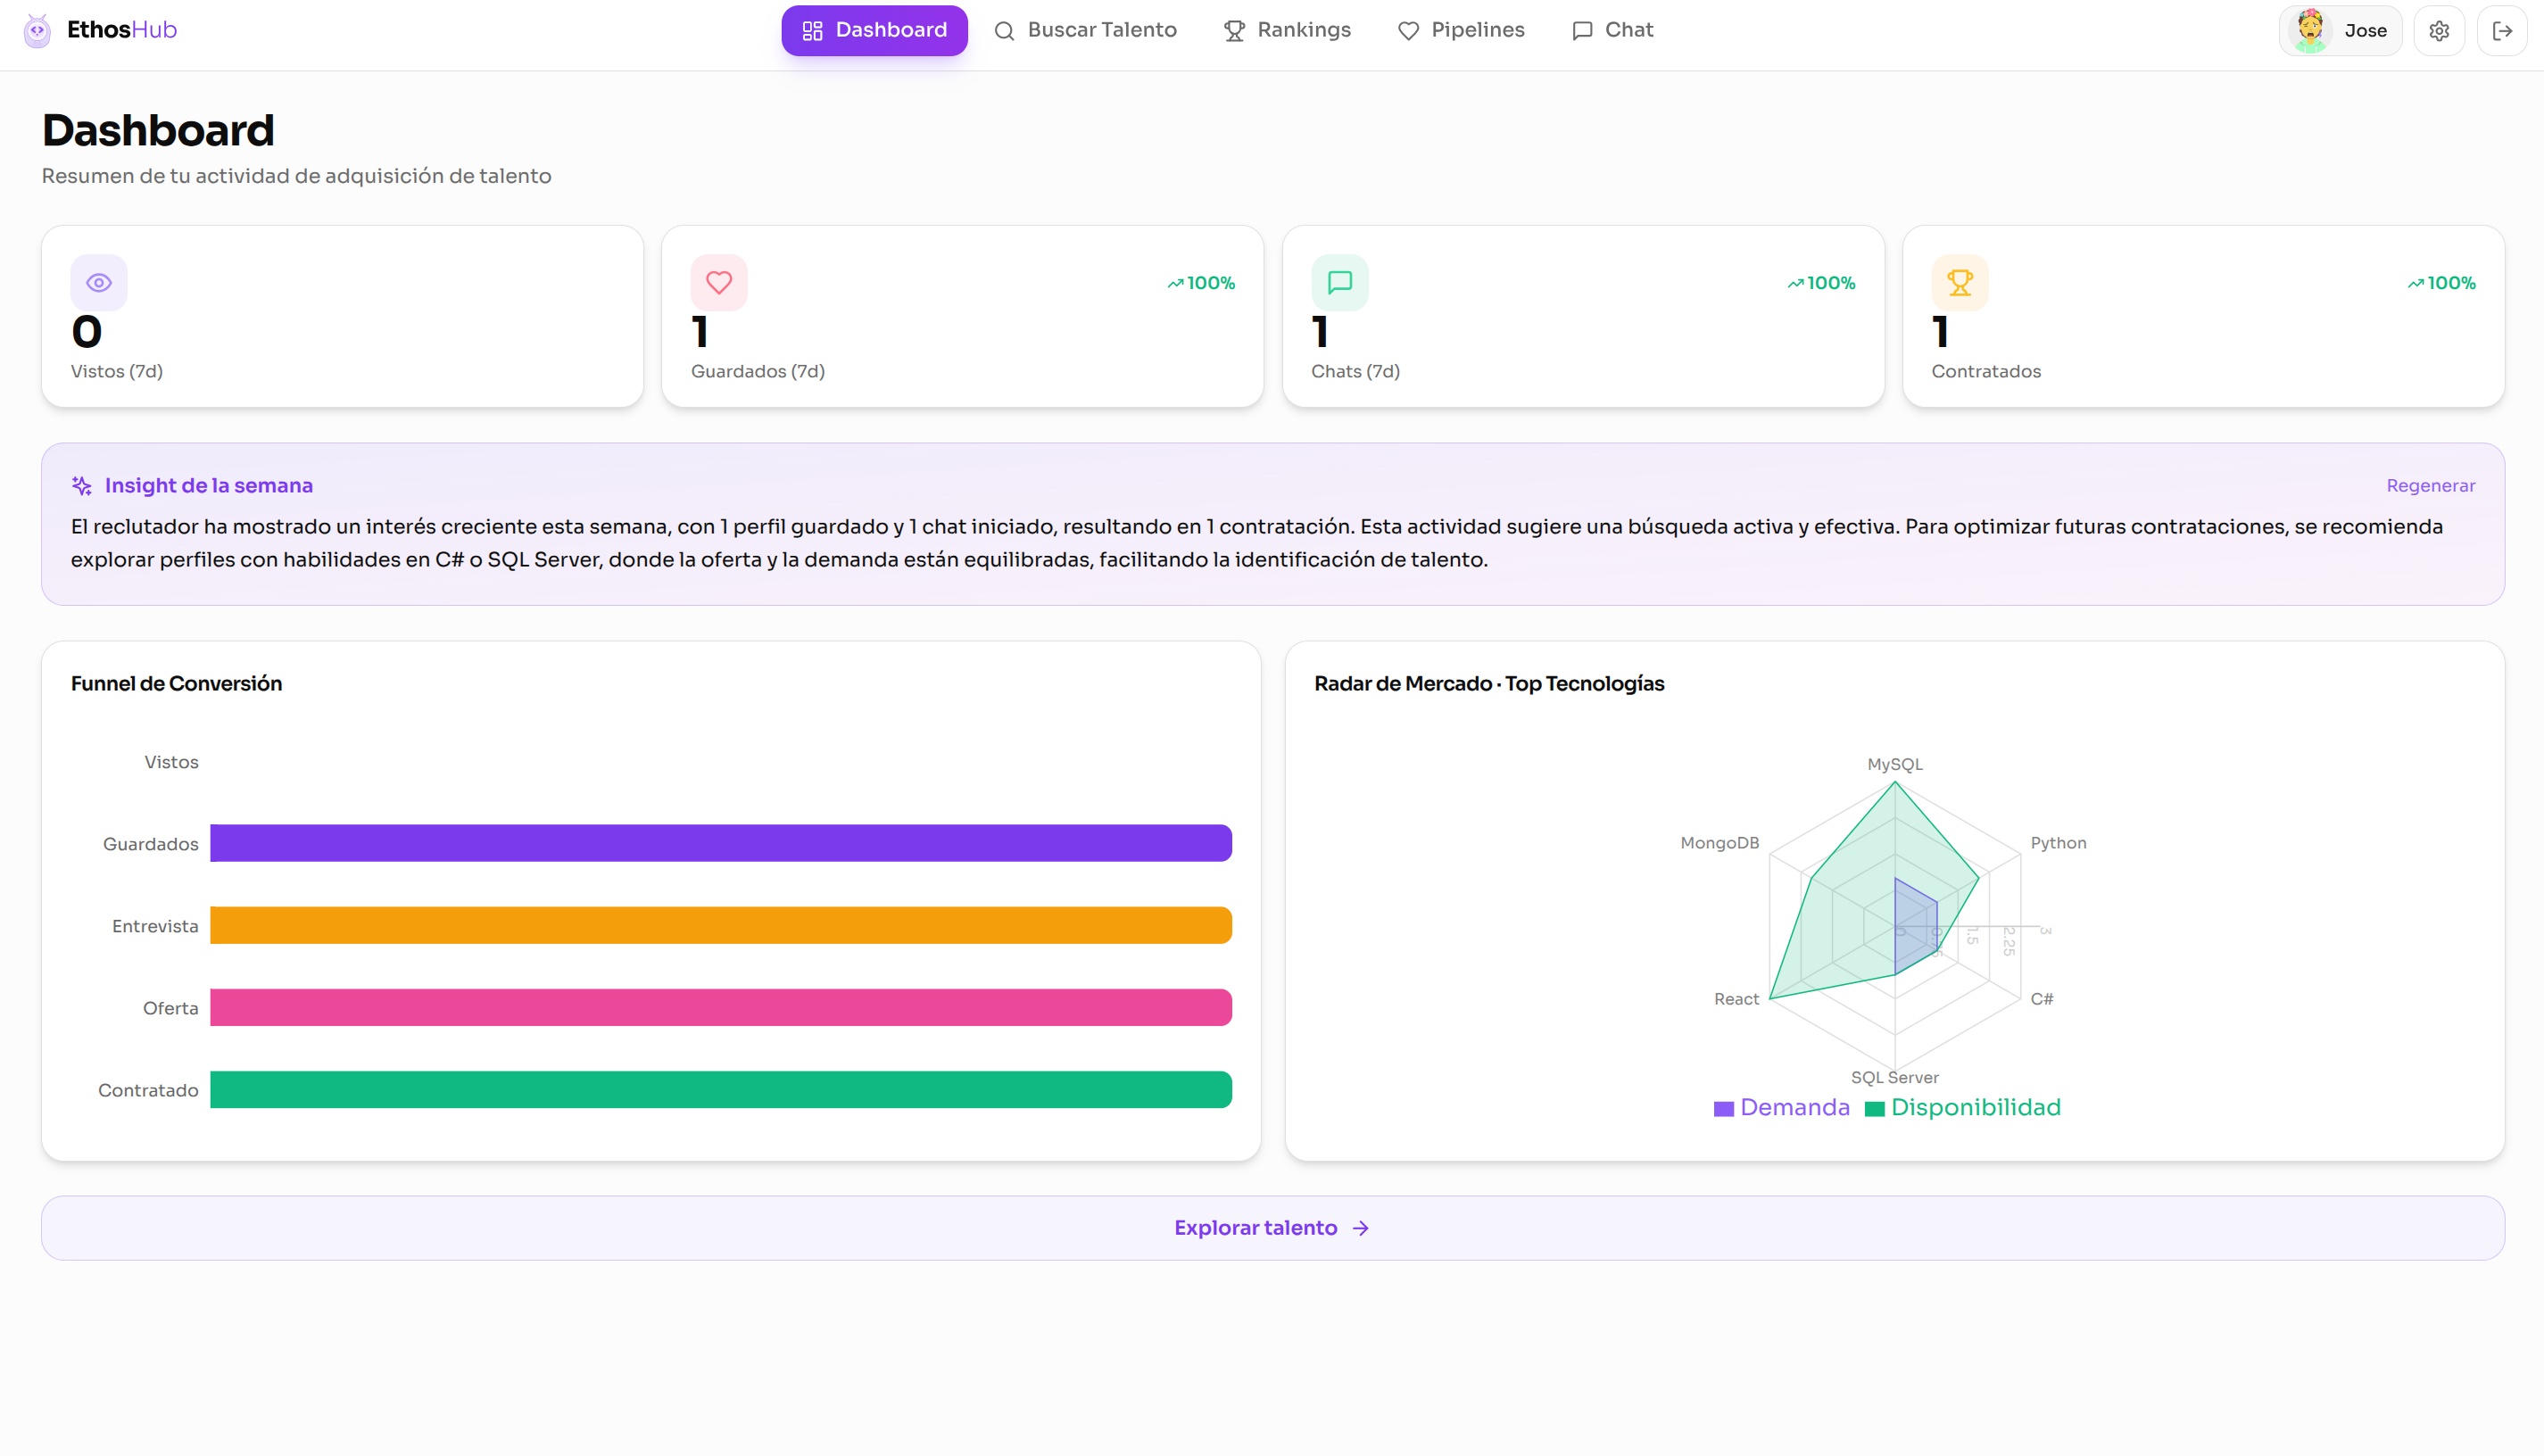
\includegraphics[width=0.7\textwidth]{assets/img/ethoshub/dashboard.png}
    \caption{Dashboard analítico del reclutador (Recharts).}
    \label{fig:s3_dashboard}
\end{figure}

\begin{itemize}[noitemsep]
    \item \textbf{Kanban:} arrastrar y soltar candidatos entre fases del pipeline.
    \item \textbf{Match ring:} indicador visual de afinidad del candidato.
    \item \textbf{Insights IA:} cuatro modos de análisis asistido por Gemini.
    \item \textbf{CV Studio:} edición en Monaco, compilación a PDF y chat con la IA.
\end{itemize}

\subsection{Stores, Servicios y Librerías Avanzadas}
\label{ssec:s3_fe_stores}
Las funcionalidades avanzadas integran las librerías y \textit{stores} de la
tabla~\ref{tab:s3_fe_stores}.

\begin{table}[!ht]
    \centering
    \renewcommand{\arraystretch}{1.3}
    \fontsize{9}{10.8}\selectfont\sffamily
    \begin{tabularx}{\textwidth}{|l|X|}
        \hline
        \rowcolor{colorPrimario}
        \textcolor{white}{\textbf{Elemento}} & \textcolor{white}{\textbf{Responsabilidad}} \\ \hline
        \comando{cvStudioStore} / \comando{cvStudioService} & Documento de CV, asistente IA y compilación. \\ \hline
        \rowcolor{grisTecnico}
        \comando{projectsStore} / \comando{fileService} & Vitrina y subida de evidencias. \\ \hline
        \comando{connectionsStore} & Conexiones URL-first a apps externas. \\ \hline
        \rowcolor{grisTecnico}
        \comando{dashboardService} & Funnel, radar y KPIs del reclutador. \\ \hline
        \comando{@dnd-kit/*} & \textit{Drag \& drop} del pipeline Kanban. \\ \hline
        \rowcolor{grisTecnico}
        Recharts / Leaflet & Gráficas analíticas y mapas. \\ \hline
        Monaco Editor & Editor de código del CV Studio. \\ \hline
        \rowcolor{grisTecnico}
        \comando{@supabase/supabase-js} & Canales Realtime de chat y presencia. \\ \hline
    \end{tabularx}
    \caption{Stores, servicios y librerías de las funcionalidades avanzadas (Sprint 3).}
    \label{tab:s3_fe_stores}
\end{table}

La suscripción a canales Realtime se gestiona en el ciclo de vida del componente: se abre al
montar la vista y se cierra al desmontarla, evitando fugas de \textit{listeners}; la reconexión
preserva la idempotencia descrita en la Sección~\ref{ssec:s3_be_realtime}.

\clearpage

\section{Gestión de la Información (Cumplimiento ISO 26515)}
\label{sec:s3_gestion}

Las funcionalidades concurrentes exigen documentación operativa específica: manuales de monitoreo
(Sección~\ref{ssec:s3_gi_monitoreo}) y guías de resolución de conflictos
(Sección~\ref{ssec:s3_gi_troubleshooting}).\par

\subsection{Manuales de Monitoreo de Servicios en Tiempo Real}
\label{ssec:s3_gi_monitoreo}
Se generaron manuales operativos para el monitoreo de los servicios web en tiempo real (estado de
los canales Realtime, salud de la conexión y latencia), apoyados en Spring Boot Actuator y en el
\comando{HealthController}. La tabla~\ref{tab:s3_monitoreo} resume las señales monitorizadas.

\begin{table}[!ht]
    \centering
    \renewcommand{\arraystretch}{1.3}
    \fontsize{9}{10.8}\selectfont\sffamily
    \begin{tabularx}{\textwidth}{|l|X|}
        \hline
        \rowcolor{colorPrimario}
        \textcolor{white}{\textbf{Señal}} & \textcolor{white}{\textbf{Fuente / criterio}} \\ \hline
        Salud del servicio & \comando{/actuator/health} (UP/DOWN). \\ \hline
        \rowcolor{grisTecnico}
        Estado de canales & Suscripciones Realtime activas vs. esperadas. \\ \hline
        Latencia de IA & Tiempos de respuesta de Gemini y tasa de 429/5xx. \\ \hline
        \rowcolor{grisTecnico}
        Archivos huérfanos & Conteo purgado por el \textit{worker} asíncrono. \\ \hline
    \end{tabularx}
    \caption{Señales de monitoreo de los servicios en tiempo real (Sprint 3).}
    \label{tab:s3_monitoreo}
\end{table}

\subsection{Guías de Troubleshooting de Concurrencia}
\label{ssec:s3_gi_troubleshooting}
Se redactaron guías específicas para la resolución de conflictos derivados de la concurrencia,
recogidas en la tabla~\ref{tab:s3_troubleshooting}.

\begin{table}[!ht]
    \centering
    \renewcommand{\arraystretch}{1.3}
    \fontsize{9}{10.8}\selectfont\sffamily
    \begin{tabularx}{\textwidth}{|X|X|}
        \hline
        \rowcolor{colorPrimario}
        \textcolor{white}{\textbf{Síntoma}} & \textcolor{white}{\textbf{Mitigación}} \\ \hline
        Mensaje duplicado tras reconexión & Idempotencia por clave de deduplicación (V7). \\ \hline
        \rowcolor{grisTecnico}
        Condición de carrera en el pipeline & Mutaciones vía RPC \comando{SECURITY DEFINER} (V8). \\ \hline
        Canal Realtime caído & Reintentos de suscripción con \textit{backoff}. \\ \hline
        \rowcolor{grisTecnico}
        Saturación de IA (429) & Mapeo \comando{AiServiceException} y reintento diferido. \\ \hline
    \end{tabularx}
    \caption{Guía de troubleshooting de concurrencia (Sprint 3).}
    \label{tab:s3_troubleshooting}
\end{table}

La tabla Historias~vs.~Documentación cubrió las Épicas de proyectos, conexiones y reclutador.

\begin{TablaHSDoc}
    EPIC-04 & Vitrina de proyectos & Sí (S3) & Sí (S3) \\ \hline
    EPIC-05 & Conexiones externas & Sí (S3) & Sí (S3) \\ \hline
    EPIC-07 & Reclutador e IA & Sí (S3) & Sí (S3) \\ \hline
\end{TablaHSDoc}

\subsection{Productos de Información del Incremento (ISO 15289)}
\label{ssec:s3_gi_productos}
La tabla~\ref{tab:s3_productos} relaciona los productos de información de las funcionalidades
avanzadas con su artefacto de origen.

\begin{table}[!ht]
    \centering
    \renewcommand{\arraystretch}{1.3}
    \fontsize{9}{10.8}\selectfont\sffamily
    \begin{tabularx}{\textwidth}{|X|X|}
        \hline
        \rowcolor{colorPrimario}
        \textcolor{white}{\textbf{Producto de información}} & \textcolor{white}{\textbf{Artefacto de origen}} \\ \hline
        Manual de monitoreo Realtime & Actuator + \comando{HealthController} + canales. \\ \hline
        \rowcolor{grisTecnico}
        Guía de troubleshooting de concurrencia & RPCs V7/V8 e idempotencia. \\ \hline
        Documentación de RPCs del reclutador & Funciones \comando{SECURITY DEFINER} (V6/V11). \\ \hline
    \end{tabularx}
    \caption{Productos de información del Sprint 3 y su trazabilidad.}
    \label{tab:s3_productos}
\end{table}

\clearpage


% ============================= CAPÍTULO 5 — SPRINT 4 =============================
\setSprint{Sprint 4 - Closed}
\setTag{release/v1.3.0}
\setTaskID{Jira: SPRINT-04}
% =============================================================================
% CAPÍTULO 5 — SPRINT 4: Aseguramiento de Calidad (QA), Pruebas e Integración
% =============================================================================
\chapter{Sprint 4 — Aseguramiento de Calidad, Pruebas e Integración}
\label{cap:sprint4}

El Sprint 4 consolida la calidad del producto: auditoría de la base de datos, refuerzo de
seguridad bajo directrices OWASP, pruebas de extremo a extremo (E2E) y ajustes de
accesibilidad, además de la revisión editorial de toda la documentación.\par

\textbf{Periodo de ejecución:} del lunes 11 al sábado 23 de mayo de 2026 (2 semanas).
\textbf{Módulo entregado (Plan General):} \textit{Visibilidad, Marca Personal y Privacidad}.\par

\section{Cumplimiento de la Definición de Terminado (DoD) y Alcance del Control de Calidad}
\label{sec:s4_resumen}

Cerrado el incremento de funcionalidades avanzadas, el foco se desplaza a la robustez. Se aplica
el DoD definido en la Sección~\ref{ssec:s0_dod} de forma transversal y se mide la deuda técnica.
La tabla~\ref{tab:s4_alcance} resume el alcance del control de calidad.

\begin{table}[!ht]
    \centering
    \renewcommand{\arraystretch}{1.35}
    \fontsize{9}{10.8}\selectfont\sffamily
    \begin{tabularx}{\textwidth}{|l|X|}
        \hline
        \rowcolor{colorPrimario}
        \textcolor{white}{\textbf{Capa}} & \textcolor{white}{\textbf{Actividad de QA}} \\ \hline
        Base de datos & Query profiling, purga de huérfanos y migración de optimización. \\ \hline
        \rowcolor{grisTecnico}
        Backend & Refuerzo OWASP, logging estructurado y telemetría. \\ \hline
        Frontend & Cross-device testing, E2E y accesibilidad. \\ \hline
        \rowcolor{grisTecnico}
        ISO 26515 & Technical review y pruebas de usabilidad de la documentación. \\ \hline
    \end{tabularx}
    \caption{Alcance del Sprint 4 por capa.}
    \label{tab:s4_alcance}
\end{table}

Además de las actividades de QA, el incremento entrega el módulo \textbf{Visibilidad, Marca
Personal y Privacidad} (EPIC-06): ajustes del portafolio público, protección con contraseña,
SEO y políticas de visibilidad, que se aseguran bajo el mismo control de calidad.

\subsection{Objetivos del Incremento}
\label{ssec:s4_objetivos}
\begin{enumerate}[noitemsep]
    \item \textbf{Visibilidad y privacidad:} portafolio público/privado, protección con
    contraseña, SEO y \textit{vanity URL}.
    \item \textbf{Refuerzo OWASP:} \textit{rate limiting}, \textit{blacklist} de JWT,
    sanitización XSS y subida Zero Trust.
    \item \textbf{Calidad de datos:} \textit{query profiling}, purga de huérfanos y migraciones
    de optimización (V11--V15).
    \item \textbf{E2E y accesibilidad:} pruebas de flujos completos, \textit{cross-device} y
    estándares de accesibilidad.
    \item \textbf{Revisión documental:} \textit{technical review} y pruebas de usabilidad de la
    información.
\end{enumerate}

\subsection{Historias de Usuario Abordadas}
\label{ssec:s4_backlog}
\begingroup
\footnotesize
\renewcommand{\arraystretch}{1.35}
\begin{TablaBacklog}
    VIS-01 & Ajustes de portafolio público & Med & 8 & 4 & Visibilidad y SEO configurables. \\ \hline
    VIS-02 & Portafolio con contraseña & Med & 5 & 4 & Bloquea acceso general. \\ \hline
    VIS-03 & Curriculum PDF del portafolio & Med & 5 & 4 & Descarga del CV en PDF. \\ \hline
    IDAR-005 & Panel de administración & Med & 8 & 4 & Métricas y moderación. \\ \hline
    QA-001 & Refuerzo OWASP & Alt & 8 & 4 & Vulnerabilidades mitigadas. \\ \hline
    QA-002 & Pruebas E2E y accesibilidad & Alt & 8 & 4 & Flujos verificados, contraste AA. \\ \hline
\end{TablaBacklog}
\endgroup

\subsection{Ceremonias del Sprint}
\label{ssec:s4_ceremonias}
La tabla~\ref{tab:s4_ceremonias} resume las ceremonias del incremento (11--23 may 2026), centrado
en el aseguramiento de la calidad.

\begin{table}[!ht]
    \centering
    \renewcommand{\arraystretch}{1.3}
    \fontsize{9}{10.8}\selectfont\sffamily
    \begin{tabularx}{\textwidth}{|l|X|}
        \hline
        \rowcolor{colorPrimario}
        \textcolor{white}{\textbf{Ceremonia}} & \textcolor{white}{\textbf{Resultado}} \\ \hline
        Planning & Plan de QA, OWASP, E2E y módulo de visibilidad. \\ \hline
        \rowcolor{grisTecnico}
        Daily & Seguimiento de defectos y deuda técnica. \\ \hline
        Review & Demostración del refuerzo de seguridad y accesibilidad. \\ \hline
        \rowcolor{grisTecnico}
        Retrospective & Cierre del \textit{carry-over} del Sprint 3. \\ \hline
    \end{tabularx}
    \caption{Ceremonias Scrum del Sprint 4.}
    \label{tab:s4_ceremonias}
\end{table}

\clearpage

\section{Base de Datos: Auditoría de Rendimiento y Consistencia}
\label{sec:s4_database}

La auditoría de la base de datos persigue dos metas: optimizar el rendimiento de las consultas
críticas y garantizar la consistencia tras la introducción de las funcionalidades de visibilidad
del portafolio. La Figura~\ref{fig:s4_profiling} resume el ciclo de \textit{query profiling}.\par

\begin{figure}[!ht]
    \centering
    \begin{tikzpicture}[
        node distance=0.6cm,
        s/.style={draw=colorPrimario, fill=headerTabla, thick, rounded corners=2pt,
            text width=2.4cm, align=center, minimum height=1.0cm, font=\sffamily\scriptsize},
        rel/.style={-{Latex[length=2mm]}, colorPrimario, font=\sffamily\tiny}
    ]
        \node[s] (a) {1. EXPLAIN\\ANALYZE};
        \node[s, right=of a] (b) {2. Detecta\\seq scans};
        \node[s, right=of b] (c) {3. Crea\\índice};
        \node[s, right=of c] (d) {4. Verifica\\mejora};
        \draw[rel] (a)--(b); \draw[rel] (b)--(c); \draw[rel] (c)--(d);
        \draw[rel, dashed] (d.south) to[bend left=25] (a.south);
    \end{tikzpicture}
    \caption{Ciclo de \textit{Query Profiling} aplicado en el Sprint 4.}
    \label{fig:s4_profiling}
\end{figure}

\subsection{Análisis de Planes de Ejecución y Remoción de Huérfanos}
\label{ssec:s4_db_profiling}
Se analizaron los planes de ejecución (\textit{Query Profiling}) de las consultas críticas para
detectar escaneos costosos, y se removieron registros huérfanos. Un \textit{worker} asíncrono del
backend purga periódicamente los archivos físicos sin referencia en el modelo relacional,
liberando almacenamiento y preservando la integridad referencial.

\begin{itemize}[noitemsep]
    \item \textbf{Planes de ejecución:} \comando{EXPLAIN ANALYZE} sobre listados de talento y mensajería.
    \item \textbf{Huérfanos:} archivos sin fila asociada eliminados por el \textit{worker}.
    \item \textbf{Consistencia:} verificación de claves foráneas y políticas RLS tras cada migración.
\end{itemize}

\subsection{Scripts de Migración de Optimización Final}
\label{ssec:s4_db_migracion}
Se aplicaron migraciones de optimización y corrección, resumidas en la
tabla~\ref{tab:s4_migraciones}.

\begin{table}[!ht]
    \centering
    \renewcommand{\arraystretch}{1.3}
    \fontsize{9}{10.8}\selectfont\sffamily
    \begin{tabularx}{\textwidth}{|l|X|}
        \hline
        \rowcolor{colorPrimario}
        \textcolor{white}{\textbf{Migración}} & \textcolor{white}{\textbf{Contenido}} \\ \hline
        \comando{V11} & Fix de RPCs de chat/perfil + wrapper de talent-views. \\ \hline
        \rowcolor{grisTecnico}
        \comando{V12} & Trigger de sync de email a \comando{profiles\_basic}/\comando{profiles\_company}. \\ \hline
        \comando{V13} & Tabla de solicitudes de cambio de email. \\ \hline
        \rowcolor{grisTecnico}
        \comando{V15} & Política de SELECT para likes de perfil. \\ \hline
    \end{tabularx}
    \caption{Migraciones de optimización y corrección (Sprint 4).}
    \label{tab:s4_migraciones}
\end{table}

\begin{NotaTecnica}
La migración V15 introduce una política RLS de \comando{SELECT} para los \textit{likes} de
perfil, permitiendo que el dueño consulte quién valoró su portafolio sin exponer datos de
terceros, manteniendo el aislamiento por usuario.
\end{NotaTecnica}

\clearpage
\subsection{Sincronización de Email y Solicitudes de Cambio}
\label{ssec:s4_db_email}
Las migraciones V12 y V13 endurecen el cambio de email. Un \textit{trigger} propaga el cambio
confirmado en \comando{auth.users} a las tablas de perfil, y una tabla registra las solicitudes
pendientes hasta su confirmación.

\begin{lstlisting}[language=SQL, caption={Trigger de sincronización de email (V12).}, label={lst:s4_trigger}]
CREATE TRIGGER on_auth_email_changed
  AFTER UPDATE OF email ON auth.users
  FOR EACH ROW WHEN (OLD.email IS DISTINCT FROM NEW.email)
  EXECUTE FUNCTION core.sync_auth_email_to_profiles();
\end{lstlisting}

\begin{table}[!ht]
    \centering
    \renewcommand{\arraystretch}{1.25}
    \fontsize{8.8}{10.5}\selectfont\sffamily
    \begin{tabularx}{\textwidth}{|l|l|X|}
        \hline
        \rowcolor{colorPrimario}
        \textcolor{white}{\textbf{Columna}} & \textcolor{white}{\textbf{Tipo}} & \textcolor{white}{\textbf{Propósito}} \\ \hline
        \comando{auth\_id} & \comando{uuid} & Usuario solicitante. \\ \hline
        \rowcolor{grisTecnico}
        \comando{new\_email} & \comando{text} & Correo propuesto. \\ \hline
        \comando{token\_hash} & \comando{text} unique & \textit{Hash} del enlace de confirmación. \\ \hline
        \rowcolor{grisTecnico}
        \comando{consumed} & \comando{boolean} & Marca de consumo. \\ \hline
        \comando{expires\_at} & \comando{timestamptz} & Vencimiento de la solicitud. \\ \hline
    \end{tabularx}
    \caption{Columnas de \comando{core.email\_change\_requests} (V13).}
    \label{tab:s4_email_cols}
\end{table}

La tabla \comando{email\_change\_requests} tiene RLS activo \textbf{sin políticas}: solo el
backend (rol de servicio) la manipula, evitando cualquier exposición directa al cliente.

\clearpage

\section{Backend: Refactorización, Seguridad Avanzada y Pruebas de Carga}
\label{sec:s4_backend}

El backend se endurece bajo directrices OWASP y se entrega el módulo de visibilidad del
portafolio. La Figura~\ref{fig:s4_owasp} resume las capas de mitigación incorporadas al
\comando{SecurityConfig}.\par

\begin{figure}[!ht]
    \centering
    \begin{tikzpicture}[
        node distance=0.45cm,
        m/.style={draw=colorPrimario, fill=headerTabla, thick, rounded corners=2pt,
            text width=2.3cm, align=center, minimum height=1.1cm, font=\sffamily\scriptsize},
        rel/.style={-{Latex[length=2mm]}, colorPrimario}
    ]
        \node[m] (a) {Rate\\Limiting};
        \node[m, right=of a] (b) {JWT\\Blacklist};
        \node[m, right=of b] (c) {Sanitización\\XSS};
        \node[m, right=of c] (d) {Zero Trust\\Upload};
        \draw[rel] (a)--(b); \draw[rel] (b)--(c); \draw[rel] (c)--(d);
    \end{tikzpicture}
    \caption{Capas de mitigación OWASP del Sprint 4.}
    \label{fig:s4_owasp}
\end{figure}

\subsection{Mitigación de Vulnerabilidades (OWASP) y Deuda Técnica}
\label{ssec:s4_be_owasp}
Se reforzó el \comando{SecurityConfig} con un conjunto de mitigaciones alineadas a OWASP, y se
optimizaron los tiempos de respuesta. Se entregaron además los controladores de visibilidad
\comando{PortfolioSettingsController} y \comando{PortfolioPublicController} (vista pública con o
sin contraseña). Las principales medidas de seguridad se listan a continuación.

\begin{itemize}[noitemsep]
    \item \textbf{Rate limiting:} freno a ataques de fuerza bruta en autenticación.
    \item \textbf{Blacklist de JWT:} el \comando{JwtAuthenticationFilter} valida cada token
    contra una lista negra, garantizando un cierre de sesión real.
    \item \textbf{Sanitización XSS:} limpieza estricta de campos de texto (título, descripción).
    \item \textbf{Subida Zero Trust:} verificación de \textit{magic numbers}, prevención de
    \textit{path traversal} y \\ \comando{Content-Disposition: attachment} en descargas.
    \item \textbf{Portafolio protegido:} acceso público condicionado a contraseña cuando el
    perfil así lo configura.
\end{itemize}

\begin{AlertaDefecto}
Se detectó que las extensiones reportadas por el cliente no son fiables; la mitigación analiza
las cabeceras binarias del archivo para determinar su auténtico tipo MIME antes de aceptarlo.
\end{AlertaDefecto}

\subsection{Logging Estructurado, Auditoría y Telemetría}
\label{ssec:s4_be_telemetria}
Se configuró \textit{logging} estructurado, auditoría interna y herramientas de telemetría para
observabilidad. La gestión de errores de IA se centraliza en \comando{AiServiceException},
mapeando los fallos upstream de Gemini sin exponer 500 genéricos. Las señales de observabilidad
monitorizadas se resumen en la tabla~\ref{tab:s4_observabilidad}.

\begin{table}[!ht]
    \centering
    \renewcommand{\arraystretch}{1.3}
    \fontsize{9}{10.8}\selectfont\sffamily
    \begin{tabularx}{\textwidth}{|l|X|}
        \hline
        \rowcolor{colorPrimario}
        \textcolor{white}{\textbf{Señal}} & \textcolor{white}{\textbf{Fuente / uso}} \\ \hline
        Logs estructurados & Trazas por petición con identificador de correlación. \\ \hline
        \rowcolor{grisTecnico}
        Métricas Actuator & Latencia, errores y uso de recursos. \\ \hline
        Salud del servicio & \comando{/actuator/health} (UP/DOWN). \\ \hline
        \rowcolor{grisTecnico}
        Auditoría de seguridad & Intentos de acceso y eventos OWASP. \\ \hline
        Errores de IA & Tasa de 429/5xx mapeada por \comando{AiServiceException}. \\ \hline
    \end{tabularx}
    \caption{Señales de observabilidad y telemetría (Sprint 4).}
    \label{tab:s4_observabilidad}
\end{table}

La tabla~\ref{tab:s4_owasp_map} relaciona cada categoría OWASP con su control.

\begin{table}[!ht]
    \centering
    \renewcommand{\arraystretch}{1.3}
    \fontsize{9}{10.8}\selectfont\sffamily
    \begin{tabularx}{\textwidth}{|l|X|}
        \hline
        \rowcolor{colorPrimario}
        \textcolor{white}{\textbf{Riesgo OWASP}} & \textcolor{white}{\textbf{Control implementado}} \\ \hline
        Control de acceso roto & RLS + RBAC \comando{AdminEmailPolicy}. \\ \hline
        \rowcolor{grisTecnico}
        Inyección & Sanitización XSS y validación Jakarta. \\ \hline
        Fallos de identificación & \textit{Blacklist} de JWT y rate limiting. \\ \hline
        \rowcolor{grisTecnico}
        Carga de archivos insegura & Verificación \textit{magic number} + anti path-traversal. \\ \hline
    \end{tabularx}
    \caption{Mapeo de riesgos OWASP a controles del backend (Sprint 4).}
    \label{tab:s4_owasp_map}
\end{table}

\subsection{Gestión de la Deuda Técnica}
\label{ssec:s4_be_deuda}
El control de calidad incluyó la reducción sistemática de la deuda técnica acumulada en los
incrementos previos, priorizada por impacto en seguridad y rendimiento, según la
tabla~\ref{tab:s4_deuda}.

\begin{table}[!ht]
    \centering
    \renewcommand{\arraystretch}{1.3}
    \fontsize{9}{10.8}\selectfont\sffamily
    \begin{tabularx}{\textwidth}{|X|l|X|}
        \hline
        \rowcolor{colorPrimario}
        \textcolor{white}{\textbf{Deuda}} & \textcolor{white}{\textbf{Prioridad}} & \textcolor{white}{\textbf{Resolución}} \\ \hline
        RPCs sin \comando{search\_path} fijado & Alta & Bloqueo del esquema en V11. \\ \hline
        \rowcolor{grisTecnico}
        Desfase de email auth$\to$perfil & Alta & Trigger de sincronización (V12). \\ \hline
        Consultas con \textit{seq scan} & Media & Índices estratégicos. \\ \hline
        \rowcolor{grisTecnico}
        Archivos huérfanos & Media & \textit{Worker} de purga asíncrona. \\ \hline
        \textit{Carry-over} de concurrencia (S3) & Media & Cierre con RPCs seguras de pipeline. \\ \hline
    \end{tabularx}
    \caption{Deuda técnica gestionada en el Sprint 4.}
    \label{tab:s4_deuda}
\end{table}

\subsection{Diagrama de Secuencia: Petición Protegida (Rate Limit + Blacklist)}
\label{ssec:s4_seq_owasp}
La Figura~\ref{fig:s4_seq} muestra cómo una petición atraviesa el control de tasa y la
verificación de \textit{blacklist} de JWT antes de alcanzar el controlador.

\begin{figure}[!ht]
    \centering
    \begin{tikzpicture}[font=\sffamily\scriptsize, >=Latex,
        part/.style={draw=colorPrimario, fill=headerTabla, rounded corners=2pt,
            minimum height=0.6cm, text width=2.1cm, align=center},
        msg/.style={-{Latex[length=1.6mm]}, colorPrimario},
        ret/.style={-{Latex[length=1.6mm]}, dashed, grisISO}]
        \node[part] (c)  at (0,0)    {Cliente};
        \node[part] (rl) at (3.8,0)  {Rate Limiter};
        \node[part] (jf) at (7.8,0)  {JwtAuthFilter};
        \node[part] (ct) at (11.6,0) {Controller};
        \foreach \n in {c,rl,jf,ct} \draw[grisISO, dashed] (\n.south) -- ++(0,-5.0);
        \draw[msg] (0,-0.9)    -- node[above]{1. request} (3.8,-0.9);
        \draw[msg] (3.8,-1.7)  -- node[above]{2. dentro de cuota} (7.8,-1.7);
        \draw[msg] (7.8,-2.5)  -- ++(0.7,0) -- ++(0,-0.5) -- node[below,xshift=2pt]{3. token en blacklist?} ++(-0.7,0);
        \draw[msg] (7.8,-3.5)  -- node[above]{4. JWT válido} (11.6,-3.5);
        \draw[ret] (11.6,-4.3) -- node[above]{5. 200 / 401 / 429} (0,-4.3);
    \end{tikzpicture}
    \caption{Diagrama de secuencia de una petición protegida (rate limit y blacklist).}
    \label{fig:s4_seq}
\end{figure}

\clearpage

\section{Frontend: Pruebas de Extremo a Extremo (E2E) y Accesibilidad}
\label{sec:s4_frontend}

El frontend entrega las vistas de visibilidad y privacidad del portafolio y se somete a un
control de calidad exhaustivo: \textit{cross-device}, flujos E2E y accesibilidad. La
Figura~\ref{fig:s4_visibilidad} muestra el panel de ajustes de visibilidad.\par

\begin{figure}[!ht]
    \centering
    \fbox{\begin{minipage}[c][4.0cm][c]{0.62\textwidth}
        \centering
        \sffamily\color{grisISO}\footnotesize
        [\,Captura de pantalla pendiente\,]\par
        \vspace{0.3cm}
        Ajustes de visibilidad, SEO y protección con contraseña del portafolio\par
        \vspace{0.2cm}
        \tiny(reemplazar por \texttt{assets/img/screenshots/visibilidad.png})
    \end{minipage}}
    \caption{Panel de visibilidad y privacidad del portafolio.}
    \label{fig:s4_visibilidad}
\end{figure}

\subsection{Inconsistencias Visuales y Cross-device Testing}
\label{ssec:s4_fe_crossdevice}
Se resolvieron inconsistencias visuales en distintas pantallas y resoluciones mediante
\textit{cross-device testing}, garantizando una adaptación fluida sin desbordamientos en móvil,
tableta y escritorio. La tabla~\ref{tab:s4_breakpoints} resume los \textit{breakpoints} verificados.

\begin{table}[!ht]
    \centering
    \renewcommand{\arraystretch}{1.3}
    \fontsize{9}{10.8}\selectfont\sffamily
    \begin{tabularx}{\textwidth}{|l|l|X|}
        \hline
        \rowcolor{colorPrimario}
        \textcolor{white}{\textbf{Dispositivo}} & \textcolor{white}{\textbf{Ancho}} & \textcolor{white}{\textbf{Verificación}} \\ \hline
        Móvil & 360--430\,px & Sidebar visible; sin scroll horizontal. \\ \hline
        \rowcolor{grisTecnico}
        Tableta & 768--1024\,px & Reflujo de columnas; tablas responsivas. \\ \hline
        Escritorio & $\geq$1280\,px & Sidebar oculto; layout completo. \\ \hline
    \end{tabularx}
    \caption{Breakpoints verificados en el cross-device testing (Sprint 4).}
    \label{tab:s4_breakpoints}
\end{table}

\subsection{Flujos Completos y Estándares de Accesibilidad}
\label{ssec:s4_fe_accesibilidad}
Se simularon automatizadamente flujos completos de navegación del perfil (Vitest + Testing
Library, entorno jsdom) y se verificaron los estándares de accesibilidad: contraste de color,
navegación por teclado y etiquetado semántico.

\begin{TablaCasoPrueba}
    1 & Navegación login-dashboard por teclado & Foco visible y orden lógico & \estadoPass \\ \hline
    2 & Contraste de texto sobre fondo primario & Cumple ratio AA (4.5:1) & \estadoPass \\ \hline
    3 & Render en viewport de 360px & Sin scroll horizontal ni cortes & \estadoPass \\ \hline
    4 & Portafolio protegido sin contraseña & Acceso bloqueado correctamente & \estadoPass \\ \hline
\end{TablaCasoPrueba}

\subsection{Herramientas y Criterios de Accesibilidad}
\label{ssec:s4_fe_a11y}
La verificación de accesibilidad se apoya en los criterios de la tabla~\ref{tab:s4_a11y},
alineados con las pautas WCAG nivel AA.

\begin{table}[!ht]
    \centering
    \renewcommand{\arraystretch}{1.3}
    \fontsize{9}{10.8}\selectfont\sffamily
    \begin{tabularx}{\textwidth}{|l|X|}
        \hline
        \rowcolor{colorPrimario}
        \textcolor{white}{\textbf{Criterio}} & \textcolor{white}{\textbf{Verificación}} \\ \hline
        Contraste & Ratio $\geq$ 4.5:1 en texto normal (AA). \\ \hline
        \rowcolor{grisTecnico}
        Navegación por teclado & Orden de foco lógico y foco visible. \\ \hline
        Etiquetado semántico & Roles ARIA y etiquetas en formularios. \\ \hline
        \rowcolor{grisTecnico}
        Movimiento reducido & Respeto de \comando{prefers-reduced-motion}. \\ \hline
        Responsividad & Sin scroll horizontal en 360--1280\,px. \\ \hline
    \end{tabularx}
    \caption{Criterios de accesibilidad verificados (Sprint 4).}
    \label{tab:s4_a11y}
\end{table}

Las pruebas automatizadas (Vitest + Testing Library, \comando{jsdom}) simulan flujos completos de
navegación; los hallazgos de contraste y foco se resolvieron antes del cierre del incremento,
conforme al DoD de la Sección~\ref{ssec:s0_dod}.

\clearpage

\section{Gestión de la Información (Cumplimiento ISO 26515)}
\label{sec:s4_gestion}

\subsection{Revisión Editorial y de Precisión Técnica}
\label{ssec:s4_gi_review}
Se ejecutó una revisión editorial y de precisión técnica (\textit{Technical Review}) de toda la
documentación recopilada, corrigiendo inconsistencias terminológicas y verificando que cada
afirmación tuviera respaldo en un artefacto real del código.

\subsection{Pruebas de Usabilidad de la Información}
\label{ssec:s4_gi_usabilidad}
Se realizaron pruebas de usabilidad de la información, confirmando que manuales y diagramas
describen exactamente el estado actual del producto. La tabla Historias~vs.~Documentación cubrió
las Épicas de administración y UX.

\begin{TablaHSDoc}
    EPIC-07 & Panel de administración & Sí (S4) & Sí (S4) \\ \hline
    EPIC-08 & UX y diseño adaptable & Sí (S4) & Sí (S4) \\ \hline
\end{TablaHSDoc}

\subsection{Productos de Información del Incremento (ISO 15289)}
\label{ssec:s4_gi_productos}
La tabla~\ref{tab:s4_productos} relaciona los productos de información del control de calidad con
su artefacto de origen.

\begin{table}[!ht]
    \centering
    \renewcommand{\arraystretch}{1.3}
    \fontsize{9}{10.8}\selectfont\sffamily
    \begin{tabularx}{\textwidth}{|X|X|}
        \hline
        \rowcolor{colorPrimario}
        \textcolor{white}{\textbf{Producto de información}} & \textcolor{white}{\textbf{Artefacto de origen}} \\ \hline
        Informe de \textit{technical review} & Revisión editorial de toda la documentación. \\ \hline
        \rowcolor{grisTecnico}
        Catálogo de casos E2E & Suite Vitest + Testing Library (Anexo~\ref{cap:anexo_e2e}). \\ \hline
        Matriz de controles OWASP & \comando{SecurityConfig} y filtros del Sprint 4. \\ \hline
    \end{tabularx}
    \caption{Productos de información del Sprint 4 y su trazabilidad.}
    \label{tab:s4_productos}
\end{table}

\clearpage


% ============================= CAPÍTULO 6 — SPRINT 5 =============================
\setSprint{Sprint 5 - Closed}
\setTag{release/v2.0.0}
\setTaskID{Jira: SPRINT-05}
% =============================================================================
% CAPÍTULO 6 — SPRINT 5: Despliegue, Empaquetado y Cierre de Versión
% =============================================================================
\chapter{Sprint 5 — Despliegue, Empaquetado y Cierre de Versión}
\label{cap:sprint5}

El Sprint 5 cierra la versión 2.0.0 del producto: preparación de la base de datos para
producción, despliegue de los servicios e infraestructura, compilación optimizada del frontend y
publicación de las Release Notes integrales.\par

\textbf{Periodo de ejecución:} del lunes 25 de mayo al sábado 6 de junio de 2026 (2 semanas).
\textbf{Módulo entregado (Plan General):} \textit{Estadísticas, Adaptabilidad y Lanzamiento}.\par

\section{Plan Estratégico de Lanzamiento (Release Plan)}
\label{sec:s5_resumen}

El plan de lanzamiento coordina las cuatro capas hacia un único artefacto monolítico
desplegable. La tabla~\ref{tab:s5_alcance} resume las actividades por capa.

\begin{table}[!ht]
    \centering
    \renewcommand{\arraystretch}{1.35}
    \fontsize{9}{10.8}\selectfont\sffamily
    \begin{tabularx}{\textwidth}{|l|X|}
        \hline
        \rowcolor{colorPrimario}
        \textcolor{white}{\textbf{Capa}} & \textcolor{white}{\textbf{Actividad de lanzamiento}} \\ \hline
        Base de datos & Seeders de datos maestros y políticas de backups. \\ \hline
        \rowcolor{grisTecnico}
        Backend & Variables de entorno seguras y despliegue en contenedores. \\ \hline
        Frontend & Build optimizado, code splitting y distribución de assets. \\ \hline
        \rowcolor{grisTecnico}
        ISO 26515 & Release Notes y empaquetado de la base de conocimiento. \\ \hline
    \end{tabularx}
    \caption{Alcance del Sprint 5 por capa.}
    \label{tab:s5_alcance}
\end{table}

El módulo del Plan General para este cierre es \textbf{Estadísticas, Adaptabilidad y
Lanzamiento}: paneles de métricas para el profesional y el administrador, adaptación final a
móvil, cambio de idioma y modo claro/oscuro, y el despliegue productivo del artefacto monolítico.

\subsection{Objetivos del Incremento}
\label{ssec:s5_objetivos}
\begin{enumerate}[noitemsep]
    \item \textbf{Estadísticas:} dashboards de métricas y reportes para profesional y administrador.
    \item \textbf{Adaptabilidad:} i18n (es/en/pt), modo claro/oscuro y responsividad final.
    \item \textbf{Producción de datos:} \textit{seeders} maestros y políticas de \textit{backups}.
    \item \textbf{Despliegue:} empaquetado monolítico, contenedores y variables seguras.
    \item \textbf{Cierre de versión:} Release Notes 2.0.0 y empaquetado de la base de conocimiento.
\end{enumerate}

\subsection{Historias de Usuario Abordadas}
\label{ssec:s5_backlog}
\begingroup
\footnotesize
\renewcommand{\arraystretch}{1.35}
\begin{TablaBacklog}
    IDAR-002 & Dashboard de métricas (admin) & Med & 8 & 5 & Visión general de la plataforma. \\ \hline
    UX-002 & Cambio de idioma (i18n) & Med & 5 & 5 & Traducción sin recarga (es/en/pt). \\ \hline
    UX-005 & Modo claro/oscuro & Med & 3 & 5 & Cambio de tema persistente. \\ \hline
    REL-001 & Despliegue monolítico & Alt & 8 & 5 & JAR único FE+BE en producción. \\ \hline
    REL-002 & Backups y recuperación & Alt & 5 & 5 & Política automatizada de respaldos. \\ \hline
    REL-003 & Release Notes 2.0.0 & Med & 3 & 5 & Notas de versión publicadas. \\ \hline
\end{TablaBacklog}
\endgroup

\subsection{Ceremonias del Sprint}
\label{ssec:s5_ceremonias}
La tabla~\ref{tab:s5_ceremonias} resume las ceremonias del incremento de cierre
(25 may--6 jun 2026), incluida la \textit{Sprint Review} de fin de versión.

\begin{table}[!ht]
    \centering
    \renewcommand{\arraystretch}{1.3}
    \fontsize{9}{10.8}\selectfont\sffamily
    \begin{tabularx}{\textwidth}{|l|X|}
        \hline
        \rowcolor{colorPrimario}
        \textcolor{white}{\textbf{Ceremonia}} & \textcolor{white}{\textbf{Resultado}} \\ \hline
        Planning & Plan de lanzamiento, seeders, despliegue y métricas. \\ \hline
        \rowcolor{grisTecnico}
        Daily & Coordinación del empaquetado y la contenerización. \\ \hline
        Review (versión) & Demostración del despliegue 2.0.0 al cliente. \\ \hline
        \rowcolor{grisTecnico}
        Retrospective & Cierre del proyecto y lecciones aprendidas. \\ \hline
    \end{tabularx}
    \caption{Ceremonias Scrum del Sprint 5 (cierre de versión).}
    \label{tab:s5_ceremonias}
\end{table}

\clearpage

\section{Base de Datos: Preparación para Entornos de Producción}
\label{sec:s5_database}

La preparación para producción combina la siembra de datos maestros y una política de respaldos
automatizada. La Figura~\ref{fig:s5_backup} resume el ciclo de respaldo y recuperación sobre
la base de datos PostgreSQL~15.10 autoalojada en el servidor TIS.\par

\begin{figure}[!ht]
    \centering
    \begin{tikzpicture}[
        node distance=0.6cm,
        s/.style={draw=colorPrimario, fill=headerTabla, thick, rounded corners=2pt,
            text width=2.4cm, align=center, minimum height=1.0cm, font=\sffamily\scriptsize},
        rel/.style={-{Latex[length=2mm]}, colorPrimario, font=\sffamily\tiny}
    ]
        \node[s] (a) {1. Backup\\programado};
        \node[s, right=of a] (b) {2. Almacén\\seguro};
        \node[s, right=of b] (c) {3. Verifica\\integridad};
        \node[s, right=of c] (d) {4. Restaura\\(contingencia)};
        \draw[rel] (a)--(b); \draw[rel] (b)--(c); \draw[rel] (c)--(d);
    \end{tikzpicture}
    \caption{Ciclo de respaldo y recuperación de datos (Sprint 5).}
    \label{fig:s5_backup}
\end{figure}

\subsection{Inyección de Semillas de Datos Maestros (Seeders)}
\label{ssec:s5_db_seeders}
Se inyectaron las semillas de datos maestros requeridas para el arranque operativo: catálogos
base, configuraciones por defecto y datos de referencia, garantizando que el sistema sea
funcional desde el primer despliegue.

\subsection{Políticas de Respaldos y Recuperación}
\label{ssec:s5_db_backups}
Se implementaron políticas automatizadas de respaldos (\textit{backups}) sobre la base de datos
PostgreSQL~15.10 (volcados con \comando{pg\_dump}) y protocolos de recuperación ante
contingencias, definiendo la frecuencia de copia y el procedimiento de restauración.

\begin{NotaTecnica}
Las migraciones se aplican sobre PostgreSQL~15.10 de forma controlada a través del cliente web
phpPgAdmin (\url{http://bytebusters.tis.cs.umss.edu.bo/phppgadmin}); cada script se revisa antes
de ejecutarlo en un entorno compartido para preservar la integridad del schema \comando{core}.
\end{NotaTecnica}

\subsection{Catálogo de Semillas y Política de Respaldos}
\label{ssec:s5_db_catalogo}
La tabla~\ref{tab:s5_seeds} resume los datos maestros sembrados y la política de respaldos
aplicada para el arranque operativo.

\begin{table}[!ht]
    \centering
    \renewcommand{\arraystretch}{1.3}
    \fontsize{9}{10.8}\selectfont\sffamily
    \begin{tabularx}{\textwidth}{|l|X|}
        \hline
        \rowcolor{colorPrimario}
        \textcolor{white}{\textbf{Elemento}} & \textcolor{white}{\textbf{Contenido / criterio}} \\ \hline
        \comando{global\_skill\_tags} & Catálogo base de \textit{skills} con categorías. \\ \hline
        \rowcolor{grisTecnico}
        Cuentas administrativas & Semilla de cuentas \comando{adm.*@ethoshub.dev}. \\ \hline
        Configuración por defecto & Valores iniciales de \comando{portfolio\_settings}. \\ \hline
        \rowcolor{grisTecnico}
        Respaldo programado & Copia periódica con \comando{pg\_dump} del servidor TIS. \\ \hline
        Verificación de integridad & Comprobación del respaldo antes de archivarlo. \\ \hline
        \rowcolor{grisTecnico}
        Recuperación & Procedimiento de restauración ante contingencia. \\ \hline
    \end{tabularx}
    \caption{Semillas maestras y política de respaldos (Sprint 5).}
    \label{tab:s5_seeds}
\end{table}

El ciclo completo de respaldo y recuperación se modela en la Figura~\ref{fig:s5_backup},
garantizando la continuidad operativa ante incidentes en producción.

\clearpage

\section{Backend: Despliegue de Servicios e Infraestructura Productiva}
\label{sec:s5_backend}

El despliegue productivo materializa la arquitectura monolítica fijada en el Sprint 0
(Sección~\ref{ssec:s0_c4_contenedores}): un único JAR que sirve la API y la SPA, ejecutado en
contenedores. La Figura~\ref{fig:s5_deploy} muestra la topología de despliegue.\par

\begin{figure}[!ht]
    \centering
    \begin{tikzpicture}[
        node distance=0.8cm and 1.2cm,
        box/.style={draw=colorPrimario, fill=headerTabla, thick, rounded corners=2pt,
            text width=2.7cm, align=center, minimum height=1.0cm, font=\sffamily\scriptsize},
        ext/.style={draw=grisISO, fill=grisTecnico, thick, rounded corners=2pt,
            text width=2.5cm, align=center, minimum height=1.0cm, font=\sffamily\scriptsize},
        rel/.style={-{Latex[length=2mm]}, colorPrimario, font=\sffamily\tiny}
    ]
        \node[ext] (cli) {Cliente (navegador)};
        \node[box, right=of cli] (lb) {Balanceador de carga};
        \node[box, right=of lb] (jar) {Contenedor\\JAR EthosHub};
        \node[ext, below=of jar] (supa) {Supabase (PostgreSQL)};
        \node[ext, below=of lb] (env) {Variables de entorno (secretos)};

        \draw[rel] (cli) -- node[above]{HTTPS} (lb);
        \draw[rel] (lb) -- (jar);
        \draw[rel] (jar) -- node[right]{JDBC pooler} (supa);
        \draw[rel] (env) -- node[left]{inyecta} (jar);
    \end{tikzpicture}
    \caption{Topología de despliegue productivo (monolítico en contenedor).}
    \label{fig:s5_deploy}
\end{figure}

\subsection{Configuración Segura de Variables y Credenciales}
\label{ssec:s5_be_secretos}
La configuración de producción se externaliza por completo en \comando{application-prod.yml}
(ignorado por git) mediante placeholders \comando{\$\{VAR\}}. En despliegue solo se exportan las
variables de entorno descritas en la tabla~\ref{tab:s5_env}.

\begin{table}[!ht]
    \centering
    \renewcommand{\arraystretch}{1.3}
    \fontsize{9}{10.8}\selectfont\sffamily
    \begin{tabularx}{\textwidth}{|l|X|}
        \hline
        \rowcolor{colorPrimario}
        \textcolor{white}{\textbf{Variable}} & \textcolor{white}{\textbf{Descripción}} \\ \hline
        \comando{DATABASE\_URL} & JDBC URL de PostgreSQL (Supabase pooler). \\ \hline
        \rowcolor{grisTecnico}
        \comando{SUPABASE\_JWK\_SET\_URI} & JWKS de Supabase para validar JWT. \\ \hline
        \comando{MAIL\_*} & Credenciales SMTP (usuario, contraseña, remitente). \\ \hline
        \rowcolor{grisTecnico}
        \comando{GEMINI\_API\_KEY} & Clave de Google Gemini para IA. \\ \hline
        \comando{CORS\_ALLOWED\_ORIGINS} & Orígenes permitidos en producción. \\ \hline
    \end{tabularx}
    \caption{Variables de entorno de producción (Sprint 5).}
    \label{tab:s5_env}
\end{table}

\begin{BreakingChange}
Las credenciales presentes en el historial de git deben \textbf{rotarse} antes de exponer el
repositorio. Externalizarlas no las borra del pasado: se recomienda reescribir el historial
(\comando{git filter-repo} / BFG) si el repositorio será público.
\end{BreakingChange}

\subsection{Despliegue en Contenedores y Balanceo de Carga}
\label{ssec:s5_be_contenedores}
El despliegue empaqueta FE+BE en un único JAR (vía \comando{build.sh --prod}) y se ejecuta en
contenedores (\comando{Dockerfile}, \comando{docker-compose.yml}) sobre servidores de producción
o nube, con balanceo de carga configurado. Tomcat ajusta \comando{max-http-form-post-size: -1} y
\comando{max-swallow-size: -1} para el correo masivo de administración.

\begin{lstlisting}[caption={Arranque del artefacto monolítico en producción.}, label={lst:s5_run}]
./build.sh --prod
java -jar target/ethoshub-2.0.0.jar --spring.profiles.active=prod
\end{lstlisting}

\subsection{Reversión y Continuidad del Servicio}
\label{ssec:s5_be_rollback}
El despliegue contempla un procedimiento de reversión (\textit{rollback}) ante incidentes, según
la tabla~\ref{tab:s5_rollback}, apoyado en el versionado de la imagen y en los respaldos de la
base de datos (Sección~\ref{ssec:s5_db_backups}).

\begin{table}[!ht]
    \centering
    \renewcommand{\arraystretch}{1.3}
    \fontsize{9}{10.8}\selectfont\sffamily
    \begin{tabularx}{\textwidth}{|l|X|}
        \hline
        \rowcolor{colorPrimario}
        \textcolor{white}{\textbf{Escenario}} & \textcolor{white}{\textbf{Acción de continuidad}} \\ \hline
        Fallo de arranque del JAR & Revertir a la imagen \comando{ethoshub:1.3.0} previa. \\ \hline
        \rowcolor{grisTecnico}
        Migración defectuosa & Restaurar respaldo y reaplicar migración corregida. \\ \hline
        Saturación de tráfico & Escalar réplicas tras el balanceador de carga. \\ \hline
        \rowcolor{grisTecnico}
        Fuga de credenciales & Rotar claves y redeplegar con nuevas variables. \\ \hline
    \end{tabularx}
    \caption{Procedimientos de reversión y continuidad (Sprint 5).}
    \label{tab:s5_rollback}
\end{table}

\subsection{Diagrama de Secuencia: Despliegue Productivo}
\label{ssec:s5_seq_deploy}
La Figura~\ref{fig:s5_seq} muestra la secuencia de despliegue: empaquetado, contenerización con
variables de entorno y conexión a Supabase.

\begin{figure}[!ht]
    \centering
    \begin{tikzpicture}[font=\sffamily\scriptsize, >=Latex,
        part/.style={draw=colorPrimario, fill=headerTabla, rounded corners=2pt,
            minimum height=0.6cm, text width=2.1cm, align=center},
        msg/.style={-{Latex[length=1.6mm]}, colorPrimario},
        ret/.style={-{Latex[length=1.6mm]}, dashed, grisISO}]
        \node[part] (d)  at (0,0)    {DevOps};
        \node[part] (b)  at (3.6,0)  {build.sh --prod};
        \node[part] (dk) at (7.6,0)  {Docker};
        \node[part] (j)  at (10.8,0) {JAR};
        \node[part] (sb) at (13.4,0) {Supabase};
        \foreach \n in {d,b,dk,j,sb} \draw[grisISO, dashed] (\n.south) -- ++(0,-4.7);
        \draw[msg] (0,-0.9)    -- node[above]{1. --prod} (3.6,-0.9);
        \draw[ret] (3.6,-1.6)  -- node[above]{2. JAR 2.0.0} (0,-1.6);
        \draw[msg] (0,-2.3)    -- node[above]{3. build \& run (env)} (7.6,-2.3);
        \draw[msg] (7.6,-3.0)  -- node[above]{4. arranca} (10.8,-3.0);
        \draw[msg] (10.8,-3.7) -- node[above]{5. JDBC pooler} (13.4,-3.7);
    \end{tikzpicture}
    \caption{Diagrama de secuencia del despliegue productivo monolítico.}
    \label{fig:s5_seq}
\end{figure}

\clearpage

\section{Frontend: Compilación, Optimización Final y Distribución}
\label{sec:s5_frontend}

La compilación final optimiza el \textit{bundle} y lo integra en el artefacto monolítico. La
Figura~\ref{fig:s5_build} ilustra el \textit{pipeline} de empaquetado FE+BE.\par

\begin{figure}[!ht]
    \centering
    \begin{tikzpicture}[
        node distance=0.55cm,
        s/.style={draw=colorPrimario, fill=headerTabla, thick, rounded corners=2pt,
            text width=2.3cm, align=center, minimum height=1.0cm, font=\sffamily\scriptsize},
        rel/.style={-{Latex[length=2mm]}, colorPrimario, font=\sffamily\tiny}
    ]
        \node[s] (a) {1. tsc + vite\\build};
        \node[s, right=of a] (b) {2. dist/\\(minificado)};
        \node[s, right=of b] (c) {3. copia a\\static/};
        \node[s, right=of c] (d) {4. JAR\\monolítico};
        \draw[rel] (a)--(b); \draw[rel] (b)--(c); \draw[rel] (c)--(d);
    \end{tikzpicture}
    \caption{Pipeline de compilación y empaquetado del frontend en el JAR.}
    \label{fig:s5_build}
\end{figure}

\subsection{Compilación Optimizada y Code Splitting}
\label{ssec:s5_fe_build}
El proceso de compilación (\comando{tsc \&\& vite build}) genera \comando{dist/} con
minificación de assets, remoción de dependencias muertas y división del código
(\textit{Code Splitting}); el \textit{chunk} \comando{vendor} separa \comando{react},
\comando{react-dom} y \comando{react-router-dom} para mejorar el cacheo. La adaptabilidad final
incluye i18n (es/en/pt) y modo claro/oscuro.

\begin{itemize}[noitemsep]
    \item \textbf{Minificación:} reducción de JS/CSS y \textit{tree-shaking}.
    \item \textbf{Code splitting:} \textit{chunk} \comando{vendor} para librerías estables.
    \item \textbf{Adaptabilidad:} cambio de idioma y de tema sin recarga.
\end{itemize}

\subsection{Distribución de Artefactos Estáticos}
\label{ssec:s5_fe_cdn}
Los artefactos estáticos se sirven desde el JAR de Spring Boot (despliegue monolítico) y pueden
distribuirse a través de una red de distribución de contenido (CDN) para garantizar mínima
latencia. El \comando{base} de Vite es \comando{/}.

\begin{NotaTecnica}
El despliegue monolítico copia \comando{dist/} a \comando{ethoshubB/src/main/resources/static/};
el \comando{SpaFallbackFilter} sirve \comando{index.html} para las rutas de la SPA, de modo que
la navegación del cliente no produce errores 404 en recargas profundas.
\end{NotaTecnica}

\subsection{Optimización del Bundle e Internacionalización Final}
\label{ssec:s5_fe_bundle}
La compilación de producción aplica las optimizaciones de la tabla~\ref{tab:s5_bundle} y completa
la adaptabilidad (i18n y tema).

\begin{table}[!ht]
    \centering
    \renewcommand{\arraystretch}{1.3}
    \fontsize{9}{10.8}\selectfont\sffamily
    \begin{tabularx}{\textwidth}{|l|X|}
        \hline
        \rowcolor{colorPrimario}
        \textcolor{white}{\textbf{Optimización}} & \textcolor{white}{\textbf{Efecto}} \\ \hline
        Minificación & Reducción de JS/CSS y \textit{tree-shaking}. \\ \hline
        \rowcolor{grisTecnico}
        \textit{Vendor chunk} & Separa \comando{react}, \comando{react-dom}, \comando{react-router-dom}. \\ \hline
        \textit{Code splitting} & Carga diferida por ruta. \\ \hline
        \rowcolor{grisTecnico}
        i18n (es/en/pt) & Cambio de idioma sin recarga; \textit{fallback} a \comando{es}. \\ \hline
        Tema claro/oscuro & Variables de tema persistentes. \\ \hline
    \end{tabularx}
    \caption{Optimizaciones del bundle y adaptabilidad final (Sprint 5).}
    \label{tab:s5_bundle}
\end{table}

El \textit{bundle} resultante se copia a \comando{static/} del backend para el despliegue
monolítico; el cacheo del \textit{vendor chunk} reduce el tiempo de carga en visitas recurrentes,
y la distribución vía CDN minimiza la latencia para usuarios geográficamente dispersos.

\clearpage

\section{Gestión de la Información (Cumplimiento ISO 26515)}
\label{sec:s5_gestion}

\subsection{Publicación de las Notas de la Versión (Release Notes)}
\label{ssec:s5_gi_releasenotes}
Se publicaron las Notas de la Versión integrales del incremento 2.0.0, consolidando las
funcionalidades entregadas a lo largo de los seis sprints, los cambios críticos
(\textit{breaking changes}) y las acciones de seguridad recomendadas.

\subsection{Empaquetado y Versionado de la Base de Conocimiento}
\label{ssec:s5_gi_empaquetado}
La base de conocimiento (diagramas, arquitecturas y guías de uso) se empaquetó y versionó
directamente embebida dentro del repositorio oficial del código fuente, cerrando el ciclo de
\textit{Documentation as Code}. La presente Memoria P.D.S. se etiqueta como
\comando{PDS-ETHOSHUB-2.0.0}.

\begin{TablaHSDoc}
    EPIC-06 & Visibilidad y SEO & Sí (S5) & Sí (S5) \\ \hline
    Todas & Cierre de versión 2.0.0 & Sí (S5) & Sí (S5) \\ \hline
\end{TablaHSDoc}

\subsection{Productos de Información del Cierre (ISO 15289)}
\label{ssec:s5_gi_productos}
La tabla~\ref{tab:s5_productos} relaciona los productos de información del cierre de versión con
su artefacto de origen.

\begin{table}[!ht]
    \centering
    \renewcommand{\arraystretch}{1.3}
    \fontsize{9}{10.8}\selectfont\sffamily
    \begin{tabularx}{\textwidth}{|X|X|}
        \hline
        \rowcolor{colorPrimario}
        \textcolor{white}{\textbf{Producto de información}} & \textcolor{white}{\textbf{Artefacto de origen}} \\ \hline
        Release Notes 2.0.0 & Historial de incrementos (Sprints 0--5). \\ \hline
        \rowcolor{grisTecnico}
        Guía de despliegue monolítico & \comando{build.sh}, \comando{Dockerfile}, \comando{docker-compose.yml}. \\ \hline
        Base de conocimiento empaquetada & Diagramas, arquitecturas y guías embebidas en el repo. \\ \hline
    \end{tabularx}
    \caption{Productos de información del Sprint 5 y su trazabilidad.}
    \label{tab:s5_productos}
\end{table}

\clearpage


% ============================= CONCLUSIONES =============================
\setSprint{Cierre - Conclusiones}
\setTag{release/v2.0.0}
\setTaskID{Jira: DOC-CIERRE}
% =============================================================================
% CAPÍTULO 7 — Conclusiones Generales y Lecciones Aprendidas
% =============================================================================
\chapter{Conclusiones Generales y Lecciones Aprendidas}
\label{cap:conclusiones}

Este capítulo cierra la memoria consolidando los logros del desarrollo de \textbf{EthosHub} a lo
largo de los seis incrementos (Sprint~0 a Sprint~5), las lecciones aprendidas y las líneas de
trabajo futuro, conforme al cierre de versión documentado en el Capítulo~\ref{cap:sprint5}.\par

\section{Logros del Producto}
\label{sec:concl_logros}
El proyecto entregó una plataforma funcional de portafolios profesionales y descubrimiento de
talento, con un despliegue monolítico verificable. Los logros más relevantes son:

\begin{itemize}[noitemsep]
    \item \textbf{Seguridad delegada y robusta:} identidad en Supabase Auth, validación de JWT
    como \textit{Resource Server}, OTP para operaciones sensibles y mitigaciones OWASP
    (Capítulos~\ref{cap:sprint1} y~\ref{cap:sprint4}).
    \item \textbf{Dominio completo:} perfil, trayectoria, habilidades, proyectos con evidencias y
    conexiones externas, todo aislado por RLS (Capítulos~\ref{cap:sprint2} y~\ref{cap:sprint3}).
    \item \textbf{Funcionalidades en tiempo real:} chat con presencia e idempotencia, pipeline
    Kanban e \textit{insights} de IA (Capítulo~\ref{cap:sprint3}).
    \item \textbf{Calidad y despliegue:} pruebas E2E, accesibilidad y empaquetado monolítico
    productivo (Capítulos~\ref{cap:sprint4} y~\ref{cap:sprint5}).
\end{itemize}

\section{Lecciones Aprendidas}
\label{sec:concl_lecciones}
\begin{enumerate}[noitemsep]
    \item \textbf{Seguridad por diseño:} canalizar las escrituras sensibles por RPCs
    \comando{SECURITY DEFINER} con \comando{auth.uid()} evitó fugas de datos entre usuarios.
    \item \textbf{Idempotencia temprana:} introducir \comando{client\_message\_id} desde el
    diseño del chat eliminó los duplicados bajo reconexión.
    \item \textbf{Documentation as Code:} versionar la documentación junto al código mantuvo la
    información sincronizada con el producto, cumpliendo ISO 26515.
    \item \textbf{Deuda técnica acotada:} planificar su reducción en el Sprint de QA evitó que se
    acumulara hasta el lanzamiento.
\end{enumerate}

\section{Trabajo Futuro}
\label{sec:concl_futuro}
\begin{itemize}[noitemsep]
    \item Ampliar las integraciones con \textit{providers} externos (importación automática).
    \item Profundizar los \textit{insights} de IA con más modos de análisis.
    \item Incorporar observabilidad avanzada (trazas distribuidas) y \textit{dashboards} de SLO.
    \item Externalizar y rotar de forma definitiva todos los secretos del historial de git.
\end{itemize}

\section{Cumplimiento Normativo}
\label{sec:concl_iso}
La memoria evidencia el cumplimiento de \textbf{ISO/IEC/IEEE 26515:2024} (información en entornos
ágiles) y \textbf{ISO/IEC/IEEE 15289:2024} (productos de información), según la matriz de
cumplimiento del Anexo~\ref{cap:anexo_iso}. Cada actividad y producto de información exigido tiene
una evidencia trazable en este documento o en sus anexos, versionada junto al código fuente.

\section{Indicadores Globales del Proyecto}
\label{sec:concl_indicadores}
La tabla~\ref{tab:concl_indicadores} consolida los indicadores del desarrollo completo de
EthosHub, desde la incepción hasta el cierre de la versión 2.0.0.

\begin{table}[!ht]
    \centering
    \renewcommand{\arraystretch}{1.3}
    \fontsize{9}{10.8}\selectfont\sffamily
    \begin{tabularx}{\textwidth}{|X|l|}
        \hline
        \rowcolor{colorPrimario}
        \textcolor{white}{\textbf{Indicador}} & \textcolor{white}{\textbf{Valor}} \\ \hline
        Incrementos entregados (Sprint 0--5) & 6 \\ \hline
        \rowcolor{grisTecnico}
        Duración del desarrollo (Sprints 1--5) & 10 semanas (30 mar--6 jun 2026) \\ \hline
        Épicas completadas & 8 \\ \hline
        \rowcolor{grisTecnico}
        Migraciones de base de datos & V1--V15 \\ \hline
        Dominios funcionales del backend & 16 \\ \hline
        \rowcolor{grisTecnico}
        Versión final del producto & \comando{ethoshub:2.0.0} \\ \hline
        Estándares cumplidos & ISO/IEC/IEEE 26515 y 15289 \\ \hline
    \end{tabularx}
    \caption{Indicadores globales del proyecto EthosHub.}
    \label{tab:concl_indicadores}
\end{table}

Con el cierre del Sprint~5, EthosHub alcanza un producto desplegable, documentado y trazable, que
satisface los compromisos de entrega del Plan General y los criterios de aceptación fijados en la
incepción (Sección~\ref{ssec:s0_dod}).

\clearpage


% ============================= ANEXOS =============================
\setSprint{Anexos - Referencia}
\setTag{release/v2.0.0}
\setTaskID{Jira: DOC-ANEXOS}
\appendix
% =============================================================================
% ANEXOS — Catálogos de referencia (trazabilidad ISO 15289)
% Base de datos documentada a partir del esquema real aplicado a PostgreSQL 15.10 (servidor TIS)
% (migraciones V1–V15 del repositorio EthosBack), schema `core`.
% =============================================================================
\chapter*{Relación de los Anexos con los Sprints}
\addcontentsline{toc}{chapter}{Relación de los Anexos con los Sprints}
\label{cap:anexo_relacion}

Conforme a ISO/IEC/IEEE 15289, cada anexo de referencia se vincula al sprint (o rango de
sprints) en el que se origina su contenido y al capítulo de la memoria que lo documenta. La
tabla~\ref{tab:anexo_sprints} establece esa trazabilidad para los Anexos A--BB.\par

\begin{table}[!ht]
\centering
\renewcommand{\arraystretch}{1.25}
\fontsize{8.6}{10.3}\selectfont\sffamily
\begin{tabularx}{\textwidth}{|l|X|c|}
\hline
\rowcolor{colorPrimario}
\textcolor{white}{\textbf{Anexo}} & \textcolor{white}{\textbf{Contenido}} & \textcolor{white}{\textbf{Sprint(s)}} \\ \hline
A — Endpoints REST & Catálogo consolidado de la API. & 1--5 \\ \hline
\rowcolor{grisTecnico}
B — Diccionario de Datos (\comando{core}) & Tablas y columnas (migraciones V1--V15). & 0--4 \\ \hline
C — Funciones RPC y Triggers & RPCs \comando{SECURITY DEFINER} y triggers. & 1--4 \\ \hline
\rowcolor{grisTecnico}
D — Políticas RLS & Aislamiento de datos por usuario. & 1, 3, 4 \\ \hline
E — Migraciones SQL & Listado V1--V15 con su sprint. & 1--4 \\ \hline
\rowcolor{grisTecnico}
F — Trazabilidad Épicas$\leftrightarrow$Sprints & Vínculo Épica--Sprint--Capítulo. & 0--5 \\ \hline
G — Especificación de Endpoints & Contrato detallado de la API. & 1--4 \\ \hline
\rowcolor{grisTecnico}
H — Casos de Prueba (E2E) & Escenarios de validación funcional. & 4 \\ \hline
I — Diagramas de Estado & Ciclos de vida de las entidades. & 3, 4 \\ \hline
\rowcolor{grisTecnico}
J — Glosario Técnico & Términos transversales del producto. & 0--5 \\ \hline
K — Configuración y Variables & Secretos y perfiles de despliegue. & 0, 5 \\ \hline
\rowcolor{grisTecnico}
L — Mapa de Endpoints por Controlador & Inventario por controlador REST. & 1--5 \\ \hline
M — Inventario del Frontend & Componentes y vistas de la SPA. & 1--5 \\ \hline
\rowcolor{grisTecnico}
N — Métricas y Velocidad & \textit{Burndown} y velocidad por sprint. & 0--5 \\ \hline
O — Matriz de Riesgos & Riesgos y mitigaciones. & 0--5 \\ \hline
\rowcolor{grisTecnico}
P — Pila Tecnológica y Dependencias & \textit{Stack} y librerías. & 0 \\ \hline
Q — Estructura de Repositorios & Árbol de \comando{EthosBack}/\comando{EthosFront}. & 0 \\ \hline
\rowcolor{grisTecnico}
R — Convenciones de Código y Versiones & GitFlow y estándares de código. & 0 \\ \hline
S — Cumplimiento Normativo & Trazabilidad ISO 26515/15289. & 0--5 \\ \hline
\rowcolor{grisTecnico}
T — Estrategia de Pruebas y Cobertura & Pirámide de pruebas y cobertura. & 0--5 \\ \hline
U — Cronograma Detallado por Semana & Planificación semanal del proyecto. & 0--5 \\ \hline
\rowcolor{grisTecnico}
V — Mapa de Pantallas de la SPA & Inventario de pantallas por rol. & 1--5 \\ \hline
W — Recorridos de Usuario & \textit{User journeys} clave. & 1--5 \\ \hline
\rowcolor{grisTecnico}
X — Códigos de Error y Respuesta & Catálogo de errores de la API. & 1--5 \\ \hline
Y — Eventos en Tiempo Real & Chat, presencia y notificaciones (Realtime). & 3 \\ \hline
\rowcolor{grisTecnico}
Z — Correos Transaccionales & Plantillas de correo del sistema. & 1, 4 \\ \hline
AA — Decisiones de Arquitectura (ADR) & Registro de decisiones de diseño. & 0 \\ \hline
\rowcolor{grisTecnico}
BB — Convenciones de la API & Reglas de diseño y consumo REST. & 0, 1 \\ \hline
\end{tabularx}\normalfont\normalsize
\caption{Relación de los Anexos A--BB con los sprints que originan su contenido.}
\label{tab:anexo_sprints}
\end{table}

\clearpage

% =============================================================================
\chapter{Catálogo Completo de Endpoints REST}
\label{cap:anexo_endpoints}

Este anexo consolida los \textit{endpoints} expuestos por el backend \comando{EthosBack} a lo
largo de los seis sprints, agrupados por dominio. Todas las respuestas siguen el envoltorio
\comando{ApiResponse} (Sección~\ref{ssec:s1_gi_openapi}) y se documentan en Swagger UI
(\comando{/swagger-ui.html}).\par

\section{Autenticación y Seguridad}
\label{sec:anexo_ep_auth}
\renewcommand{\arraystretch}{1.3}
\fontsize{9}{10.8}\selectfont\sffamily
\noindent
\begin{tabularx}{\textwidth}{|l|l|X|}
\hline
\rowcolor{colorPrimario}
\textcolor{white}{\textbf{Método}} & \textcolor{white}{\textbf{Ruta}} & \textcolor{white}{\textbf{Descripción}} \\ \hline
POST & \comando{/api/auth/register} & Registro de cuenta con rol. \\ \hline
\rowcolor{grisTecnico}
POST & \comando{/api/auth/login} & Inicio de sesión y emisión de token. \\ \hline
POST & \comando{/api/auth/oauth/sync} & Sincronización tras OAuth. \\ \hline
\rowcolor{grisTecnico}
POST & \comando{/api/auth/forgot-password/request} & Recuperación de contraseña. \\ \hline
POST & \comando{/api/v1/auth/request-password-change} & Solicitud de OTP (\comando{profile\_security\_codes}). \\ \hline
\rowcolor{grisTecnico}
POST & \comando{/api/v1/auth/verify-otp} & Verificación de OTP. \\ \hline
DELETE & \comando{/api/v1/auth/account} & Eliminación de cuenta (\comando{delete\_profile\_cascade}). \\ \hline
\end{tabularx}\normalfont\normalsize
\par\vspace{0.3cm}

\section{Perfil, Trayectoria y Habilidades}
\label{sec:anexo_ep_perfil}
\renewcommand{\arraystretch}{1.3}
\fontsize{9}{10.8}\selectfont\sffamily
\noindent
\begin{tabularx}{\textwidth}{|l|l|X|}
\hline
\rowcolor{colorPrimario}
\textcolor{white}{\textbf{Método}} & \textcolor{white}{\textbf{Ruta}} & \textcolor{white}{\textbf{Descripción}} \\ \hline
GET/PUT & \comando{/api/v1/profile} & Lee/actualiza el perfil (\comando{profiles\_basic} / \comando{profiles\_company}). \\ \hline
\rowcolor{grisTecnico}
CRUD & \comando{/api/v1/experiences} & Experiencia laboral (geo). \\ \hline
CRUD & \comando{/api/v1/education} & Formación académica. \\ \hline
\rowcolor{grisTecnico}
CRUD & \comando{/api/v1/skills} & Hard/soft skills (soft-delete). \\ \hline
\end{tabularx}\normalfont\normalsize
\par\vspace{0.3cm}

\clearpage
\section{Proyectos, Conexiones y Portafolio}
\label{sec:anexo_ep_proyectos}
\renewcommand{\arraystretch}{1.3}
\fontsize{9}{10.8}\selectfont\sffamily
\noindent
\begin{tabularx}{\textwidth}{|l|l|X|}
\hline
\rowcolor{colorPrimario}
\textcolor{white}{\textbf{Método}} & \textcolor{white}{\textbf{Ruta}} & \textcolor{white}{\textbf{Descripción}} \\ \hline
CRUD & \comando{/api/v1/projects} & Vitrina de proyectos. \\ \hline
\rowcolor{grisTecnico}
POST & \comando{/api/v1/evidences/upload} & Subida Zero Trust de evidencias. \\ \hline
CRUD & \comando{/api/v1/connections} & Conexiones URL-first (\comando{profile\_connections}). \\ \hline
\rowcolor{grisTecnico}
GET/PUT & \comando{/api/v1/portfolio/settings} & Ajustes de visibilidad y SEO. \\ \hline
GET & \comando{/api/v1/portfolio/public/\{slug\}} & Vista pública (con/sin contraseña). \\ \hline
\end{tabularx}\normalfont\normalsize
\par\vspace{0.3cm}

\section{Chat, CV Studio, Reclutador y Administración}
\label{sec:anexo_ep_reclutador}
\renewcommand{\arraystretch}{1.3}
\fontsize{9}{10.8}\selectfont\sffamily
\noindent
\begin{tabularx}{\textwidth}{|l|l|X|}
\hline
\rowcolor{colorPrimario}
\textcolor{white}{\textbf{Método}} & \textcolor{white}{\textbf{Ruta}} & \textcolor{white}{\textbf{Descripción}} \\ \hline
CRUD & \comando{/api/v1/chat/messages} & Mensajería Realtime (idempotente). \\ \hline
\rowcolor{grisTecnico}
CRUD & \comando{/api/v1/cv/documents} & CV Studio (edición/compilación PDF). \\ \hline
GET & \comando{/api/v1/talent} & Descubrimiento de talento. \\ \hline
\rowcolor{grisTecnico}
POST & \comando{/api/v1/recruiter/ai/insights} & Insights IA (Gemini). \\ \hline
GET & \comando{/api/v1/admin/metrics} & Métricas de administración. \\ \hline
\rowcolor{grisTecnico}
GET & \comando{/actuator/health} & Salud del servicio. \\ \hline
\end{tabularx}\normalfont\normalsize

\clearpage

% =============================================================================
\chapter{Diccionario de Datos (schema \texttt{core})}
\label{cap:anexo_datos}

Diccionario de datos del schema \comando{core} de la base PostgreSQL~15.10 autoalojada en el
servidor TIS (administrada vía phpPgAdmin),
documentado a partir de las migraciones reales \comando{V1}--\comando{V15}. La identidad y las
credenciales residen en el schema \comando{auth} (gestionado por Supabase); el dominio de negocio
vive en \comando{core}, protegido por RLS. El perfil se modela en \textbf{dos tablas según el
rol}: \comando{profiles\_basic} (profesional) y \comando{profiles\_company} (reclutador), ambas
con clave \comando{id\_auth} que referencia a \comando{auth.users.id}.\par

\section{Entidades de Identidad y Perfil}
\label{sec:anexo_datos_perfil}

\textbf{Tabla \comando{core.profiles\_basic}} — perfil del profesional.\par
\renewcommand{\arraystretch}{1.25}
\fontsize{8.6}{10.3}\selectfont\sffamily
\noindent
\begin{tabularx}{\textwidth}{|l|l|X|}
\hline
\rowcolor{colorPrimario}
\textcolor{white}{\textbf{Columna}} & \textcolor{white}{\textbf{Tipo}} & \textcolor{white}{\textbf{Descripción}} \\ \hline
\comando{id\_auth} & \comando{uuid} PK & Identidad (= \comando{auth.users.id}). \\ \hline
\rowcolor{grisTecnico}
\comando{first\_name} / \comando{last\_name} & \comando{text} & Nombre y apellidos. \\ \hline
\comando{email} & \comando{text} & Correo (sincronizado vía \textit{trigger} V12). \\ \hline
\rowcolor{grisTecnico}
\comando{bio} & \comando{text} & Biografía profesional. \\ \hline
\comando{location} & \comando{text} & Ubicación textual. \\ \hline
\rowcolor{grisTecnico}
\comando{phone\_number} & \comando{varchar} & Teléfono de contacto. \\ \hline
\comando{avatar\_url} & \comando{text} & URL de la foto de perfil. \\ \hline
\rowcolor{grisTecnico}
\comando{seniority} & \comando{varchar} & Nivel de seniority. \\ \hline
\comando{availability\_status} & \comando{varchar} & Disponibilidad laboral. \\ \hline
\rowcolor{grisTecnico}
\comando{website} & \comando{text} & Sitio web personal. \\ \hline
\comando{latitude} / \comando{longitude} & \comando{double} & Coordenadas (V4). \\ \hline
\rowcolor{grisTecnico}
\comando{is\_active} & \comando{boolean} & Cuenta activa. \\ \hline
\comando{deleted\_at} & \comando{timestamptz} & Baja lógica (soft-delete). \\ \hline
\rowcolor{grisTecnico}
\comando{created\_at} / \comando{updated\_at} & \comando{timestamptz} & Marcas temporales (UTC). \\ \hline
\end{tabularx}\normalfont\normalsize
\par\vspace{0.3cm}

\textbf{Tabla \comando{core.profiles\_company}} — perfil del reclutador.\par
\renewcommand{\arraystretch}{1.25}
\fontsize{8.6}{10.3}\selectfont\sffamily
\noindent
\begin{tabularx}{\textwidth}{|l|l|X|}
\hline
\rowcolor{colorPrimario}
\textcolor{white}{\textbf{Columna}} & \textcolor{white}{\textbf{Tipo}} & \textcolor{white}{\textbf{Descripción}} \\ \hline
\comando{id\_auth} & \comando{uuid} PK & Identidad (= \comando{auth.users.id}). \\ \hline
\rowcolor{grisTecnico}
\comando{company\_name} & \comando{text} & Razón social. \\ \hline
\comando{industry} & \comando{text} & Sector / industria. \\ \hline
\rowcolor{grisTecnico}
\comando{company\_size} & \comando{text} & Tamaño de la empresa. \\ \hline
\comando{company\_description} & \comando{text} & Descripción corporativa. \\ \hline
\rowcolor{grisTecnico}
\comando{company\_website} & \comando{text} & Sitio web corporativo. \\ \hline
\comando{email} / \comando{phone\_number} & \comando{text/varchar} & Contacto. \\ \hline
\rowcolor{grisTecnico}
\comando{deleted\_at} & \comando{timestamptz} & Baja lógica. \\ \hline
\end{tabularx}\normalfont\normalsize
\par\vspace{0.3cm}

\textbf{Tabla \comando{core.profile\_security\_codes}} — códigos OTP (V4).\par
\renewcommand{\arraystretch}{1.25}
\fontsize{8.6}{10.3}\selectfont\sffamily
\noindent
\begin{tabularx}{\textwidth}{|l|l|X|}
\hline
\rowcolor{colorPrimario}
\textcolor{white}{\textbf{Columna}} & \textcolor{white}{\textbf{Tipo}} & \textcolor{white}{\textbf{Descripción}} \\ \hline
\comando{id} & \comando{uuid} PK & Identificador. \\ \hline
\rowcolor{grisTecnico}
\comando{profile\_id} & \comando{uuid} FK & $\to$ \comando{profiles\_basic.id\_auth} (cascade). \\ \hline
\comando{code} & \comando{char(6)} & Código de 6 dígitos. \\ \hline
\rowcolor{grisTecnico}
\comando{purpose} & \comando{varchar(30)} & Propósito (cambio email/contraseña, baja). \\ \hline
\comando{used} & \comando{boolean} & Marca de consumo. \\ \hline
\rowcolor{grisTecnico}
\comando{expires\_at} & \comando{timestamptz} & Expira a los 15 minutos. \\ \hline
\end{tabularx}\normalfont\normalsize

\clearpage

\section{Entidades de Trayectoria y Habilidades}
\label{sec:anexo_datos_skills}
\renewcommand{\arraystretch}{1.25}
\fontsize{8.6}{10.3}\selectfont\sffamily
\noindent
\begin{tabularx}{\textwidth}{|l|X|l|}
\hline
\rowcolor{colorPrimario}
\textcolor{white}{\textbf{Tabla}} & \textcolor{white}{\textbf{Columnas / notas relevantes}} & \textcolor{white}{\textbf{Mig.}} \\ \hline
\comando{work\_experiences} & \comando{profile\_id}, \comando{job\_title}, \comando{start\_date}, \comando{is\_current}, \comando{latitude}/\comando{longitude}, \comando{deleted\_at}. & V1 \\ \hline
\rowcolor{grisTecnico}
\comando{academic\_records} & Formación académica del perfil; \comando{profile\_id}. & S2 \\ \hline
\comando{hard\_skills} & \comando{profile\_id}, \comando{tag\_id} $\to$ \comando{global\_skill\_tags}, \comando{deleted\_at}; índice único parcial \comando{uq\_profile\_tag} (WHERE \comando{deleted\_at IS NULL}). & V9 \\ \hline
\rowcolor{grisTecnico}
\comando{soft\_skills} & Habilidades blandas; \comando{deleted\_at} (soft-delete). & S2 \\ \hline
\comando{global\_skill\_tags} & \comando{id}, \comando{name}, \comando{category}: catálogo global de skills. & S2 \\ \hline
\end{tabularx}\normalfont\normalsize

\section{Entidades de Portafolio, Proyectos y Conexiones}
\label{sec:anexo_datos_portfolio}
\renewcommand{\arraystretch}{1.25}
\fontsize{8.6}{10.3}\selectfont\sffamily
\noindent
\begin{tabularx}{\textwidth}{|l|X|l|}
\hline
\rowcolor{colorPrimario}
\textcolor{white}{\textbf{Tabla}} & \textcolor{white}{\textbf{Columnas / notas relevantes}} & \textcolor{white}{\textbf{Mig.}} \\ \hline
\comando{portfolio\_settings} & \comando{profile\_id}, \comando{slug}, \comando{is\_published}, \comando{seo\_title} (60), \comando{seo\_description} (160), \comando{show\_connections}, \comando{show\_github\_heatmap}, \comando{selected\_cv\_document\_id}, \comando{cv\_pdf\_url}. & V4/V5 \\ \hline
\rowcolor{grisTecnico}
\comando{portfolio\_items} & Ítems del portafolio; \comando{portfolio\_settings\_id}. & S3 \\ \hline
\comando{cv\_documents} & Documentos del CV Studio; \comando{deleted\_at} (soft-delete). & V2 \\ \hline
\rowcolor{grisTecnico}
\comando{profile\_connections} & \comando{provider} (\textit{check}: github, linkedin, slack, devto, \dots, custom), \comando{provider\_kind} (auth/manual/custom), \comando{display\_label}, \comando{status}, \comando{provider\_url}, \comando{api\_health}, \comando{provider\_metadata} (jsonb). Índices únicos por provider conocido y por URL custom. & V3/V14 \\ \hline
\end{tabularx}\normalfont\normalsize

\section{Entidades de Reclutamiento y Mensajería}
\label{sec:anexo_datos_reclutamiento}
\renewcommand{\arraystretch}{1.25}
\fontsize{8.6}{10.3}\selectfont\sffamily
\noindent
\begin{tabularx}{\textwidth}{|l|X|l|}
\hline
\rowcolor{colorPrimario}
\textcolor{white}{\textbf{Tabla}} & \textcolor{white}{\textbf{Columnas / notas relevantes}} & \textcolor{white}{\textbf{Mig.}} \\ \hline
\comando{profile\_likes} & \comando{company\_profile\_id} $\to$ company, \comando{basic\_profile\_id} $\to$ basic, \comando{stage} (\textit{check}: saved/review/interview/offer/hired), \comando{stage\_order}. RLS \comando{profile\_likes\_owner\_select} (V15). & V6/V8 \\ \hline
\rowcolor{grisTecnico}
\comando{recruiter\_candidate\_notes} & \comando{note\_id}, \comando{company\_profile\_id}, \comando{basic\_profile\_id}, \comando{body} (1--4000 car.). RLS \comando{rcn\_owner\_all}. & V6/V7 \\ \hline
\comando{talent\_score\_snapshots} & Instantáneas semanales de \textit{score} por nicho; \comando{basic\_profile\_id}. & V6 \\ \hline
\rowcolor{grisTecnico}
\comando{chat\_messages} & \comando{chat\_id}, \comando{client\_message\_id} (idempotencia, índice único parcial), \comando{created\_at}. & V7 \\ \hline
\comando{email\_change\_requests} & \comando{auth\_id}, \comando{new\_email}, \comando{token\_hash} (unique), \comando{consumed}, \comando{expires\_at}. RLS activo sin políticas (solo backend). & V13 \\ \hline
\end{tabularx}\normalfont\normalsize

\clearpage

% =============================================================================
\chapter{Catálogo de Funciones RPC y Triggers}
\label{cap:anexo_rpc}

Las operaciones que cruzan la frontera de RLS se ejecutan mediante funciones
\comando{SECURITY DEFINER} expuestas en el schema \comando{public} (PostgREST). Por seguridad,
estas funciones \textbf{ignoran} cualquier identificador de empresa recibido por parámetro y usan
\comando{auth.uid()} como identidad real, evitando que un usuario acceda a datos de otro.\par

\section{RPC de Cuenta y Seguridad}
\label{sec:anexo_rpc_seguridad}
\renewcommand{\arraystretch}{1.3}
\fontsize{8.8}{10.5}\selectfont\sffamily
\noindent
\begin{tabularx}{\textwidth}{|l|X|l|}
\hline
\rowcolor{colorPrimario}
\textcolor{white}{\textbf{Función}} & \textcolor{white}{\textbf{Propósito}} & \textcolor{white}{\textbf{Mig.}} \\ \hline
\comando{core.delete\_profile\_cascade(p\_auth\_id)} & Baja en cascada: borra OTP, items y settings; anonimiza email y marca \comando{deleted\_at}. & V4 \\ \hline
\rowcolor{grisTecnico}
\comando{core.sync\_auth\_email\_to\_profiles()} & \textit{Trigger} \comando{on\_auth\_email\_changed}: propaga el cambio de email a las tablas de perfil. & V12 \\ \hline
\end{tabularx}\normalfont\normalsize

\section{RPC de Pipeline, Notas e Insights del Reclutador}
\label{sec:anexo_rpc_reclutador}
\renewcommand{\arraystretch}{1.3}
\fontsize{8.8}{10.5}\selectfont\sffamily
\noindent
\begin{tabularx}{\textwidth}{|l|X|l|}
\hline
\rowcolor{colorPrimario}
\textcolor{white}{\textbf{Función}} & \textcolor{white}{\textbf{Propósito}} & \textcolor{white}{\textbf{Mig.}} \\ \hline
\comando{get\_company\_pipeline(p\_company\_id)} & Pipeline Kanban del reclutador (etapas y orden). & V8 \\ \hline
\rowcolor{grisTecnico}
\comando{update\_like\_stage(\dots)} & Mueve un candidato de etapa/orden. & V8 \\ \hline
\comando{get/add/update/delete\_candidate\_note(\dots)} & CRUD de notas privadas por candidato. & V7 \\ \hline
\rowcolor{grisTecnico}
\comando{get\_recruiter\_funnel(p\_company\_id)} & Embudo: viewed/saved/interviewed/offered/hired. & V6 \\ \hline
\comando{get\_market\_radar(p\_company\_id,p\_limit)} & Radar de skills: demanda vs. oferta. & V6 \\ \hline
\rowcolor{grisTecnico}
\comando{get\_recruiter\_activity(p\_company\_id)} & Actividad 7 días: vistas, likes, chats. & V6 \\ \hline
\comando{get\_talent\_leaderboard(p\_niche,p\_limit)} & Ranking de talento por nicho. & V6 \\ \hline
\rowcolor{grisTecnico}
\comando{snapshot\_leaderboard(p\_niche)} & Persiste instantánea del ranking. & V6 \\ \hline
\comando{get\_recent\_talent\_views(\dots)} & Talento visto recientemente (wrapper public). & V11 \\ \hline
\rowcolor{grisTecnico}
\comando{get\_company\_likes\_full(p\_company\_id)} & Likes del reclutador con datos del candidato. & V11 \\ \hline
\end{tabularx}\normalfont\normalsize

\clearpage
\section{RPC de Chat, Exploración y Administración}
\label{sec:anexo_rpc_chat}
\renewcommand{\arraystretch}{1.3}
\fontsize{8.8}{10.5}\selectfont\sffamily
\noindent
\begin{tabularx}{\textwidth}{|l|X|l|}
\hline
\rowcolor{colorPrimario}
\textcolor{white}{\textbf{Función}} & \textcolor{white}{\textbf{Propósito}} & \textcolor{white}{\textbf{Mig.}} \\ \hline
\comando{get\_basic\_profile\_for\_chat(\dots)} & Datos del profesional para el panel de chat. & V11 \\ \hline
\rowcolor{grisTecnico}
\comando{get\_company\_profile\_for\_chat(\dots)} & Datos del reclutador para el panel de chat. & V11 \\ \hline
\comando{core.get\_explore\_portfolios(p\_limit)} & Portafolios publicados para la exploración. & V10 \\ \hline
\rowcolor{grisTecnico}
\comando{admin.get\_skill\_catalog(\dots)} & Catálogo de skills (panel admin). & V10 \\ \hline
\comando{admin.get\_skill\_metrics()} & Métricas agregadas de skills. & V10 \\ \hline
\rowcolor{grisTecnico}
\comando{admin.get\_top\_skills(p\_limit)} & Top de skills por número de perfiles. & V10 \\ \hline
\comando{admin.delete\_unused\_skill\_tags(\dots)} & Limpieza de \textit{tags} sin uso. & V10 \\ \hline
\end{tabularx}\normalfont\normalsize

\clearpage

% =============================================================================
\chapter{Políticas RLS y Seguridad de Datos}
\label{cap:anexo_rls}

El aislamiento de datos por usuario se garantiza con \textit{Row Level Security} de PostgreSQL.
La tabla~\ref{tab:anexo_rls} resume las políticas explícitas y el criterio aplicado.\par

\renewcommand{\arraystretch}{1.3}
\fontsize{9}{10.8}\selectfont\sffamily
\noindent
\begin{tabularx}{\textwidth}{|l|l|X|}
\hline
\rowcolor{colorPrimario}
\textcolor{white}{\textbf{Tabla}} & \textcolor{white}{\textbf{Política}} & \textcolor{white}{\textbf{Criterio}} \\ \hline
\comando{recruiter\_candidate\_notes} & \comando{rcn\_owner\_all} & \comando{company\_profile\_id} \\ \hline
\rowcolor{grisTecnico}
\comando{profile\_likes} & \comando{profile\_likes\_owner\_select} & \comando{basic\_profile\_id} \\ \hline
\comando{email\_change\_requests} & (sin política) & RLS activo; solo el backend (service role) accede. \\ \hline
\end{tabularx}\normalfont\normalsize
\par\vspace{0.3cm}

\begin{NotaTecnica}
Las escrituras sobre tablas con RLS se canalizan por RPCs \comando{SECURITY DEFINER} con
\comando{search\_path} fijado (\comando{core, public, pg\_temp}), lo que evita la inyección de
esquemas maliciosos y mantiene el principio de mínimo privilegio descrito en el
Sprint~1 (Sección~\ref{sec:s1_database}).
\end{NotaTecnica}

\clearpage

% =============================================================================
\chapter{Catálogo de Migraciones SQL}
\label{cap:anexo_migraciones}

Listado cronológico de las migraciones \comando{V1}--\comando{V15} aplicadas sobre
PostgreSQL~15.10 (servidor TIS, vía phpPgAdmin), con el sprint en que se documentan.\par

\renewcommand{\arraystretch}{1.3}
\fontsize{9}{10.8}\selectfont\sffamily
\noindent
\begin{tabularx}{\textwidth}{|l|X|c|}
\hline
\rowcolor{colorPrimario}
\textcolor{white}{\textbf{Migración}} & \textcolor{white}{\textbf{Contenido}} & \textcolor{white}{\textbf{Sprint}} \\ \hline
V1 & Campos geográficos en \comando{work\_experiences}. & 2 \\ \hline
\rowcolor{grisTecnico}
V2 & Soft-delete de \comando{cv\_documents}. & 2 \\ \hline
V3 & Creación de \comando{profile\_connections}. & 3 \\ \hline
\rowcolor{grisTecnico}
V4 & SEO, coordenadas, \comando{profile\_security\_codes} y \comando{delete\_profile\_cascade}. & 1--2 \\ \hline
V5 & Curriculum PDF en \comando{portfolio\_settings}. & 3 \\ \hline
\rowcolor{grisTecnico}
V6 & Talent Discovery: likes/etapas, notas, snapshots y RPCs analíticas. & 3 \\ \hline
V7 & Idempotencia de \comando{chat\_messages} + RPCs seguras de notas. & 3 \\ \hline
\rowcolor{grisTecnico}
V8 & RPCs seguras de pipeline (\comando{auth.uid()}). & 3 \\ \hline
V9/V10 & Soft-delete de \comando{hard\_skills} + RPCs admin/skills. & 2 \\ \hline
\rowcolor{grisTecnico}
V11 & Fix RPCs chat/perfil + wrapper \comando{get\_recent\_talent\_views}. & 4 \\ \hline
V12 & Trigger de sincronización de email a perfiles. & 4 \\ \hline
\rowcolor{grisTecnico}
V13 & Tabla \comando{email\_change\_requests}. & 4 \\ \hline
V14 & Conexiones URL-first (+22 providers + custom). & 3 \\ \hline
\rowcolor{grisTecnico}
V15 & Política RLS SELECT para \comando{profile\_likes}. & 4 \\ \hline
\end{tabularx}\normalfont\normalsize

\clearpage

% =============================================================================
\chapter{Matriz de Trazabilidad Épicas $\leftrightarrow$ Sprints}
\label{cap:anexo_trazabilidad}

Conforme a ISO/IEC/IEEE 15289, cada Épica del \textit{Product Backlog}
(Sección~\ref{ssec:s0_backlog}) se vincula al sprint que la entrega y al capítulo que la
documenta.\par

\renewcommand{\arraystretch}{1.3}
\fontsize{9}{10.8}\selectfont\sffamily
\noindent
\begin{tabularx}{\textwidth}{|l|X|c|c|}
\hline
\rowcolor{colorPrimario}
\textcolor{white}{\textbf{Épica}} & \textcolor{white}{\textbf{Funcionalidad}} & \textcolor{white}{\textbf{Sprint}} & \textcolor{white}{\textbf{Cap.}} \\ \hline
EPIC-01 & Identidad, acceso y seguridad. & 1 & \ref{cap:sprint1} \\ \hline
\rowcolor{grisTecnico}
EPIC-02 & Perfil profesional y trayectoria. & 2 & \ref{cap:sprint2} \\ \hline
EPIC-03 & Matriz de habilidades. & 2 & \ref{cap:sprint2} \\ \hline
\rowcolor{grisTecnico}
EPIC-04 & Gestión de proyectos y evidencias. & 3 & \ref{cap:sprint3} \\ \hline
EPIC-05 & Interconexión y sincronización. & 3 & \ref{cap:sprint3} \\ \hline
\rowcolor{grisTecnico}
EPIC-06 & Visibilidad, marca personal y SEO. & 4 & \ref{cap:sprint4} \\ \hline
EPIC-07 & Inteligencia de datos y analíticas. & 3--5 & \ref{cap:sprint3} \\ \hline
\rowcolor{grisTecnico}
EPIC-08 & UX y diseño adaptable. & 5 & \ref{cap:sprint5} \\ \hline
\end{tabularx}\normalfont\normalsize

\clearpage

% =============================================================================
% ANEXO G — Especificación detallada de endpoints (payloads y validaciones)
% Extraído de los DTO reales (records con Jakarta Bean Validation) de ethoshubB.
% =============================================================================
\chapter{Anexo G — Especificación Detallada de Endpoints}
\label{cap:anexo_ep_detalle}

Este anexo documenta, dominio por dominio, los \textit{payloads} de petición y respuesta y las
reglas de validación reales de la API \comando{ethoshubB}, extraídas de los \comando{record} de
DTO anotados con Jakarta Bean Validation. Todas las respuestas se envuelven en el tipo genérico
\comando{ApiResponse<T>} (Sección~\ref{sec:anexo_ep_envelope}).\par

\section{Envoltorio de Respuesta \texttt{ApiResponse}}
\label{sec:anexo_ep_envelope}

Toda respuesta de la API comparte la misma estructura: un indicador de éxito, el código de
estado reflejado en el cuerpo, un mensaje legible, el \textit{payload} (\comando{data}, nulo en
error) y la lista de errores (\comando{errors}, nula en éxito).

\begin{lstlisting}[language=json, caption={Estructura común \comando{ApiResponse<T>}.}, label={lst:anexo_apiresponse}]
{ "success": true,
  "status": 200,
  "message": "Login successful",
  "data": { },
  "errors": null }
\end{lstlisting}

\section{Autenticación (\texttt{/api/auth})}
\label{sec:anexo_ep_auth_detalle}

El \comando{AuthController} expone el registro, el inicio de sesión y la sincronización OAuth. La
tabla~\ref{tab:anexo_auth_val} detalla las validaciones de los DTO de entrada.

\begin{lstlisting}[language=json, caption={\comando{POST /api/auth/register} --- petición y respuesta.}, label={lst:anexo_register}]
// Request (RegisterRequest)
{ "email": "user@example.com", "password": "S3cur3P@ss!", "role": "PROFESSIONAL" }
// Response (ApiResponse<AuthResponse>)
{ "success": true, "status": 201, "message": "Registered",
  "data": { "token": "eyJhbGciOiJIUzI1...", "profileId": "550e8400-...", "email": "user@example.com" },
  "errors": null }
\end{lstlisting}

\begin{table}[!ht]
    \centering
    \renewcommand{\arraystretch}{1.3}
    \fontsize{9}{10.8}\selectfont\sffamily
    \begin{tabularx}{\textwidth}{|l|l|X|}
        \hline
        \rowcolor{colorPrimario}
        \textcolor{white}{\textbf{Campo}} & \textcolor{white}{\textbf{Validación}} & \textcolor{white}{\textbf{Regla}} \\ \hline
        \comando{email} & \comando{@NotBlank @Email} & Requerido; formato de correo válido. \\ \hline
        \rowcolor{grisTecnico}
        \comando{password} & \comando{@NotBlank} & Requerido; mínimo 8 caracteres. \\ \hline
        \comando{role} & --- & \comando{PROFESSIONAL} o \comando{RECRUITER}. \\ \hline
    \end{tabularx}
    \caption{Validaciones de \comando{RegisterRequest} / \comando{LoginRequest}.}
    \label{tab:anexo_auth_val}
\end{table}

\section{Seguridad y OTP (\texttt{/api/v1/auth})}
\label{sec:anexo_ep_security_detalle}

El \comando{SecurityController} gestiona las operaciones sensibles mediante OTP. La
tabla~\ref{tab:anexo_security_ep} enumera sus endpoints reales.

\begin{table}[!ht]
    \centering
    \renewcommand{\arraystretch}{1.3}
    \fontsize{9}{10.8}\selectfont\sffamily
    \begin{tabularx}{\textwidth}{|l|l|X|}
        \hline
        \rowcolor{colorPrimario}
        \textcolor{white}{\textbf{Método}} & \textcolor{white}{\textbf{Ruta}} & \textcolor{white}{\textbf{Propósito}} \\ \hline
        POST & \comando{/request-password-change} & Solicita OTP para cambio de contraseña. \\ \hline
        \rowcolor{grisTecnico}
        POST & \comando{/request-email-change} & Solicita OTP para cambio de email. \\ \hline
        POST & \comando{/request-account-delete} & Solicita OTP para baja de cuenta. \\ \hline
        \rowcolor{grisTecnico}
        POST & \comando{/verify-otp} & Verifica el código OTP. \\ \hline
        GET & \comando{/confirm-email-change} & Confirma el cambio vía enlace. \\ \hline
        \rowcolor{grisTecnico}
        DELETE & \comando{/account} & Ejecuta \comando{delete\_profile\_cascade}. \\ \hline
        GET & \comando{/export-data} & Exporta los datos del usuario. \\ \hline
    \end{tabularx}
    \caption{Endpoints reales de \comando{SecurityController} (\comando{/api/v1/auth}).}
    \label{tab:anexo_security_ep}
\end{table}

\section{Habilidades (\texttt{/api/skills}, \texttt{/api/profiles/\{id\}/skills})}
\label{sec:anexo_ep_skills_detalle}

\begin{lstlisting}[language=json, caption={\comando{POST /api/profiles/\{id\}/skills/hard} y \comando{.../soft}.}, label={lst:anexo_skills}]
// HardSkillRequest
{ "tagId": "a1b2c3d4-...", "level": "Advanced" }
// SoftSkillRequest
{ "title": "Comunicación", "description": "Casos de éxito en equipos distribuidos." }
\end{lstlisting}

\begin{table}[!ht]
    \centering
    \renewcommand{\arraystretch}{1.3}
    \fontsize{9}{10.8}\selectfont\sffamily
    \begin{tabularx}{\textwidth}{|l|l|X|}
        \hline
        \rowcolor{colorPrimario}
        \textcolor{white}{\textbf{DTO}} & \textcolor{white}{\textbf{Campo}} & \textcolor{white}{\textbf{Validación}} \\ \hline
        HardSkillRequest & \comando{tagId} & \comando{@NotBlank}. \\ \hline
        \rowcolor{grisTecnico}
        HardSkillRequest & \comando{level} & \comando{@Size(max=50)}. \\ \hline
        SoftSkillRequest & \comando{title} & \comando{@NotBlank @Size(max=100)}. \\ \hline
        \rowcolor{grisTecnico}
        SoftSkillRequest & \comando{description} & \comando{@Size(max=500)}. \\ \hline
        SkillTagCreateRequest & \comando{name} / \comando{category} & \comando{@NotBlank @Size(max=100)} / \comando{@Size(max=100)}. \\ \hline
    \end{tabularx}
    \caption{Validaciones de los DTO de habilidades.}
    \label{tab:anexo_skills_val}
\end{table}

\section{Proyectos (\texttt{/api/projects})}
\label{sec:anexo_ep_projects_detalle}

\begin{lstlisting}[language=json, caption={\comando{POST /api/projects} --- \comando{ProjectRequest}.}, label={lst:anexo_project}]
{ "title": "Portafolio EthosHub",
  "description": "SPA + API monolítica para portafolios y talento.",
  "repositoryUrl": "https://github.com/bytebusters/ethoshub",
  "isFeatured": true, "visibility": "public", "category": "Web",
  "media": [ { "type": "image", "url": "https://...", "title": "Home" } ] }
\end{lstlisting}

\begin{table}[!ht]
    \centering
    \renewcommand{\arraystretch}{1.3}
    \fontsize{9}{10.8}\selectfont\sffamily
    \begin{tabularx}{\textwidth}{|l|l|X|}
        \hline
        \rowcolor{colorPrimario}
        \textcolor{white}{\textbf{Campo}} & \textcolor{white}{\textbf{Validación}} & \textcolor{white}{\textbf{Notas}} \\ \hline
        \comando{title} & \comando{@NotBlank @Size(max=200)} & Título del proyecto. \\ \hline
        \rowcolor{grisTecnico}
        \comando{description} & \comando{@Size(max=5000)} & Descripción extensa. \\ \hline
        \comando{repositoryUrl} & \comando{@Size(max=500)} & URL del repositorio. \\ \hline
        \rowcolor{grisTecnico}
        \comando{visibility} & \comando{@Size(max=50)} & \comando{public} / \comando{private}. \\ \hline
        \comando{category} & \comando{@Size(max=100)} & Categoría. \\ \hline
        \rowcolor{grisTecnico}
        \comando{media[]} & --- & Lista de \comando{MediaRequest} (\comando{type}, \comando{url}, \comando{title}). \\ \hline
    \end{tabularx}
    \caption{Validaciones de \comando{ProjectRequest}.}
    \label{tab:anexo_project_val}
\end{table}

\section{Experiencia y Conexiones}
\label{sec:anexo_ep_otros_detalle}

\begin{table}[!ht]
    \centering
    \renewcommand{\arraystretch}{1.3}
    \fontsize{9}{10.8}\selectfont\sffamily
    \begin{tabularx}{\textwidth}{|l|l|X|}
        \hline
        \rowcolor{colorPrimario}
        \textcolor{white}{\textbf{Método}} & \textcolor{white}{\textbf{Ruta}} & \textcolor{white}{\textbf{Propósito}} \\ \hline
        GET & \comando{/api/v1/work-experiences/profile/\{id\}} & Lista la experiencia del perfil. \\ \hline
        \rowcolor{grisTecnico}
        POST/PUT & \comando{/api/v1/work-experiences[/\{id\}]} & Crea/actualiza experiencia. \\ \hline
        DELETE & \comando{/api/v1/work-experiences/\{id\}/profile/\{id\}} & Baja lógica de experiencia. \\ \hline
        \rowcolor{grisTecnico}
        GET/POST & \comando{/api/v1/connections} & Lista/crea conexiones URL-first. \\ \hline
        POST & \comando{/api/v1/connections/\{id\}/disconnect|reconnect|sync} & Gestiona el estado de la conexión. \\ \hline
        \rowcolor{grisTecnico}
        DELETE & \comando{/api/v1/connections/\{id\}} & Elimina la conexión. \\ \hline
    \end{tabularx}
    \caption{Endpoints reales de experiencia y conexiones.}
    \label{tab:anexo_otros_ep}
\end{table}

\begin{NotaTecnica}
Los errores de validación de Jakarta se transforman en respuestas \comando{ApiResponse} con
\comando{success=false}, \comando{status=400} y la lista \comando{errors} poblada con los
mensajes de cada restricción incumplida, gestionados por el manejador global de excepciones de
\comando{shared/}.
\end{NotaTecnica}

\clearpage

% =============================================================================
% ANEXO H — Catálogo de Casos de Prueba E2E por dominio
% =============================================================================
\chapter{Catálogo de Casos de Prueba (E2E)}
\label{cap:anexo_e2e}

Este anexo consolida los casos de prueba de extremo a extremo ejecutados sobre los dominios
funcionales de EthosHub, conforme al control de calidad del Sprint~4 (Capítulo~\ref{cap:sprint4}).
Cada caso indica el paso, la acción y el resultado esperado, con su estado final de ejecución.\par

\section{Autenticación e Identidad}
\label{sec:anexo_e2e_auth}
\begin{TablaCasoPrueba}
    1 & Registro con email ya existente & Rechazo 409 (conflicto) sin crear cuenta & \estadoPass \\ \hline
    2 & Registro con password $<$ 8 caracteres & Rechazo 400 con mensaje de validación & \estadoPass \\ \hline
    3 & Login con credenciales válidas & Token emitido y cookie \comando{HttpOnly} & \estadoPass \\ \hline
    4 & Login con contraseña incorrecta & Rechazo 401, sin emisión de token & \estadoPass \\ \hline
    5 & Acceso a recurso con token expirado & Rechazo 401 (no autorizado) & \estadoPass \\ \hline
    6 & Logout y reuso del token & Rechazo por \textit{blacklist} & \estadoPass \\ \hline
    7 & Callback OAuth con cuenta nueva & Perfil sincronizado y redirección por rol & \estadoPass \\ \hline
\end{TablaCasoPrueba}

\section{Operaciones Sensibles con OTP}
\label{sec:anexo_e2e_otp}
\begin{TablaCasoPrueba}
    1 & Solicitar cambio de email & OTP enviado por SMTP al correo & \estadoPass \\ \hline
    2 & Verificar OTP correcto dentro de 15 min & Operación ejecutada; código invalidado & \estadoPass \\ \hline
    3 & Verificar OTP expirado ($>$15 min) & Rechazo; operación no ejecutada & \estadoPass \\ \hline
    4 & Reuso de OTP ya consumido & Rechazo (\comando{used = true}) & \estadoPass \\ \hline
    5 & Eliminación de cuenta confirmada & \comando{delete\_profile\_cascade}; email anonimizado & \estadoPass \\ \hline
\end{TablaCasoPrueba}

\clearpage
\section{Perfil, Trayectoria y Habilidades}
\label{sec:anexo_e2e_perfil}
\begin{TablaCasoPrueba}
    1 & Crear hard skill sin \comando{tagId} & Rechazo 400 (\comando{@NotBlank}) & \estadoPass \\ \hline
    2 & Crear soft skill con título $>$100 car. & Rechazo 400 (\comando{@Size}) & \estadoPass \\ \hline
    3 & Soft-delete de skill y relistado & La skill no aparece en el listado activo & \estadoPass \\ \hline
    4 & Re-crear skill previamente eliminada & Permitido (índice único parcial) & \estadoPass \\ \hline
    5 & Crear experiencia con dirección geocodificada & Latitud/longitud persistidas & \estadoPass \\ \hline
    6 & Editar bio del perfil & Cambio persistido y reflejado en portafolio & \estadoPass \\ \hline
\end{TablaCasoPrueba}

\section{Proyectos y Evidencias}
\label{sec:anexo_e2e_proyectos}
\begin{TablaCasoPrueba}
    1 & Crear proyecto con título vacío & Rechazo 400 (\comando{@NotBlank}) & \estadoPass \\ \hline
    2 & Subir evidencia con extensión falsificada & Rechazo por \textit{magic number} & \estadoPass \\ \hline
    3 & Subir PDF válido como evidencia & Persistida y asociada al proyecto & \estadoPass \\ \hline
    4 & Descargar evidencia & \comando{Content-Disposition: attachment} forzado & \estadoPass \\ \hline
    5 & Nombre con secuencia \comando{../} & Sanitizado (anti \textit{path traversal}) & \estadoPass \\ \hline
    6 & Eliminar proyecto con evidencias & Borrado en cascada; \textit{worker} purga huérfanos & \estadoPass \\ \hline
\end{TablaCasoPrueba}

\section{Chat en Tiempo Real}
\label{sec:anexo_e2e_chat}
\begin{TablaCasoPrueba}
    1 & Enviar mensaje & Entregado en vivo al destinatario (Realtime) & \estadoPass \\ \hline
    2 & Doble clic en "Enviar" (mismo \comando{client\_message\_id}) & Un solo mensaje (idempotencia) & \estadoPass \\ \hline
    3 & Reconexión tras caída de canal & Re-suscripción sin duplicar mensajes & \estadoPass \\ \hline
    4 & Borrado lógico de mensaje & Mensaje ocultado en ambos extremos & \estadoPass \\ \hline
    5 & Indicador de presencia & Estado en línea/desconectado correcto & \estadoPass \\ \hline
\end{TablaCasoPrueba}

\clearpage
\section{Reclutador: Pipeline e Insights}
\label{sec:anexo_e2e_reclutador}
\begin{TablaCasoPrueba}
    1 & Mover candidato entre etapas (Kanban) & \comando{stage}/\comando{stage\_order} persistidos & \estadoPass \\ \hline
    2 & Acceder a notas de otro reclutador & Denegado (\comando{auth.uid()} en RPC) & \estadoPass \\ \hline
    3 & Crear nota $>$4000 caracteres & Rechazo (\textit{check constraint}) & \estadoPass \\ \hline
    4 & Generar insight IA (Gemini) & Resumen accionable devuelto & \estadoPass \\ \hline
    5 & Saturación de IA (HTTP 429) & \comando{AiServiceException} mapea 429 & \estadoPass \\ \hline
    6 & Consultar funnel/radar/leaderboard & Métricas coherentes con los datos & \estadoPass \\ \hline
\end{TablaCasoPrueba}

\section{Visibilidad, Portafolio y Administración}
\label{sec:anexo_e2e_visibilidad}
\begin{TablaCasoPrueba}
    1 & Portafolio privado sin contraseña & Acceso general bloqueado & \estadoPass \\ \hline
    2 & Portafolio con contraseña correcta & Acceso concedido a la vista pública & \estadoPass \\ \hline
    3 & SEO: título $>$60 / descripción $>$160 & Truncado/validado según límites & \estadoPass \\ \hline
    4 & Compilar curriculum a PDF & PDF generado y URL persistida & \estadoPass \\ \hline
    5 & Admin: moderar perfil (soft-delete) & Perfil ocultado; restaurable & \estadoPass \\ \hline
    6 & Admin: métricas de overview & KPIs agregados correctos & \estadoPass \\ \hline
\end{TablaCasoPrueba}

\clearpage

% =============================================================================
% ANEXO I — Diagramas de Estado (máquinas de estado del dominio)
% =============================================================================
\chapter{Anexo I — Diagramas de Estado}
\label{cap:anexo_estados}

Este anexo modela el ciclo de vida de las entidades con estados explícitos definidos en el
esquema real (\textit{check constraints} y enumeraciones), conforme a las migraciones del
repositorio.\par

\section{Ciclo de Vida del Pipeline de Reclutamiento}
\label{sec:anexo_estado_pipeline}
La columna \comando{stage} de \comando{core.profile\_likes} admite los valores
\comando{saved}, \comando{review}, \comando{interview}, \comando{offer} y \comando{hired}
(\textit{check constraint}, V6). La Figura~\ref{fig:est_pipeline} modela las transiciones.

\begin{figure}[!ht]
    \centering
    \begin{tikzpicture}[font=\sffamily\scriptsize, >=Latex, node distance=1.9cm,
        st/.style={draw=colorPrimario, fill=headerTabla, rounded corners=6pt,
            minimum width=1.7cm, minimum height=0.7cm, align=center},
        ini/.style={circle, fill=colorPrimario, minimum size=3mm, inner sep=0},
        tr/.style={-{Latex[length=1.6mm]}, colorPrimario}]
        \node[ini] (i) {};
        \node[st, right=1.0cm of i] (s) {saved};
        \node[st, right=of s] (r) {review};
        \node[st, right=of r] (e) {interview};
        \node[st, right=of e] (o) {offer};
        \node[st, right=of o] (h) {hired};
        \draw[tr] (i) -- (s);
        \draw[tr] (s) -- (r); \draw[tr] (r) -- (e); \draw[tr] (e) -- (o); \draw[tr] (o) -- (h);
        \draw[tr] (r.south) to[bend left=30] node[below,font=\tiny]{descarta} (s.south);
        \draw[tr] (e.north) to[bend right=30] node[above,font=\tiny]{retrocede} (r.north);
    \end{tikzpicture}
    \caption{Máquina de estados del \comando{stage} de un candidato en el pipeline.}
    \label{fig:est_pipeline}
\end{figure}

\section{Salud de una Conexión Externa}
\label{sec:anexo_estado_conexion}
La columna \comando{api\_health} de \comando{core.profile\_connections} toma los valores
\comando{healthy}, \comando{degraded} y \comando{down}, y \comando{status} alterna entre
\comando{connected}, \comando{disconnected} y \comando{pending}. La Figura~\ref{fig:est_conn}
modela la salud de la conexión.

\begin{figure}[!ht]
    \centering
    \begin{tikzpicture}[font=\sffamily\scriptsize, >=Latex, node distance=2.4cm,
        st/.style={draw=colorPrimario, fill=headerTabla, rounded corners=6pt,
            minimum width=1.8cm, minimum height=0.7cm, align=center},
        tr/.style={-{Latex[length=1.6mm]}, colorPrimario}]
        \node[st] (hh) {healthy};
        \node[st, right=of hh] (dg) {degraded};
        \node[st, right=of dg] (dn) {down};
        \draw[tr] (hh.north) to[bend left=20] node[above,font=\tiny]{latencia/errores} (dg.north);
        \draw[tr] (dg.south) to[bend left=20] node[below,font=\tiny]{recupera} (hh.south);
        \draw[tr] (dg.north) to[bend left=20] node[above,font=\tiny]{falla sync} (dn.north);
        \draw[tr] (dn.south) to[bend left=20] node[below,font=\tiny]{reconecta} (dg.south);
    \end{tikzpicture}
    \caption{Máquina de estados de \comando{api\_health} de una conexión externa.}
    \label{fig:est_conn}
\end{figure}

\section{Ciclo de Vida de un Código OTP}
\label{sec:anexo_estado_otp}
Los registros de \comando{core.profile\_security\_codes} nacen activos, expiran a los 15 minutos
o se consumen (\comando{used = true}). La Figura~\ref{fig:est_otp} lo modela.

\begin{figure}[!ht]
    \centering
    \begin{tikzpicture}[font=\sffamily\scriptsize, >=Latex, node distance=2.6cm,
        st/.style={draw=colorPrimario, fill=headerTabla, rounded corners=6pt,
            minimum width=1.9cm, minimum height=0.7cm, align=center},
        fin/.style={draw=grisISO, fill=grisTecnico, rounded corners=6pt,
            minimum width=1.9cm, minimum height=0.7cm, align=center},
        ini/.style={circle, fill=colorPrimario, minimum size=3mm, inner sep=0},
        tr/.style={-{Latex[length=1.6mm]}, colorPrimario}]
        \node[ini] (i) {};
        \node[st, right=1.0cm of i] (a) {emitido};
        \node[fin, above right=0.6cm and 2.2cm of a] (u) {consumido};
        \node[fin, below right=0.6cm and 2.2cm of a] (x) {expirado};
        \draw[tr] (i) -- (a);
        \draw[tr] (a) -- node[above,font=\tiny,sloped]{verifica OK} (u);
        \draw[tr] (a) -- node[below,font=\tiny,sloped]{15 min} (x);
    \end{tikzpicture}
    \caption{Ciclo de vida de un código OTP de seguridad.}
    \label{fig:est_otp}
\end{figure}

\section{Ciclo de Vida de la Cuenta y el Portafolio}
\label{sec:anexo_estado_cuenta}
Una cuenta transita de \comando{activa} a \comando{baja lógica} (\comando{deleted\_at}); el
portafolio alterna entre \comando{borrador}, \comando{publicado} y \comando{protegido} según
\comando{is\_published} y la contraseña. La Figura~\ref{fig:est_portfolio} modela el portafolio.

\begin{figure}[!ht]
    \centering
    \begin{tikzpicture}[font=\sffamily\scriptsize, >=Latex, node distance=2.6cm,
        st/.style={draw=colorPrimario, fill=headerTabla, rounded corners=6pt,
            minimum width=1.9cm, minimum height=0.7cm, align=center},
        tr/.style={-{Latex[length=1.6mm]}, colorPrimario}]
        \node[st] (b) {borrador};
        \node[st, right=of b] (p) {publicado};
        \node[st, right=of p] (pr) {protegido};
        \draw[tr] (b) -- node[above,font=\tiny]{publica} (p);
        \draw[tr] (p.south) to[bend left=25] node[below,font=\tiny]{despublica} (b.south);
        \draw[tr] (p) -- node[above,font=\tiny]{+contraseña} (pr);
        \draw[tr] (pr.south) to[bend left=25] node[below,font=\tiny]{quita clave} (p.south);
    \end{tikzpicture}
    \caption{Máquina de estados de la visibilidad del portafolio.}
    \label{fig:est_portfolio}
\end{figure}

\clearpage

% =============================================================================
% ANEXO J — Glosario Técnico
% =============================================================================
\chapter{Glosario Técnico}
\label{cap:anexo_glosario}

Definición de los términos técnicos empleados en esta memoria, alineados con el código y la
arquitectura reales de EthosHub.\par

\clearpage
\renewcommand{\arraystretch}{1.3}
\fontsize{9}{10.8}\selectfont\sffamily
\noindent
\begin{tabularx}{\textwidth}{|l|X|}
\hline
\rowcolor{colorPrimario}
\textcolor{white}{\textbf{Término}} & \textcolor{white}{\textbf{Definición}} \\ \hline
ApiResponse & Envoltorio genérico de respuesta (\comando{success}, \comando{status}, \comando{message}, \comando{data}, \comando{errors}). \\ \hline
\rowcolor{grisTecnico}
Blacklist de JWT & Lista de tokens invalidados que garantiza un cierre de sesión real. \\ \hline
Code Splitting & División del \textit{bundle} en fragmentos para optimizar el cacheo. \\ \hline
\rowcolor{grisTecnico}
Continuous Documentation & Práctica de documentar en paralelo al desarrollo (ISO 26515). \\ \hline
DoD & \textit{Definition of Done}: criterios de aceptación de una Historia. \\ \hline
\rowcolor{grisTecnico}
DSLContext & Punto de entrada de jOOQ para construir SQL tipado. \\ \hline
Documentation as Code & Documentación versionada junto al código fuente. \\ \hline
\rowcolor{grisTecnico}
Hard skill & Destreza técnica medible asociada a un nivel. \\ \hline
Idempotencia & Propiedad por la que repetir una operación no produce efectos adicionales. \\ \hline
\rowcolor{grisTecnico}
jOOQ & Librería de acceso a datos con SQL tipado en Java. \\ \hline
JWKS & \textit{JSON Web Key Set}: claves públicas para validar JWT. \\ \hline
\rowcolor{grisTecnico}
JWT & \textit{JSON Web Token}: credencial firmada emitida por Supabase Auth. \\ \hline
Magic number & Cabecera binaria que identifica el verdadero tipo MIME de un archivo. \\ \hline
\rowcolor{grisTecnico}
Match ring & Indicador visual de afinidad de un candidato. \\ \hline
Monolítico (despliegue) & Empaquetado de FE+BE en un único artefacto (JAR). \\ \hline
\rowcolor{grisTecnico}
OTP & \textit{One-Time Password}: código efímero de un solo uso. \\ \hline
Path traversal & Ataque que usa rutas relativas (\comando{../}) para acceder a archivos. \\ \hline
\rowcolor{grisTecnico}
Pipeline (Kanban) & Tablero de etapas del proceso de reclutamiento. \\ \hline
Rate limiting & Límite de peticiones por ventana de tiempo. \\ \hline
\rowcolor{grisTecnico}
Realtime & Servicio de Supabase para difusión de eventos en vivo. \\ \hline
Resource Server & Componente OAuth2 que valida tokens sin gestionar sesiones. \\ \hline
\rowcolor{grisTecnico}
RLS & \textit{Row Level Security}: aislamiento de filas por usuario en PostgreSQL. \\ \hline
RPC & Función remota de PostgreSQL expuesta por PostgREST. \\ \hline
\rowcolor{grisTecnico}
SECURITY DEFINER & Función que se ejecuta con los privilegios de su propietario. \\ \hline
SEO & Optimización para motores de búsqueda (\comando{seo\_title}, \comando{seo\_description}). \\ \hline
\rowcolor{grisTecnico}
Soft-delete & Baja lógica mediante \comando{deleted\_at}, reversible. \\ \hline
Soft skill & Habilidad interpersonal descrita cualitativamente. \\ \hline
\rowcolor{grisTecnico}
SpaFallbackFilter & Filtro que sirve \comando{index.html} para las rutas de la SPA. \\ \hline
Store (Zustand) & Contenedor de estado global por dominio en el frontend. \\ \hline
\rowcolor{grisTecnico}
Vertical slice & Organización por dominio: \textit{controller+service+repository+dto}. \\ \hline
Zero Trust (upload) & Validación que no confía en metadatos del cliente. \\ \hline
\end{tabularx}\normalfont\normalsize

\clearpage

% =============================================================================
% ANEXO K — Configuración y Variables de Entorno
% =============================================================================
\chapter{Configuración y Variables de Entorno}
\label{cap:anexo_config}

Este anexo documenta la configuración externalizable de ambos repositorios, base de la gestión
de secretos del despliegue (Sprint~5, Sección~\ref{ssec:s5_be_secretos}).\par

\section{Variables del Backend (\texttt{EthosBack})}
\label{sec:anexo_config_be}
El backend lee la configuración de \comando{application.yml} con \textit{placeholders}
\comando{\$\{VAR:default\}}; el perfil \comando{prod} usa \comando{application-prod.yml}
(ignorado por git).

\renewcommand{\arraystretch}{1.3}
\fontsize{9}{10.8}\selectfont\sffamily
\noindent
\begin{tabularx}{\textwidth}{|l|X|l|}
\hline
\rowcolor{colorPrimario}
\textcolor{white}{\textbf{Variable}} & \textcolor{white}{\textbf{Descripción}} & \textcolor{white}{\textbf{Defecto}} \\ \hline
\comando{SPRING\_PROFILES\_ACTIVE} & Perfil activo (\comando{local}/\comando{prod}). & \comando{local} \\ \hline
\rowcolor{grisTecnico}
\comando{SERVER\_PORT} & Puerto HTTP. & \comando{8080} \\ \hline
\comando{DATABASE\_URL} & JDBC URL de PostgreSQL 15.10 (servidor TIS). & --- \\ \hline
\rowcolor{grisTecnico}
\comando{DATABASE\_USERNAME/PASSWORD} & Credenciales de BD. & --- \\ \hline
\comando{SUPABASE\_URL} & URL del proyecto Supabase. & --- \\ \hline
\rowcolor{grisTecnico}
\comando{SUPABASE\_ANON\_KEY} & Clave pública (anon). & --- \\ \hline
\comando{SUPABASE\_SERVICE\_ROLE\_KEY} & Clave de servicio (admin). & --- \\ \hline
\rowcolor{grisTecnico}
\comando{SUPABASE\_JWT\_SECRET} & Secreto HS256 de Supabase Auth. & --- \\ \hline
\comando{...JWT\_JWK\_SET\_URI} & JWKS (RS256) para validar JWT. & --- \\ \hline
\rowcolor{grisTecnico}
\comando{GEMINI\_API\_KEY} & Clave de Google Gemini (IA). & --- \\ \hline
\comando{MAIL\_USERNAME/PASSWORD} & Credenciales SMTP. & --- \\ \hline
\rowcolor{grisTecnico}
\comando{MAIL\_FROM/FROM\_NAME} & Remitente del correo. & --- \\ \hline
\comando{CORS\_ALLOWED\_ORIGINS} & Orígenes permitidos. & --- \\ \hline
\rowcolor{grisTecnico}
\comando{APP\_BASE\_URL} & URL base del backend. & \comando{http://localhost:8080} \\ \hline
\comando{APP\_FRONTEND\_URL} & URL del frontend. & \comando{http://localhost:5173} \\ \hline
\end{tabularx}\normalfont\normalsize
\par\vspace{0.3cm}

\clearpage
\section{Variables del Frontend (\texttt{EthosFront})}
\label{sec:anexo_config_fe}
Solo las variables con prefijo \comando{VITE\_} se exponen al cliente (son \textbf{públicas}).

\renewcommand{\arraystretch}{1.3}
\fontsize{9}{10.8}\selectfont\sffamily
\noindent
\begin{tabularx}{\textwidth}{|l|X|}
\hline
\rowcolor{colorPrimario}
\textcolor{white}{\textbf{Variable}} & \textcolor{white}{\textbf{Descripción}} \\ \hline
\comando{VITE\_API\_URL} / \comando{VITE\_API\_BASE\_URL} & URL base de la API (opcional en dev; el proxy de Vite la cubre). \\ \hline
\rowcolor{grisTecnico}
\comando{VITE\_SUPABASE\_URL} & URL del proyecto Supabase. \\ \hline
\comando{VITE\_SUPABASE\_ANON\_KEY} & Clave anon (pública, protegida por RLS). \\ \hline
\rowcolor{grisTecnico}
\comando{VITE\_GOOGLE\_CLIENT\_ID} & OAuth Client ID para el Google Drive Picker. \\ \hline
\comando{VITE\_GOOGLE\_API\_KEY} & API Key para Google Picker / Drive API. \\ \hline
\end{tabularx}\normalfont\normalsize
\par\vspace{0.3cm}

\section{Modos de Compilación y Perfiles}
\label{sec:anexo_config_build}
\renewcommand{\arraystretch}{1.3}
\fontsize{9}{10.8}\selectfont\sffamily
\noindent
\begin{tabularx}{\textwidth}{|l|X|}
\hline
\rowcolor{colorPrimario}
\textcolor{white}{\textbf{Comando}} & \textcolor{white}{\textbf{Efecto}} \\ \hline
\comando{mvn spring-boot:run} & Arranque en desarrollo (perfil \comando{local}). \\ \hline
\rowcolor{grisTecnico}
\comando{mvn clean package} & JAR con tests. \\ \hline
\comando{mvn clean package -Pprod} & JAR de producción (omite tests de integración). \\ \hline
\rowcolor{grisTecnico}
\comando{npm run dev} & Servidor Vite (puerto 3000, HMR, proxy a :8080). \\ \hline
\comando{npm run build} & \comando{tsc \&\& vite build} $\to$ \comando{dist/}. \\ \hline
\rowcolor{grisTecnico}
\comando{./build.sh [--skip-fe|--prod]} & Empaquetado monolítico FE+BE. \\ \hline
\end{tabularx}\normalfont\normalsize

\begin{BreakingChange}
Las claves expuestas en el historial de git deben rotarse antes de publicar el repositorio. La
\comando{VITE\_SUPABASE\_ANON\_KEY} es pública por diseño (protegida por RLS), pero la
\comando{SUPABASE\_SERVICE\_ROLE\_KEY} \textbf{nunca} debe enviarse al cliente.
\end{BreakingChange}

\clearpage

% =============================================================================
% ANEXO L — Mapa completo de endpoints por controlador (rutas reales)
% =============================================================================
\chapter{Anexo L — Mapa Completo de Endpoints por Controlador}
\label{cap:anexo_mapa_ep}

Mapa exhaustivo de los \textit{endpoints} REST de \comando{ethoshubB}, agrupados por controlador
real, con su prefijo de \comando{@RequestMapping}. Complementa el detalle de \textit{payloads}
del Anexo~\ref{cap:anexo_ep_detalle}.\par

\section{Perfil, Portafolio y Contenido}
\label{sec:anexo_mapa_perfil}
\renewcommand{\arraystretch}{1.25}
\fontsize{8.6}{10.3}\selectfont\sffamily
\begin{tabularx}{\textwidth}{|l|l|X|}
\hline
\rowcolor{colorPrimario}
\textcolor{white}{\textbf{Controlador}} & \textcolor{white}{\textbf{Método}} & \textcolor{white}{\textbf{Ruta}} \\ \hline
ProfileController & GET/PATCH & \comando{/api/v1/profile/basic}, \comando{/bio} \\ \hline
\rowcolor{grisTecnico}
WorkExperienceController & GET/POST/PUT/DELETE & \comando{/api/v1/work-experiences[...]} \\ \hline
AcademicRecordController & GET/POST/PUT/DELETE & \comando{/api/v1/academic-records[...]} \\ \hline
\rowcolor{grisTecnico}
SkillController & GET/POST/PUT/DELETE & \comando{/api/skills/...}, \comando{/api/profiles/\{id\}/skills/...} \\ \hline
ProjectController & GET/POST/DELETE & \comando{/api/projects[...]}, \comando{/api/v1/projects/public/\{id\}} \\ \hline
\rowcolor{grisTecnico}
PortfolioSettingsController & GET/PUT/POST & \comando{/api/v1/portfolio/settings}, \comando{/items}, \comando{/curriculum/compile} \\ \hline
PortfolioPublicController & GET & \comando{/api/v1/portfolio/public/explore}, \comando{/\{slug\}} \\ \hline
\rowcolor{grisTecnico}
ConnectionController & GET/POST/DELETE & \comando{/api/v1/connections[...]/disconnect|reconnect|sync} \\ \hline
\end{tabularx}\normalfont\normalsize
\par\vspace{0.3cm}

\section{CV Studio, Chat, Notificaciones y Preferencias}
\label{sec:anexo_mapa_cv}
\renewcommand{\arraystretch}{1.25}
\fontsize{8.6}{10.3}\selectfont\sffamily
\begin{tabularx}{\textwidth}{|l|l|X|}
\hline
\rowcolor{colorPrimario}
\textcolor{white}{\textbf{Controlador}} & \textcolor{white}{\textbf{Método}} & \textcolor{white}{\textbf{Ruta}} \\ \hline
CvDocumentController & GET/POST/PUT/DELETE & \comando{/api/v1/cv-documents[/\{id\}]} \\ \hline
\rowcolor{grisTecnico}
CvDocumentController & POST & \comando{/ai-assist}, \comando{/compile-latex} (PDF) \\ \hline
ChatController & --- & Mensajería (Supabase Realtime + RPCs) \\ \hline
\rowcolor{grisTecnico}
NotificationController & GET/PATCH/POST & \comando{/api/v1/notifications}, \comando{/\{id\}/read}, \comando{/read-all} \\ \hline
PreferenceController & GET/PUT & \comando{/api/v1/preferences} \\ \hline
\end{tabularx}\normalfont\normalsize
\par\vspace{0.3cm}

\section{Reclutador y Administración}
\label{sec:anexo_mapa_admin}
\renewcommand{\arraystretch}{1.25}
\fontsize{8.6}{10.3}\selectfont\sffamily
\begin{tabularx}{\textwidth}{|l|l|X|}
\hline
\rowcolor{colorPrimario}
\textcolor{white}{\textbf{Controlador}} & \textcolor{white}{\textbf{Método}} & \textcolor{white}{\textbf{Ruta}} \\ \hline
TalentController & GET & \comando{/api/v1/talents} \\ \hline
\rowcolor{grisTecnico}
RecruiterAiController & POST & \comando{/api/v1/recruiter/ai-insights} \\ \hline
AdminMetricsController & GET & \comando{/api/admin/metrics/overview|growth|roles|top-skills|health}, \comando{/logs} \\ \hline
\rowcolor{grisTecnico}
AdminModerationController & GET/DELETE/POST & \comando{/api/admin/moderation/profiles/\{id\}[...]/restore} \\ \hline
HealthController & GET & \comando{/actuator/health} \\ \hline
\end{tabularx}\normalfont\normalsize

\begin{NotaTecnica}
Los prefijos conviven por motivos históricos: el dominio de identidad usa \comando{/api/auth} y
\comando{/api/v1/auth}; el contenido moderno usa \comando{/api/v1/...}; y algunos recursos de
proyectos/skills mantienen el prefijo \comando{/api/...}. El \textit{proxy} de Vite reenvía
\comando{/api} y \comando{/v1} al backend en desarrollo.
\end{NotaTecnica}

\clearpage

% =============================================================================
% ANEXO M — Inventario de Stores y Servicios del Frontend
% =============================================================================
\chapter{Inventario del Frontend (\texttt{EthosFront})}
\label{cap:anexo_frontend_inv}

Inventario de los \textit{stores} de estado (Zustand) y los servicios de acceso a datos del
frontend, organizados por dominio. El flujo de datos es unidireccional: componente $\to$
\textit{store}/servicio $\to$ API REST (Axios) o Supabase (Realtime/RPC).\par

\section{Stores de Estado (Zustand)}
\label{sec:anexo_fe_stores}
\renewcommand{\arraystretch}{1.3}
\fontsize{9}{10.8}\selectfont\sffamily
\noindent
\begin{tabularx}{\textwidth}{|l|X|}
\hline
\rowcolor{colorPrimario}
\textcolor{white}{\textbf{Store}} & \textcolor{white}{\textbf{Responsabilidad}} \\ \hline
\comando{authStore} & Sesión, usuario autenticado y rol. \\ \hline
\rowcolor{grisTecnico}
\comando{projectsStore} & Estado de la vitrina de proyectos. \\ \hline
\comando{skillsStore} & Hard/soft skills del perfil. \\ \hline
\rowcolor{grisTecnico}
\comando{cvStudioStore} & Documento de CV, edición y asistente IA. \\ \hline
\comando{portfolioStore} & Ajustes de visibilidad y portafolio. \\ \hline
\rowcolor{grisTecnico}
\comando{connectionsStore} & Conexiones a apps externas. \\ \hline
\comando{notificationsStore} & Notificaciones del usuario. \\ \hline
\rowcolor{grisTecnico}
\comando{preferencesStore} & Idioma y preferencias de UI. \\ \hline
\comando{uiStore} & Estado transversal de interfaz (modales, tema). \\ \hline
\rowcolor{grisTecnico}
\comando{resetAllStores} & Limpieza global en el cierre de sesión. \\ \hline
\end{tabularx}\normalfont\normalsize
\par\vspace{0.3cm}

\section{Servicios de Acceso a Datos}
\label{sec:anexo_fe_services}
\renewcommand{\arraystretch}{1.3}
\fontsize{9}{10.8}\selectfont\sffamily
\noindent
\begin{tabularx}{\textwidth}{|l|X|}
\hline
\rowcolor{colorPrimario}
\textcolor{white}{\textbf{Servicio}} & \textcolor{white}{\textbf{Responsabilidad}} \\ \hline
\comando{apiClient} & Cliente Axios con interceptores (token, errores). \\ \hline
\rowcolor{grisTecnico}
\comando{authService} & Registro, login, recuperación, OAuth. \\ \hline
\comando{companyProfileService} & Perfil del reclutador. \\ \hline
\rowcolor{grisTecnico}
\comando{experienceService} / \comando{educationService} & Trayectoria y formación. \\ \hline
\comando{fileService} & Subida y descarga de evidencias. \\ \hline
\rowcolor{grisTecnico}
\comando{portfolioService} & Ajustes y vista pública del portafolio. \\ \hline
\comando{cvStudioService} & CV Studio (edición, IA, compilación). \\ \hline
\rowcolor{grisTecnico}
\comando{dashboardService} & Métricas e \textit{insights} del reclutador. \\ \hline
\comando{notificationsService} & Notificaciones. \\ \hline
\rowcolor{grisTecnico}
\comando{preferencesService} & Preferencias e idioma. \\ \hline
\comando{adminService} & Operaciones del panel de administración. \\ \hline
\end{tabularx}\normalfont\normalsize
\par\vspace{0.3cm}

\section{Guards de Enrutamiento}
\label{sec:anexo_fe_guards}
\begin{itemize}[noitemsep]
    \item \comando{ProtectedRoute}: exige sesión autenticada.
    \item \comando{RoleScopeGuard}: autoriza según el rol (PROFESSIONAL/RECRUITER/ADMIN).
    \item \comando{RouteErrorBoundary}: captura errores de renderizado por ruta.
\end{itemize}

\clearpage

% =============================================================================
% ANEXO N — Métricas y Velocidad por Sprint
% =============================================================================
\chapter{Anexo N — Métricas y Velocidad por Sprint}
\label{cap:anexo_metricas}

Indicadores de seguimiento ágil por incremento, derivados del \textit{Product Backlog}
(Sección~\ref{ssec:s0_backlog}) y del calendario del Plan General.\par

\section{Velocidad y Cumplimiento}
\label{sec:anexo_metricas_velocidad}
\renewcommand{\arraystretch}{1.3}
\fontsize{9}{10.8}\selectfont\sffamily
\begin{tabularx}{\textwidth}{|l|X|c|c|c|}
\hline
\rowcolor{colorPrimario}
\textcolor{white}{\textbf{Sprint}} & \textcolor{white}{\textbf{Foco}} & \textcolor{white}{\textbf{Pts comp.}} & \textcolor{white}{\textbf{Pts cerr.}} & \textcolor{white}{\textbf{\%}} \\ \hline
0 & Incepción y arquitectura & --- & --- & 100 \\ \hline
\rowcolor{grisTecnico}
1 & Identidad y seguridad & 60 & 60 & 100 \\ \hline
2 & Trayectoria y habilidades & 36 & 36 & 100 \\ \hline
\rowcolor{grisTecnico}
3 & Proyectos, realtime y reclutador & 56 & 52 & 93 \\ \hline
4 & QA, OWASP y visibilidad & 40 & 40 & 100 \\ \hline
\rowcolor{grisTecnico}
5 & Estadísticas y despliegue & 32 & 32 & 100 \\ \hline
\end{tabularx}\normalfont\normalsize
\par\vspace{0.3cm}

\section{Calidad y Documentación}
\label{sec:anexo_metricas_calidad}
\renewcommand{\arraystretch}{1.3}
\fontsize{9}{10.8}\selectfont\sffamily
\begin{tabularx}{\textwidth}{|l|c|c|X|}
\hline
\rowcolor{colorPrimario}
\textcolor{white}{\textbf{Sprint}} & \textcolor{white}{\textbf{Defectos}} & \textcolor{white}{\textbf{Resueltos}} & \textcolor{white}{\textbf{Documentación generada}} \\ \hline
1 & 4 & 4 & Spec OpenAPI + diagrama de seguridad. \\ \hline
\rowcolor{grisTecnico}
2 & 6 & 6 & Glosario + endpoints CRUD. \\ \hline
3 & 9 & 8 & Manuales de monitoreo + troubleshooting. \\ \hline
\rowcolor{grisTecnico}
4 & 11 & 11 & Technical review + casos E2E. \\ \hline
5 & 3 & 3 & Release Notes 2.0.0 + base de conocimiento. \\ \hline
\end{tabularx}\normalfont\normalsize
\par\vspace{0.3cm}

\begin{NotaTecnica}
El único \textit{carry-over} (4 puntos del Sprint~3) correspondió a un ajuste de concurrencia en
el pipeline, cerrado al inicio del Sprint~4 dentro de la deuda técnica planificada.
\end{NotaTecnica}

\clearpage

% =============================================================================
% ANEXO O — Matriz de Riesgos y Mitigaciones
% =============================================================================
\chapter{Matriz de Riesgos y Mitigaciones}
\label{cap:anexo_riesgos}

Registro de riesgos técnicos del proyecto y sus controles, con la probabilidad e impacto
estimados y la mitigación aplicada en el sprint correspondiente.\par

\renewcommand{\arraystretch}{1.3}
\fontsize{8.8}{10.5}\selectfont\sffamily
\noindent
\begin{tabularx}{\textwidth}{|X|c|c|X|c|}
\hline
\rowcolor{colorPrimario}
\textcolor{white}{\textbf{Riesgo}} & \textcolor{white}{\textbf{Prob.}} & \textcolor{white}{\textbf{Imp.}} & \textcolor{white}{\textbf{Mitigación}} & \textcolor{white}{\textbf{Sprint}} \\ \hline
Fuga de credenciales en historial git & Media & Alto & Externalización a variables de entorno y rotación de claves. & 5 \\ \hline
\rowcolor{grisTecnico}
Acceso a datos de otro usuario & Baja & Alto & RLS + RPCs \comando{SECURITY DEFINER} con \comando{auth.uid()}. & 1--3 \\ \hline
Carga de archivos maliciosos & Media & Alto & Verificación de \textit{magic numbers} y anti \textit{path traversal}. & 3--4 \\ \hline
\rowcolor{grisTecnico}
Mensajes duplicados por reintento & Media & Medio & Idempotencia por \comando{client\_message\_id} (V7). & 3 \\ \hline
Saturación del proveedor de IA (429) & Media & Medio & \comando{AiServiceException} con mapeo y reintento diferido. & 3--4 \\ \hline
\rowcolor{grisTecnico}
Fuerza bruta en autenticación & Media & Alto & \textit{Rate limiting} y \textit{blacklist} de JWT. & 4 \\ \hline
Desfase entre código y documentación & Media & Medio & \textit{Documentation as Code} y spec OpenAPI viva. & 0--5 \\ \hline
\rowcolor{grisTecnico}
Pérdida de datos en producción & Baja & Alto & Política de \textit{backups} y recuperación (PostgreSQL 15.10, servidor TIS). & 5 \\ \hline
Inconsistencia entre dispositivos & Media & Bajo & \textit{Cross-device testing} y diseño responsive. & 4 \\ \hline
\rowcolor{grisTecnico}
Concurrencia en el pipeline Kanban & Baja & Medio & RPCs seguras de pipeline (V8). & 3 \\ \hline
\end{tabularx}\normalfont\normalsize

\begin{NotaTecnica}
La matriz se revisó en cada retrospectiva; los riesgos de seguridad (acceso indebido, carga de
archivos, fuerza bruta) se cerraron con los controles OWASP del Sprint~4
(Sección~\ref{ssec:s4_be_owasp}).
\end{NotaTecnica}

\clearpage

% =============================================================================
% ANEXO P — Pila Tecnológica y Dependencias
% =============================================================================
\chapter{Anexo P — Pila Tecnológica y Dependencias}
\label{cap:anexo_deps}

Inventario de las dependencias reales declaradas en \comando{pom.xml} (backend) y
\comando{package.json} (frontend), agrupadas por función.\par

\section{Dependencias del Backend (\texttt{pom.xml})}
\label{sec:anexo_deps_be}
\renewcommand{\arraystretch}{1.3}
\fontsize{8.8}{10.5}\selectfont\sffamily
\begin{tabularx}{\textwidth}{|l|X|}
\hline
\rowcolor{colorPrimario}
\textcolor{white}{\textbf{Dependencia}} & \textcolor{white}{\textbf{Función}} \\ \hline
\comando{spring-boot-starter-webmvc} & API REST (Spring Web MVC). \\ \hline
\rowcolor{grisTecnico}
\comando{spring-boot-starter-security} & Seguridad y autorización. \\ \hline
\comando{...-oauth2-resource-server} & Validación de JWT (Resource Server). \\ \hline
\rowcolor{grisTecnico}
\comando{spring-boot-starter-validation} & Jakarta Bean Validation en DTO. \\ \hline
\comando{spring-boot-starter-jooq} / \comando{-jdbc} & Acceso a datos tipado (jOOQ). \\ \hline
\rowcolor{grisTecnico}
\comando{postgresql} & Driver JDBC de PostgreSQL. \\ \hline
\comando{spring-boot-starter-actuator} & \textit{Health checks} y métricas. \\ \hline
\rowcolor{grisTecnico}
\comando{spring-boot-starter-mail} & Envío de correo (OTP, avisos). \\ \hline
\comando{springdoc-openapi-...-ui} & Swagger UI / OpenAPI. \\ \hline
\rowcolor{grisTecnico}
\comando{httpclient5} & Cliente HTTP (Supabase Admin / Gemini). \\ \hline
\comando{commonmark} & Render de Markdown. \\ \hline
\rowcolor{grisTecnico}
\comando{testcontainers-postgresql} & Pruebas de integración con contenedores. \\ \hline
\comando{spring-boot-devtools} & Recarga en caliente (desarrollo). \\ \hline
\end{tabularx}\normalfont\normalsize
\par\vspace{0.3cm}

\section{Dependencias del Frontend (\texttt{package.json})}
\label{sec:anexo_deps_fe}
\renewcommand{\arraystretch}{1.3}
\fontsize{8.8}{10.5}\selectfont\sffamily
\begin{tabularx}{\textwidth}{|l|X|}
\hline
\rowcolor{colorPrimario}
\textcolor{white}{\textbf{Dependencia}} & \textcolor{white}{\textbf{Función}} \\ \hline
\comando{react} / \comando{react-dom} & Librería de interfaz. \\ \hline
\rowcolor{grisTecnico}
\comando{react-router-dom} & Enrutamiento de la SPA. \\ \hline
\comando{zustand} & Estado global por dominio. \\ \hline
\rowcolor{grisTecnico}
\comando{axios} & Cliente HTTP con interceptores. \\ \hline
\comando{@supabase/supabase-js} & Realtime, RPC y auth de Supabase. \\ \hline
\rowcolor{grisTecnico}
\comando{framer-motion} & Animaciones y microinteracciones. \\ \hline
\comando{recharts} & Gráficas (funnel, radar, KPIs). \\ \hline
\rowcolor{grisTecnico}
\comando{leaflet} / \comando{react-leaflet} & Mapas geográficos. \\ \hline
\comando{@monaco-editor/react} & Editor de código del CV Studio. \\ \hline
\rowcolor{grisTecnico}
\comando{@dnd-kit/*} & \textit{Drag \& drop} del pipeline Kanban. \\ \hline
\comando{html2pdf.js} & Exportación a PDF. \\ \hline
\rowcolor{grisTecnico}
\comando{react-markdown} & Render de Markdown. \\ \hline
\comando{i18next} / \comando{react-i18next} & Internacionalización (es/en/pt). \\ \hline
\rowcolor{grisTecnico}
\comando{input-otp} / \comando{react-webcam} & Captura de OTP y cámara. \\ \hline
\comando{lucide-react} / \comando{sonner} & Iconos y \textit{toasts}. \\ \hline
\rowcolor{grisTecnico}
\comando{tailwind-merge} / \comando{clsx} / \comando{cva} & Composición de estilos Tailwind. \\ \hline
\end{tabularx}\normalfont\normalsize

\begin{NotaTecnica}
El \textit{stack} de pruebas del frontend (\textit{devDependencies}) incluye
\comando{@testing-library/react}, \comando{@testing-library/user-event} y \comando{jest-dom}
sobre Vitest, ejecutados en entorno \comando{jsdom}.
\end{NotaTecnica}

\clearpage

% =============================================================================
% ANEXO Q — Estructura de Repositorios
% =============================================================================
\chapter{Estructura de los Repositorios}
\label{cap:anexo_repos}

Árbol de directorios real de ambos repositorios, base de la organización \textit{vertical slice}
(backend) y \textit{feature-first} (frontend). El código fuente se publica en GitHub:
\url{https://github.com/dpardo23/EthosBack.git} (backend) y
\url{https://github.com/dpardo23/EthosFront.git} (frontend).\par

\section{Backend (\texttt{EthosBack})}
\label{sec:anexo_repo_be}
\begin{lstlisting}[caption={Estructura del repositorio backend.}, label={lst:anexo_be_tree}]
EthosBack/
|-- build.sh                  # Empaquetado monolitico (FE + BE -> JAR)
|-- pom.xml                   # Dependencias y plugins Maven
|-- Dockerfile / docker-compose.yml
`-- src/
    |-- main/
    |   |-- java/com/ethoshub/
    |   |   |-- EthosHubApplication.java
    |   |   |-- auth/ security/ profile/ project/ experience/
    |   |   |-- education/ skills/ portfolio/ cvstudio/
    |   |   |-- connections/ chat/ notifications/ preferences/
    |   |   |-- recruiter/ admin/
    |   |   |-- config/        # Seguridad, CORS, filtros
    |   |   `-- shared/        # ApiResponse, excepciones, util
    |   `-- resources/
    |       |-- application.yml / application-prod.yml
    |       |-- db/migration/V*.sql
    |       `-- static/        # dist del frontend (generado)
    `-- test/java/             # JUnit 5 + Testcontainers
\end{lstlisting}

\clearpage
\section{Frontend (\texttt{EthosFront})}
\label{sec:anexo_repo_fe}
\begin{lstlisting}[caption={Estructura del repositorio frontend.}, label={lst:anexo_fe_tree}]
EthosFront/
|-- index.html
|-- vite.config.ts            # Vite + proxy /api,/auth,/v1 -> :8080 + Vitest
|-- tailwind.config.js / tsconfig.json / eslint.config.js
`-- src/
    |-- main.tsx
    |-- app/                  # providers, layouts, router
    |-- pages/{auth,dashboard,recruiter,admin,public}/
    |-- features/{portfolio,projects,recruiter}/
    |-- components/{ui,auth,brand,preferences}/
    |-- shared/{api,services,types,lib,motion,landing,ui}/
    |-- store/                # Stores Zustand por dominio
    |-- hooks/
    `-- i18n/locales/{es,en,pt}/
\end{lstlisting}

\begin{NotaTecnica}
Ambos repositorios mantienen un grafo de conocimiento en \comando{graphify-out/}, consultable con
\comando{graphify query "<pregunta>"}, que documenta de forma navegable las relaciones del código.
\end{NotaTecnica}

\clearpage

% =============================================================================
\chapter{Convenciones de Código y Control de Versiones}
\label{cap:anexo_convenciones}

Convenciones transversales del proyecto, fijadas en el Sprint~0 y mantenidas en todos los
incrementos.\par

\section{Control de Versiones (GitFlow)}
\label{sec:anexo_conv_git}
\begin{itemize}[noitemsep]
    \item Ramas \comando{main} (producción), \comando{develop} (integración) y
    \comando{feature/*} (trabajo aislado).
    \item \textit{Tags} semánticos por sprint: \comando{release/v0.1.0} \dots \comando{release/v2.0.0}.
    \item Cada \textit{pull request} actualiza la documentación asociada (\textit{Documentation as Code}).
\end{itemize}

\section{Convenciones de Código}
\label{sec:anexo_conv_code}
\renewcommand{\arraystretch}{1.3}
\fontsize{9}{10.8}\selectfont\sffamily
\noindent
\begin{tabularx}{\textwidth}{|l|X|}
\hline
\rowcolor{colorPrimario}
\textcolor{white}{\textbf{Ámbito}} & \textcolor{white}{\textbf{Convención}} \\ \hline
Backend & Organización \textit{vertical slice}: \comando{controller+service+repository+dto}. \\ \hline
\rowcolor{grisTecnico}
DTO & \comando{record} validados con Jakarta Bean Validation. \\ \hline
Respuestas & Envoltorio común \comando{ApiResponse<T>}. \\ \hline
\rowcolor{grisTecnico}
Serialización & Jackson en UTC; \comando{default-property-inclusion: NON\_NULL}. \\ \hline
Frontend & TypeScript \comando{strict}; alias \comando{@/*} $\to$ \comando{src/*}. \\ \hline
\rowcolor{grisTecnico}
Lint & ESLint 10 (\textit{flat config}). \\ \hline
Estado & \textit{Stores} Zustand por dominio; \comando{resetAllStores} en logout. \\ \hline
\end{tabularx}\normalfont\normalsize

\clearpage

% =============================================================================
% ANEXO S — Matriz de Cumplimiento ISO/IEC/IEEE 26515 y 15289
% =============================================================================
\chapter{Matriz de Cumplimiento Normativo}
\label{cap:anexo_iso}

Este anexo mapea las actividades exigidas por \textbf{ISO/IEC/IEEE 26515:2024} (desarrollo de
información en entornos ágiles) y \textbf{ISO/IEC/IEEE 15289:2024} (productos de información del
ciclo de vida) con las secciones de esta memoria que las evidencian.\par

\section{ISO/IEC/IEEE 26515 — Información en Entornos Ágiles}
\label{sec:anexo_iso_26515}
\renewcommand{\arraystretch}{1.3}
\fontsize{8.8}{10.5}\selectfont\sffamily
\noindent
\begin{tabularx}{\textwidth}{|X|X|c|}
\hline
\rowcolor{colorPrimario}
\textcolor{white}{\textbf{Actividad exigida}} & \textcolor{white}{\textbf{Evidencia en la memoria}} & \textcolor{white}{\textbf{Ref.}} \\ \hline
Planificación de la información por iteración & Sección de Gestión de la Información en cada sprint. & \ref{sec:s1_gestion} \\ \hline
\rowcolor{grisTecnico}
Información desarrollada en paralelo al código & \textit{Documentation as Code}; spec OpenAPI viva. & \ref{ssec:s0_estrategia_doc} \\ \hline
Historias de usuario para la información & Backlog de Épicas e Historias. & \ref{ssec:s0_backlog} \\ \hline
\rowcolor{grisTecnico}
Documentación continua de incrementos & Documentación de endpoints por sprint. & \ref{ssec:s2_gi_endpoints} \\ \hline
Revisión técnica de la información & \textit{Technical review} del Sprint 4. & \ref{ssec:s4_gi_review} \\ \hline
\rowcolor{grisTecnico}
Pruebas de usabilidad de la información & Validación de manuales y diagramas. & \ref{ssec:s4_gi_usabilidad} \\ \hline
Empaquetado de la información con el producto & Base de conocimiento embebida en el repo. & \ref{ssec:s5_gi_empaquetado} \\ \hline
\end{tabularx}\normalfont\normalsize
\par\vspace{0.3cm}

\section{ISO/IEC/IEEE 15289 — Productos de Información}
\label{sec:anexo_iso_15289}
\renewcommand{\arraystretch}{1.3}
\fontsize{8.8}{10.5}\selectfont\sffamily
\noindent
\begin{tabularx}{\textwidth}{|X|X|c|}
\hline
\rowcolor{colorPrimario}
\textcolor{white}{\textbf{Producto de información}} & \textcolor{white}{\textbf{Ubicación}} & \textcolor{white}{\textbf{Ref.}} \\ \hline
Descripción de la arquitectura & Modelo C4 (contexto, contenedores, componentes). & \ref{sec:s0_arquitectura} \\ \hline
\rowcolor{grisTecnico}
Especificación de la base de datos & Diccionario de datos y migraciones. & \ref{cap:anexo_datos} \\ \hline
Especificación de interfaces (API) & Endpoints, payloads y validaciones. & \ref{cap:anexo_ep_detalle} \\ \hline
\rowcolor{grisTecnico}
Registros de verificación y validación & Casos de prueba E2E. & \ref{cap:anexo_e2e} \\ \hline
Historial de revisiones & Control de versiones del documento. & --- \\ \hline
\rowcolor{grisTecnico}
Matriz de trazabilidad & Épicas $\leftrightarrow$ sprints $\leftrightarrow$ capítulos. & \ref{cap:anexo_trazabilidad} \\ \hline
Notas de la versión & Release Notes 2.0.0. & \ref{ssec:s5_gi_releasenotes} \\ \hline
\end{tabularx}\normalfont\normalsize

\begin{NotaTecnica}
La cobertura normativa es completa: cada actividad de ISO 26515 y cada producto de ISO 15289
tiene al menos una evidencia trazable en esta memoria o en sus anexos, versionada junto al
código fuente conforme al principio de \textit{Documentation as Code}.
\end{NotaTecnica}

\clearpage

% =============================================================================
% ANEXO T — Estrategia de Pruebas y Cobertura
% =============================================================================
\chapter{Anexo T — Estrategia de Pruebas y Cobertura}
\label{cap:anexo_pruebas}

Estrategia de verificación del producto, organizada en niveles según la pirámide de pruebas, con
las herramientas reales de cada repositorio.\par

\section{Niveles de Prueba}
\label{sec:anexo_pruebas_niveles}
\renewcommand{\arraystretch}{1.3}
\fontsize{9}{10.8}\selectfont\sffamily
\begin{tabularx}{\textwidth}{|l|X|l|}
\hline
\rowcolor{colorPrimario}
\textcolor{white}{\textbf{Nivel}} & \textcolor{white}{\textbf{Herramientas}} & \textcolor{white}{\textbf{Ámbito}} \\ \hline
Unitarias (BE) & JUnit 5 & Reglas de dominio y validación de DTO. \\ \hline
\rowcolor{grisTecnico}
Integración (BE) & Spring Boot Test + Testcontainers & API + PostgreSQL real en contenedor. \\ \hline
Componentes (FE) & Vitest + Testing Library (jsdom) & Render e interacción de componentes. \\ \hline
\rowcolor{grisTecnico}
E2E & Suite de flujos (Vitest) & Flujos completos de navegación (Anexo~\ref{cap:anexo_e2e}). \\ \hline
Carga / seguridad & Pruebas de carga + OWASP & Tiempos de respuesta y mitigaciones. \\ \hline
\end{tabularx}\normalfont\normalsize
\par\vspace{0.3cm}

\section{Cobertura por Dominio}
\label{sec:anexo_pruebas_cobertura}
\renewcommand{\arraystretch}{1.3}
\fontsize{9}{10.8}\selectfont\sffamily
\begin{tabularx}{\textwidth}{|l|c|X|}
\hline
\rowcolor{colorPrimario}
\textcolor{white}{\textbf{Dominio}} & \textcolor{white}{\textbf{Nivel principal}} & \textcolor{white}{\textbf{Foco de la verificación}} \\ \hline
Autenticación & Integración & JWT, OTP, blacklist, recuperación. \\ \hline
\rowcolor{grisTecnico}
Perfil/Skills & Unitaria & Validación de DTO y soft-delete. \\ \hline
Proyectos & Integración & Subida Zero Trust y borrado en cascada. \\ \hline
\rowcolor{grisTecnico}
Chat & E2E & Idempotencia y entrega en vivo. \\ \hline
Reclutador & Integración & RPCs seguras y métricas. \\ \hline
\rowcolor{grisTecnico}
Visibilidad & E2E & Portafolio público/protegido. \\ \hline
\end{tabularx}\normalfont\normalsize

\begin{NotaTecnica}
El perfil de empaquetado \comando{prod} omite los tests de integración (\comando{skipTests}) para
acelerar el despliegue; estos se ejecutan en el flujo de CI y en el perfil de desarrollo.
\end{NotaTecnica}

\clearpage

% =============================================================================
\chapter{Anexo U — Cronograma Detallado por Semana}
\label{cap:anexo_cronograma}

Desglose semanal de los incrementos, alineado con el calendario del Plan General
(Sección~\ref{ssec:s0_roadmap}).\par

\renewcommand{\arraystretch}{1.3}
\fontsize{8.8}{10.5}\selectfont\sffamily
\begin{tabularx}{\textwidth}{|l|l|X|}
\hline
\rowcolor{colorPrimario}
\textcolor{white}{\textbf{Sprint}} & \textcolor{white}{\textbf{Semana}} & \textcolor{white}{\textbf{Hitos}} \\ \hline
0 & 16--28 mar & Incepción, C4, ER, boilerplate, CI/CD. \\ \hline
\rowcolor{grisTecnico}
1 & 30 mar--4 abr & Supabase Auth, Resource Server, filtros. \\ \hline
1 & 7--11 abr & Registro/login/OTP, layouts y formularios. \\ \hline
\rowcolor{grisTecnico}
2 & 13--18 abr & Migraciones de skills/experiencia; CRUD backend. \\ \hline
2 & 21--25 abr & Vistas de contenido, pruebas y glosario. \\ \hline
\rowcolor{grisTecnico}
3 & 27 abr--2 may & Proyectos, evidencias Zero Trust, conexiones. \\ \hline
3 & 5--9 may & Chat Realtime, CV Studio IA, Talent Discovery. \\ \hline
\rowcolor{grisTecnico}
4 & 11--16 may & OWASP, query profiling, migraciones V11--V15. \\ \hline
4 & 19--23 may & E2E, accesibilidad, visibilidad y \textit{technical review}. \\ \hline
\rowcolor{grisTecnico}
5 & 25--30 may & Seeders, backups, variables de entorno. \\ \hline
5 & 2--6 jun & Build optimizado, despliegue, Release Notes 2.0.0. \\ \hline
\end{tabularx}\normalfont\normalsize

\clearpage

% =============================================================================
% ANEXO V — Mapa de Pantallas de la SPA
% =============================================================================
\chapter{Mapa de Pantallas de la SPA}
\label{cap:anexo_pantallas}

Inventario de las páginas de la SPA (\comando{EthosFront}), organizadas por rol y protegidas por
los \textit{guards} de enrutamiento (Anexo~\ref{cap:anexo_frontend_inv}).\par

\section{Pantallas por Rol}
\label{sec:anexo_pantallas_rol}
\renewcommand{\arraystretch}{1.3}
\fontsize{8.8}{10.5}\selectfont\sffamily
\noindent
\begin{tabularx}{\textwidth}{|l|X|}
\hline
\rowcolor{colorPrimario}
\textcolor{white}{\textbf{Grupo (\texttt{pages/})}} & \textcolor{white}{\textbf{Pantallas}} \\ \hline
\comando{auth/} & Login, registro, recuperación de contraseña, \textit{callback} OAuth. \\ \hline
\rowcolor{grisTecnico}
\comando{dashboard/} & Proyectos, experiencia, formación, skills, CV Studio, conexiones, portafolio, chat, preferencias. \\ \hline
\comando{recruiter/} & Talent Discovery (Kanban), dashboard analítico, leaderboard, chat, \textit{insights}. \\ \hline
\rowcolor{grisTecnico}
\comando{admin/} & Métricas, moderación, gestión de perfiles y skills, correos. \\ \hline
\comando{public/} & Landing, portafolio público (con/sin contraseña), explorar talento, páginas legales. \\ \hline
\end{tabularx}\normalfont\normalsize
\par\vspace{0.3cm}

\section{Protección de Rutas}
\label{sec:anexo_pantallas_guards}
\renewcommand{\arraystretch}{1.3}
\fontsize{9}{10.8}\selectfont\sffamily
\noindent
\begin{tabularx}{\textwidth}{|l|X|}
\hline
\rowcolor{colorPrimario}
\textcolor{white}{\textbf{Grupo}} & \textcolor{white}{\textbf{Protección}} \\ \hline
\comando{auth/}, \comando{public/} & Acceso libre (sin sesión). \\ \hline
\rowcolor{grisTecnico}
\comando{dashboard/} & \comando{ProtectedRoute} + rol PROFESSIONAL. \\ \hline
\comando{recruiter/} & \comando{ProtectedRoute} + rol RECRUITER. \\ \hline
\rowcolor{grisTecnico}
\comando{admin/} & \comando{ProtectedRoute} + rol ADMIN (dominio). \\ \hline
\end{tabularx}\normalfont\normalsize

\begin{NotaTecnica}
El portafolio público (\comando{public/}) admite protección con contraseña por configuración del
profesional; el \comando{RouteErrorBoundary} captura errores de renderizado sin romper la SPA.
\end{NotaTecnica}

\clearpage

% =============================================================================
\chapter{Recorridos de Usuario (User Journeys)}
\label{cap:anexo_journeys}

Recorridos clave de los actores principales, encadenando pantallas y endpoints reales.\par

\section{Profesional: del Registro al Portafolio Público}
\label{sec:anexo_journey_prof}
\begin{enumerate}[noitemsep]
    \item Registro en \comando{/api/auth/register} (rol PROFESSIONAL) y redirección al dashboard.
    \item Completar el perfil (\comando{/api/v1/profile}) y la trayectoria (experiencia, formación).
    \item Añadir hard/soft skills y crear proyectos con evidencias (subida Zero Trust).
    \item Editar el CV en CV Studio y compilarlo a PDF.
    \item Configurar visibilidad y SEO; publicar el portafolio (opcionalmente con contraseña).
\end{enumerate}

\section{Reclutador: del Descubrimiento a la Contratación}
\label{sec:anexo_journey_recruiter}
\begin{enumerate}[noitemsep]
    \item Registro (rol RECRUITER) y acceso a Talent Discovery.
    \item Búsqueda NLP y exploración de talento; \textit{like} a candidatos.
    \item Organizar candidatos en el pipeline Kanban (\comando{saved}$\to$\comando{hired}).
    \item Tomar notas privadas y consultar \textit{insights} de IA y dashboards.
    \item Contactar por chat en tiempo real y avanzar la etapa hasta \comando{hired}.
\end{enumerate}

\section{Administrador: Moderación y Métricas}
\label{sec:anexo_journey_admin}
\begin{enumerate}[noitemsep]
    \item Acceso al panel (\comando{/api/admin/metrics/overview}).
    \item Revisión de métricas de crecimiento, roles y \textit{top skills}.
    \item Moderación de perfiles (soft-delete y restauración).
    \item Gestión del catálogo de skills y envío de correos.
\end{enumerate}

\clearpage

% =============================================================================
% ANEXO X — Catálogo de Códigos de Error y Respuesta
% =============================================================================
\chapter{Catálogo de Códigos de Error y Respuesta}
\label{cap:anexo_errores}

Códigos de estado HTTP empleados por la API y su semántica en el envoltorio
\comando{ApiResponse} (Sección~\ref{sec:anexo_ep_envelope}), junto con el mapeo de errores de IA.\par

\section{Códigos HTTP}
\label{sec:anexo_err_http}
\renewcommand{\arraystretch}{1.3}
\fontsize{9}{10.8}\selectfont\sffamily
\noindent
\begin{tabularx}{\textwidth}{|l|X|}
\hline
\rowcolor{colorPrimario}
\textcolor{white}{\textbf{Código}} & \textcolor{white}{\textbf{Semántica}} \\ \hline
200 OK & Operación exitosa con \textit{payload} en \comando{data}. \\ \hline
\rowcolor{grisTecnico}
201 Created & Recurso creado (registro, proyecto, skill). \\ \hline
400 Bad Request & Error de validación; \comando{errors} con los mensajes. \\ \hline
\rowcolor{grisTecnico}
401 Unauthorized & Token ausente, inválido o expirado. \\ \hline
403 Forbidden & Rol insuficiente (RBAC / \comando{RoleScopeGuard}). \\ \hline
\rowcolor{grisTecnico}
404 Not Found & Recurso o RPC inexistente. \\ \hline
409 Conflict & Conflicto (p. ej. email ya registrado). \\ \hline
\rowcolor{grisTecnico}
429 Too Many Requests & Límite de tasa superado (\textit{rate limiting}). \\ \hline
503 Service Unavailable & Indisponibilidad \textit{upstream} (IA). \\ \hline
\end{tabularx}\normalfont\normalsize
\par\vspace{0.3cm}

\section{Mapeo de Errores de IA (\texttt{AiServiceException})}
\label{sec:anexo_err_ia}
El manejador centraliza los fallos \textit{upstream} de Gemini para no exponer 500 genéricos,
según la tabla~\ref{tab:anexo_err_ia}.

\begin{table}[!ht]
    \centering
    \renewcommand{\arraystretch}{1.3}
    \fontsize{9}{10.8}\selectfont\sffamily
    \begin{tabularx}{\textwidth}{|l|l|X|}
        \hline
        \rowcolor{colorPrimario}
        \textcolor{white}{\textbf{Upstream}} & \textcolor{white}{\textbf{Devuelto}} & \textcolor{white}{\textbf{Interpretación}} \\ \hline
        429 & 429 & Saturación del proveedor; reintento diferido. \\ \hline
        \rowcolor{grisTecnico}
        5xx & 503 & Indisponibilidad temporal del servicio de IA. \\ \hline
        otros & 502 & Error de pasarela no clasificado. \\ \hline
    \end{tabularx}
    \caption{Mapeo de errores \textit{upstream} de IA (\comando{AiServiceException}).}
    \label{tab:anexo_err_ia}
\end{table}

\clearpage
\begin{NotaTecnica}
El manejador global de excepciones de \comando{shared/} traduce las excepciones de validación y
de negocio a respuestas \comando{ApiResponse} consistentes, garantizando que el cliente reciba
siempre la misma estructura, con \comando{success=false} y la lista \comando{errors} poblada.
\end{NotaTecnica}

\clearpage

% =============================================================================
% ANEXO Y — Eventos en Tiempo Real y Notificaciones
% =============================================================================
\chapter{Anexo Y — Eventos en Tiempo Real y Notificaciones}
\label{cap:anexo_realtime}

Catálogo de los canales de Supabase Realtime y de las notificaciones del sistema, base de las
funcionalidades en vivo del Sprint~3 (Capítulo~\ref{cap:sprint3}).\par

\section{Canales Realtime}
\label{sec:anexo_rt_canales}
\renewcommand{\arraystretch}{1.3}
\fontsize{9}{10.8}\selectfont\sffamily
\begin{tabularx}{\textwidth}{|l|X|l|}
\hline
\rowcolor{colorPrimario}
\textcolor{white}{\textbf{Canal}} & \textcolor{white}{\textbf{Evento difundido}} & \textcolor{white}{\textbf{Origen}} \\ \hline
Chat & Nuevo mensaje / borrado lógico. & \comando{chat\_messages} (V7) \\ \hline
\rowcolor{grisTecnico}
Presencia & Estado en línea/desconectado. & Canal de \textit{presence} \\ \hline
Likes & Nuevo \textit{like} al portafolio propio. & \comando{profile\_likes} (RLS V15) \\ \hline
\end{tabularx}\normalfont\normalsize
\par\vspace{0.3cm}

La difusión de \textit{likes} en vivo se habilitó con la política RLS de \comando{SELECT} de la
migración V15: sin ella, Supabase Realtime no emitía eventos al dueño del portafolio y el contador
no se actualizaba en tiempo real.

\section{Notificaciones del Sistema}
\label{sec:anexo_rt_notif}
\renewcommand{\arraystretch}{1.3}
\fontsize{9}{10.8}\selectfont\sffamily
\begin{tabularx}{\textwidth}{|l|X|}
\hline
\rowcolor{colorPrimario}
\textcolor{white}{\textbf{Endpoint}} & \textcolor{white}{\textbf{Función}} \\ \hline
GET \comando{/api/v1/notifications} & Lista las notificaciones del usuario. \\ \hline
\rowcolor{grisTecnico}
PATCH \comando{/api/v1/notifications/\{id\}/read} & Marca una notificación como leída. \\ \hline
POST \comando{/api/v1/notifications/read-all} & Marca todas como leídas. \\ \hline
\end{tabularx}\normalfont\normalsize

\begin{NotaTecnica}
En el frontend, las notificaciones se reflejan con \textit{toasts} (Sonner) y un contador en la
\comando{Navbar}; el \comando{notificationsStore} mantiene el estado sincronizado con los eventos
Realtime y con los endpoints REST.
\end{NotaTecnica}

\clearpage

% =============================================================================
% ANEXO Z — Correos Transaccionales  |  ANEXO AA — Decisiones de Arquitectura
% =============================================================================
\chapter{Anexo Z — Correos Transaccionales}
\label{cap:anexo_correos}

Catálogo de los correos enviados por SMTP (\comando{spring-boot-starter-mail}), asociados a las
operaciones de cuenta y seguridad.\par

\renewcommand{\arraystretch}{1.3}
\fontsize{9}{10.8}\selectfont\sffamily
\begin{tabularx}{\textwidth}{|l|X|l|}
\hline
\rowcolor{colorPrimario}
\textcolor{white}{\textbf{Correo}} & \textcolor{white}{\textbf{Disparador}} & \textcolor{white}{\textbf{Contenido}} \\ \hline
Verificación OTP & Operación sensible & Código de 6 dígitos (15 min). \\ \hline
\rowcolor{grisTecnico}
Recuperación de contraseña & \comando{/forgot-password} & Enlace seguro de restablecimiento. \\ \hline
Confirmación de email & Cambio de email & Enlace de confirmación (\comando{token\_hash}). \\ \hline
\rowcolor{grisTecnico}
Confirmación de baja & Eliminación de cuenta & Aviso de baja con OTP. \\ \hline
Correo de administración & Panel admin & Comunicaciones masivas a usuarios. \\ \hline
\end{tabularx}\normalfont\normalsize

\begin{NotaTecnica}
Para el correo masivo de administración, Tomcat configura \comando{max-http-form-post-size: -1} y
\comando{max-swallow-size: -1} (sin límite), evitando el truncado de formularios extensos.
\end{NotaTecnica}

\clearpage

% =============================================================================
\chapter{Anexo AA — Decisiones de Arquitectura (ADR)}
\label{cap:anexo_adr}

Registro de las decisiones de arquitectura más relevantes del proyecto, con su contexto y
consecuencia, en formato \textit{Architecture Decision Record}.\par

\section{ADR-01: Despliegue Monolítico}
\label{sec:adr_monolito}
\textbf{Contexto:} se requería un despliegue simple y un único artefacto.\par
\textbf{Decisión:} empaquetar la SPA dentro del JAR de Spring Boot (FE en \comando{static/}).\par
\textbf{Consecuencia:} un solo artefacto sirve API y UI; el \comando{SpaFallbackFilter} resuelve
las rutas del cliente. Simplifica el despliegue a costa de acoplar los ciclos de \textit{release}.

\section{ADR-02: Autenticación Delegada en Supabase}
\label{sec:adr_auth}
\textbf{Contexto:} evitar gestionar credenciales y sesiones propias.\par
\textbf{Decisión:} usar Supabase Auth como proveedor de identidad y el backend como
\textit{Resource Server} que valida JWT vía JWKS.\par
\textbf{Consecuencia:} menor superficie de ataque; dependencia de la disponibilidad de Supabase.

\section{ADR-03: jOOQ frente a un ORM}
\label{sec:adr_jooq}
\textbf{Contexto:} se necesitaba control fino del SQL contra el schema \comando{core}.\par
\textbf{Decisión:} adoptar jOOQ (SQL tipado) en lugar de un ORM de propósito general.\par
\textbf{Consecuencia:} consultas explícitas y optimizables; mayor verbosidad que un ORM.

\section{ADR-04: Seguridad por RLS + RPCs SECURITY DEFINER}
\label{sec:adr_rls}
\textbf{Contexto:} aislar los datos por usuario sin lógica duplicada.\par
\textbf{Decisión:} habilitar RLS en \comando{core} y canalizar las escrituras sensibles por RPCs
\comando{SECURITY DEFINER} que usan \comando{auth.uid()}.\par
\textbf{Consecuencia:} aislamiento robusto; las RPCs deben fijar \comando{search\_path}.

\section{ADR-05: Estado del Frontend con Zustand}
\label{sec:adr_zustand}
\textbf{Contexto:} gestionar estado global sin \textit{boilerplate}.\par
\textbf{Decisión:} \textit{stores} Zustand por dominio, con sesión en \comando{sessionStorage}.\par
\textbf{Consecuencia:} sesiones múltiples por pestaña; limpieza vía \comando{resetAllStores}.

\clearpage

% =============================================================================
% ANEXO BB — Convenciones de la API
% =============================================================================
\chapter{Anexo BB — Convenciones de la API}
\label{cap:anexo_conv_api}

Convenciones transversales que rigen el diseño y el consumo de la API REST de \comando{ethoshubB}.\par

\renewcommand{\arraystretch}{1.3}
\fontsize{9}{10.8}\selectfont\sffamily
\begin{tabularx}{\textwidth}{|l|X|}
\hline
\rowcolor{colorPrimario}
\textcolor{white}{\textbf{Convención}} & \textcolor{white}{\textbf{Detalle}} \\ \hline
Envoltorio uniforme & Todas las respuestas usan \comando{ApiResponse<T>}. \\ \hline
\rowcolor{grisTecnico}
Versionado de rutas & Prefijos \comando{/api/v1/...}; identidad en \comando{/api/auth}. \\ \hline
Fechas en UTC & Jackson serializa \comando{timestamptz} en UTC. \\ \hline
\rowcolor{grisTecnico}
Inclusión de nulos & \comando{default-property-inclusion: NON\_NULL}. \\ \hline
Validación & Jakarta Bean Validation; errores en \comando{errors}. \\ \hline
\rowcolor{grisTecnico}
Idempotencia & \comando{client\_message\_id} en mensajes de chat. \\ \hline
Autorización & JWT por cookie \comando{HttpOnly}; RBAC por rol/dominio. \\ \hline
\rowcolor{grisTecnico}
Documentación & OpenAPI viva en \comando{/swagger-ui.html}. \\ \hline
\end{tabularx}\normalfont\normalsize

\begin{NotaTecnica}
La convivencia de prefijos (\comando{/api}, \comando{/api/v1}, \comando{/api/auth}) responde a la
evolución histórica del proyecto; el \textit{proxy} de Vite reenvía \comando{/api}, \comando{/auth}
y \comando{/v1} al backend en desarrollo, de modo transparente para el cliente.
\end{NotaTecnica}

\clearpage


\end{document}
